\chapter{Deep Neural Network Functions}
Finite element method is a classic numerical method for solving partial differential equations. In this chapter, we 
will give a brief introduction to this method. discuss its basic properties and error estimates. In later chapters, we 
will show that the neural network functions can be viewed as an extension of finite element function. 
In this chapter, we discuss the classical linear finite element spaces, the error estimate of the 
finite element method and adaptivity method to improve the
approximation. For shape-regular mesh, we will establish both the upper and lower bound of the 
approximation error. 

%In particular, we will show that the upper convergence 
%rate is also lower bound of the finite element method. This reveals the approximation
%of finite element method is optimal. 

\section{Linear finite element spaces}\label{FEspace}
In this section, we introduce linear finite element spaces. We will walk through the basic setup, 
and derive some error estimates. 
%nodal basis functions and interpolation error estimate of linear finite element spaces. 

\subsection{Triangulations}

%-----------notation introduction--------------------------------------------------------------------

%\subsection{Shape-regular and quai-uniform triangulations}
Given a bounded polyhedral domain $\Om\subset \mathbb {R}^d$, a geometric
triangulation (also called mesh or grid) $\mathcal T_h=\{\tau\}$ of $\Omega$ is a
set of $d$-simplices such that
\begin{enumerate}
\item[(1)] $\overline \Omega=\cup \tau$, where $ \overline \Omega$ denotes the closure of $\Omega$. 
%\item[(2)] for each $\tau\in \mathcal T_h$, $\tau$ is a close set with positive volume. 
\item[(2)]  if $\tau_1$ and $\tau_2$ are distinct elements in $\mathcal T_h$ then $\stackrel{\circ}{\tau _1}\cap \stackrel{\circ}{\tau _2} = \varnothing$, where $\stackrel{\circ}{\tau _i}$ denotes the interior of $\tau_i, i=1,2$ . 
\end{enumerate}
Examples of triangulations for $\Omega=(0,1)$ ($d=1$) and for $\Omega=(0,1)^2$ ($d=2$) are shown in
Figure~\ref{fig:1dpartition} and Figure~\ref{2duniform}, respectively.

\begin{figure}
\setlength{\unitlength}{0.14in} % selecting unit length
\begin{center} % used for centering Figure
\begin{picture}(32,1) % picture environment with the size (dimensions)
\put(8,0){\line(1,0){16}}
\put(8,0){\line(0,1){0.3}}
\put(7.5,1){$x_0$}
\put(9,0){\line(0,1){0.3}}
\put(10,0){\line(0,1){0.3}}
\put(11,0){\line(0,1){0.3}}
\put(12,0){\line(0,1){0.3}}
\put(13,0){\line(0,1){0.3}}
\put(14,0){\line(0,1){0.3}}
\put(15,0){\line(0,1){0.3}}
\put(16,0){\line(0,1){0.3}}
\put(15.5,1){$x_i$}
\put(17,0){\line(0,1){0.3}}
\put(18,0){\line(0,1){0.3}}
\put(19,0){\line(0,1){0.3}}
\put(20,0){\line(0,1){0.3}}
\put(21,0){\line(0,1){0.3}}
\put(22,0){\line(0,1){0.3}}
\put(23,0){\line(0,1){0.3}}
\put(24,0){\line(0,1){0.3}}
\put(23.5,1){$x_{n+1}$}
\end{picture}
\end{center}
\caption{1D uniform grid} % title of the Figure
\label{fig:1dpartition}
\end{figure}
\example Given $\Omega=(0,1)$, we consider the mesh:
\begin{equation}\label{partitionyx}
 0=x_0<x_1<\cdots<x_{n+1}=1, \quad x_i=\frac{i}{n+1},\quad (i=0,\cdots,n+1)
 \end{equation}
which is the 1D uniform grid shown in Figure \ref{fig:1dpartition}.
\begin{figure}
\begin{center}
\includegraphics[width=.25\textwidth]{figures/grid1.png} \qquad  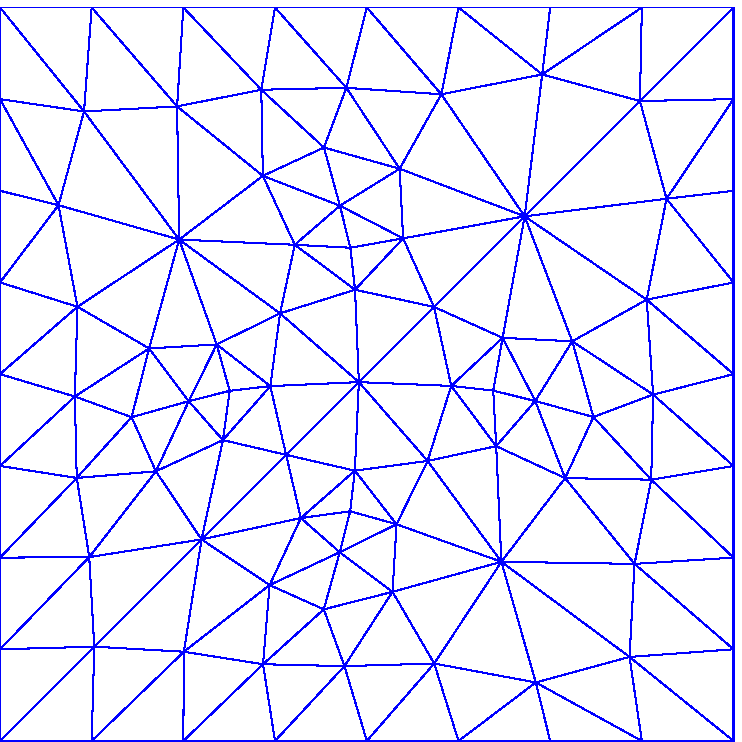
\includegraphics[width=.25\textwidth]{figures/u00.pdf}  \qquad 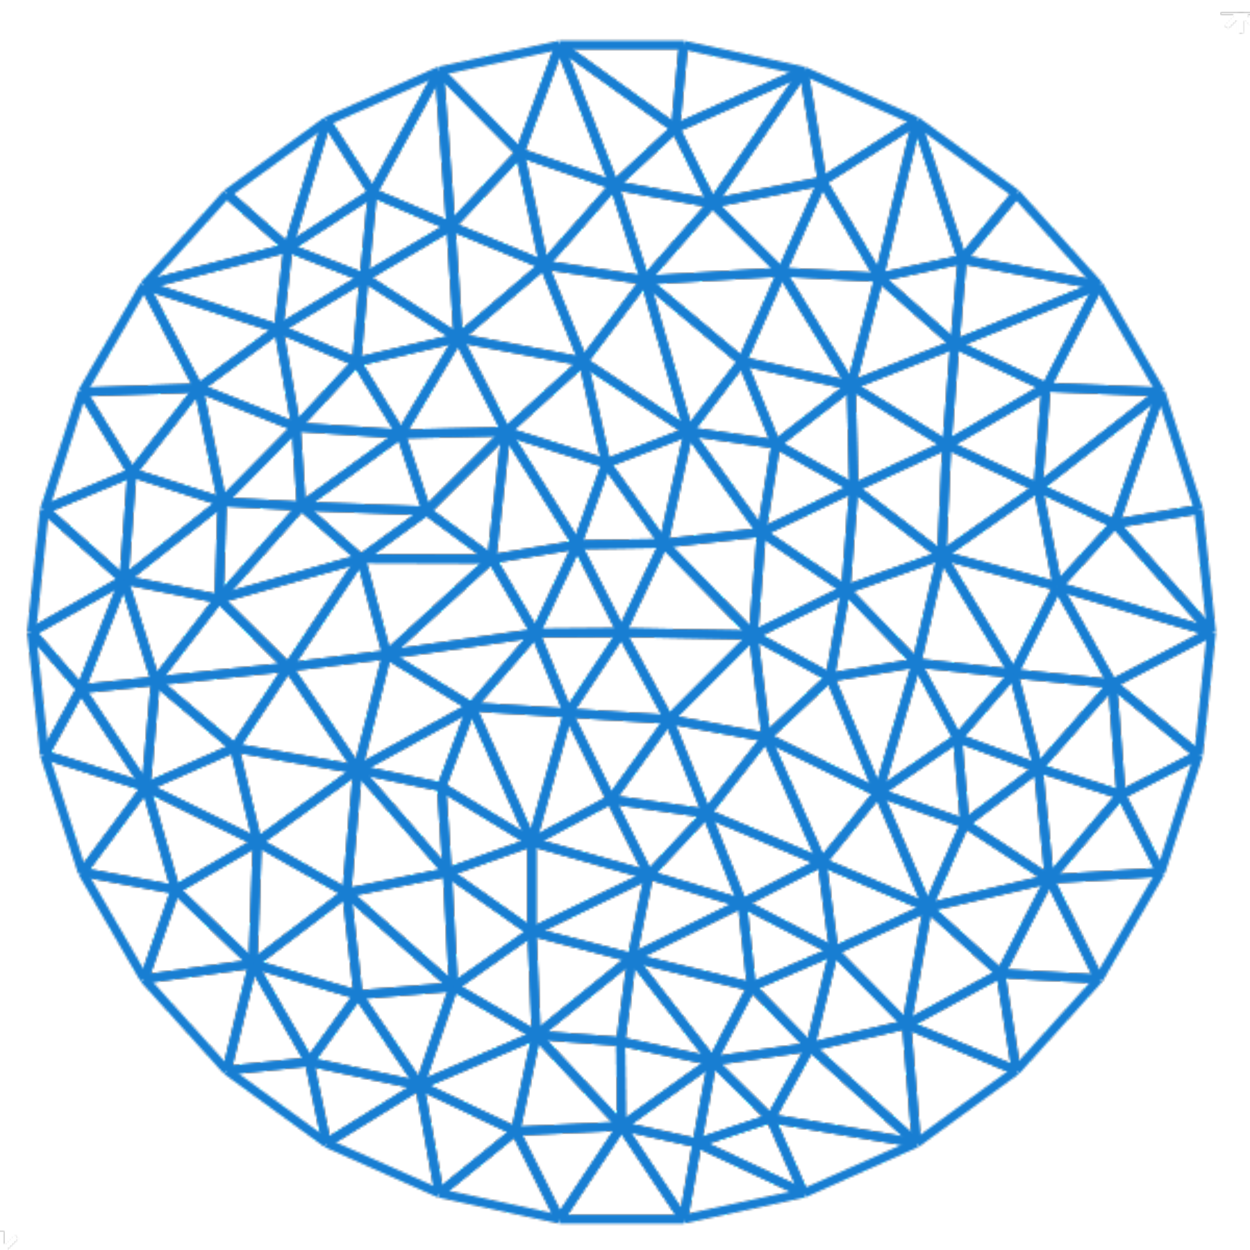
\includegraphics[width=.25\textwidth]{figures/2ddiskpartition.pdf}  
\end{center}
\caption{2D grids}
\label{2duniform}
\end{figure}

Denote 
$$
h_\tau=\mbox{\rm diam} (\tau)\quad  \hbox{(diameter of the smallest sphere containing $\overline{\tau}$)},
$$
and 
$$
 h=\max_{\tau\in\mathcal T_h} h_\tau;\quad
\underline{h}=\min_{\tau\in\mathcal T_h} h_\tau.
$$
A set of triangulations $\mathscr T$ is called {\em shape regular} if
there exists a constant $c_0$ such that
\begin{equation}\label{shape} \max _{\tau \in \mathcal T_h} \frac{h_{\tau}^d}{|\tau|}\leq c_0, \quad \forall \, \mathcal T_h\in
\mathscr T,
\end{equation} 
where $|\tau|$ is the measure of $\tau$ in $\mbb R^d$. This assumption can also be represented as
\begin{equation}\Label{A3.1}
\max_{\tau\in\ct_h}\frac{h_\tau}{\rho_\tau}\le\sigma_1,\quad \forall \, \mathcal T_h\in
\mathscr T,
\end{equation}
where $\rho_\tau$\index{$\rho_\tau$} denotes the radius of the ball
inscribed in $\tau$. In two dimensions, it is equivalent
to the minimal angle of each triange is bounded below uniformly
in the shape regular class. 
%We shall define $h_{\tau} = |\tau|^{1/n}$
%for any $\tau \in \mathcal T_h\in \mathscr T$. By (\ref{shape}),
%$h_{\tau}\eqsim {\rm diam}(\tau)$ represents the size of an element
%$\tau \in \mathcal T_h$ for a shape regular triangulation $\mathcal T_h\in
%\mathscr T$.

In addition to (\ref{shape}), if
\begin{equation}\Label{A3.2}
  \frac{\max _{\tau \in \mathcal T_h}|\tau|}{\min _{\tau \in \mathcal T_h}|\tau|} \leq \rho,\quad \forall \, \mathcal T_h\in \mathscr T,
\end{equation}
$\mathscr T$ is called {\em quasi-uniform}. For quasi-uniform grids,
$h=\max _{\tau \in \mathcal T_h} h_{\tau}$, the mesh size of
$\mathcal T_h$, is used to measure the approximation rate. 
%In the FEM literature, we often write as $\mathcal T_h$.

%The triangulation $\thset$ is said to be quasi-uniform
%\index{triangulation, quasi-uniform} if it satisfies \rf{A3.1} and
%the following
%\begin{eqhttps://gmu.zoom.us/j/97581839555?pwd=ZjlZeFE3Q0JkekdOcGpBZEZxdFJwQT09uation}\Label{A3.2}
%h\le\sigma_3 \underline {h}.
%\end{equation}

The assumption \rf{A3.1} is a local assumption, as is meant by above
definition, for $d=2$ for example, it assures that each triangle will
not degenerate into a segment in the limiting case.  
%A triangulation satisfying this assumption is often called to be {\it shape regular}.

On the other hand, the assumption \rf{A3.2} is a global assumption,
which says that the smallest mesh size is not too small compared with
the largest mesh size of the same triangulation.  By the definition, in
a quasi-uniform triangulation, all the elements are about the same size
asymptotically.

Let $ x_{i}=(x^1_{i}, \cdots, x^d_{i})^t, i=1,\cdots, d+1$ be $d+1$ points in $\mbb R^d$ which do not all lie in one hyper-plane. 
The {\it convex hull} of the $d+1$ points $ x_1, \cdots,  x_{d+1}$ (See Figure \ref{fig:barycentricCoor})
\begin{equation}
\tau :=\{ x=\sum _{i=1}^{d+1}\lambda _i x_i \, | \, 0\leq \lambda_i\leq 1, i=1:d+1, \sum _{i=1}^{d+1}\lambda _i=1 \}
\end{equation}
is defined as a {\em geometric $d$-simplex} generated (or spanned) by
the vertices $ x_1, \cdots,  x_{d+1}$. For example, a triangle
is a $2$-simplex and a tetrahedron is a $3$-simplex. For an integer
$0\leq m \leq d-1$, an $m$-dimensional face of $\tau$ is any
$m$-simplex generated by $m+1$ of the vertices of
$\tau$. Zero-dimenisonal faces are vertices and one-dimensional faces
are called edges of $\tau$. The $(d-1)$-face opposite to the vertex
$ x_i$ will be denoted by $F_i$.
\begin{figure}[hpt]
%\subfigure[1d simplex]{
%\begin{minipage}[t]{0.33\linewidth}
\centering
\includegraphics*[width=2.5cm]{figures/barycentricCoor1D.pdf}
%\end{minipage}}%%
%\subfigure[2d simplex]{
%\begin{minipage}[t]{0.33\linewidth}
%\centering
\includegraphics*[width=3cm]{figures/barycentricCoor2D.pdf}
%\end{minipage}}%%
%\subfigure[3d simplex]
%{\begin{minipage}[t]{0.33\linewidth}
%\centering
\includegraphics*[width=3.1cm]{figures/barycentricCoor3D.pdf}
%\end{minipage}}
\caption{Geometric explanation of barycentric coordinates}
\label{fig:barycentricCoor}
\end{figure}
%\paragraph{Barycentric coordinates}
On the other hand, for any $ x\in \tau$, there exist unique numbers $\lambda _1,\cdots, \lambda _{d+1}$ satisfying $\displaystyle 0\leq \lambda_i\leq 1, i=1:d+1, \sum _{i=1}^{d+1}\lambda _i=1$ such that $\displaystyle x=\sum _{i=1}^{d+1}\lambda _i x_i$, thus we can denote $\lambda _1,\cdots, \lambda _{d+1}$ as $\lambda _1( x),\cdots, \lambda _{d+1}( x)$. In fact,  the numbers $\lambda _1( x),\cdots, \lambda _{d+1}( x)$ are
called {\em barycentric coordinates} of $ x$ with respect to the
$d+1$ points $ x_1, \cdots,  x_{d+1}$. There is a simple
geometric meaning of the barycentric coordinates. Given a $ x\in
\tau$, let $\tau _i( x)$ be the simplex with vertices $ x_i$
replaced by $ x$. Then it can be easily shown that
\begin{equation}\label{eq:lambdasolution}
\lambda _i( x) = |\tau _i( x)|/|\tau|,
\end{equation}
where $|\cdot|$ is the Lebesgure measure in $\mbb R^d$, namely area in
two dimensions and volume in three dimensions. Note that $\lambda
_i( x)$ is affine function of $ x$ and vanishes on the face
$F_i$. We list the four basic properties of barycentric coordinate below:
\begin{enumerate}
\item $0\leq \lambda_i( x)\leq 1$;
\item $\displaystyle\sum_{i=1}^{d+1} \lambda_i( x)=1$;
\item $\lambda_i( x)\in P_1(\tau)$, where $P_1(\tau)$ denotes the space of polynomials of degree $1$
(linear) on $\tau\in \mathcal T_h$;
\item $\lambda_i( x_j)=\delta_{ij}=\begin{cases}
1, \quad &\text{if}  \quad  i=j\\
0, \quad &\text{if} \quad i\neq j
\end{cases}.$
\end{enumerate}

\subsection{Continuous linear finite element spaces}\label{linearFE}
A conforming linear finite element function in a domain $\Omega\subset
\mathbb R^d$ is a continuous function that is piecewise linear
function with respect to a grid or mesh consisting of a union of simplices.

Given a shape regular triangulation $\mathcal T_h$ of $\Omega$, we define the 
continuous linear finite element space as 
\begin{equation}\label{LinFE}
V_h:=\{v\,|\, v\in C(\overline \Omega), \,\hbox{ and }\, v|_{\tau}\in
P_1(\tau), \forall \tau \in \mathcal T_h\},
\end{equation}
where $P_1(\tau)$ denotes the space of polynomials of degree $1$
(linear) on $\tau\in \mathcal T_h$. Whenever we need to deal with boundary
conditions, we further define $V_{h,0}=V_h\cap H_0^1(\Omega)$.

We note here that the global continuity is also necessary in the
definition of $V_h$ in the sense that if $u$ has a square interable
gradient, that is $u\in H^1(\Omega)$, and $u$ is piecewise smooth,
then $u$ is continuous. 

We always use $n_h$ to denote the dimension of finite element
spaces. For $V_h$, $n_h$ is the number of vertices of the
triangulation $\mathcal T_h$ and for $V_{h,0}$, $n_h$ is the number of
interior vertices. 

\paragraph{Nodal basis functions and dual basis}
For linear finite element spaces, we have the so
called \emph{a standard nodal basis functions} $\{\varphi
_i,i=1,\cdots n_h\}$ such that $\varphi_i$ is piecewise linear (with
respect to the triangulation) and $\varphi_i(x_j)=\delta_{i,j}$.  Note
that $\varphi _i|_\tau$ is the corresponding barycentrical coordinates
of $x_i$. See Figure \ref{fig:nodalbasis} for an illustration in 2D.
\begin{figure}[hpt]
%\subfigure[1d basis function]{
%\begin{minipage}[t]{0.49\linewidth}
\centering
\includegraphics*[height=4.5cm,width=7cm]{6DL/figures/Dualbasis}
%\end{minipage}}
\caption{Dual basis functions of $V_h$ in 1D for $n_h=5$.}
\label{fig:dualbasis}
\end{figure}
Let $(\varphi_i^*)_{i=1}^{n_h}$ be the dual basis of $(\varphi_i)_{i=1}^{n_h}$, namely
\begin{equation}
  \label{eq:1}
(\varphi_i^*, \varphi_j) =\delta_{i, j}, \quad i, j=1,\ldots, n_h.    
\end{equation}
We notice that all the nodal basis functions $\{\varphi_i\}$ are locally
supported, but their dual basis functions $\{\varphi_i^*\}$ are in general
not locally supported (see Figure \ref{fig:dualbasis}).  The nodal basis functions $\{\varphi_i\}$ are
easily constructed in terms of barycentric coordinate functions.  The
dual basis $\{\varphi_i^*\}$ are only interesting for theoretical
consideration and it is not necessary to know the actual constructions
of these functions.

%
\begin{figure}[hpt]
%\subfigure[1d basis function]{
%\begin{minipage}[t]{0.49\linewidth}
\centering
\includegraphics*[height=4.5cm,width=7cm]{figures/basisfunction}
%\end{minipage}}%%
%\subfigure[2d basis function]{
%\begin{minipage}[t]{0.49\linewidth}
%\centering
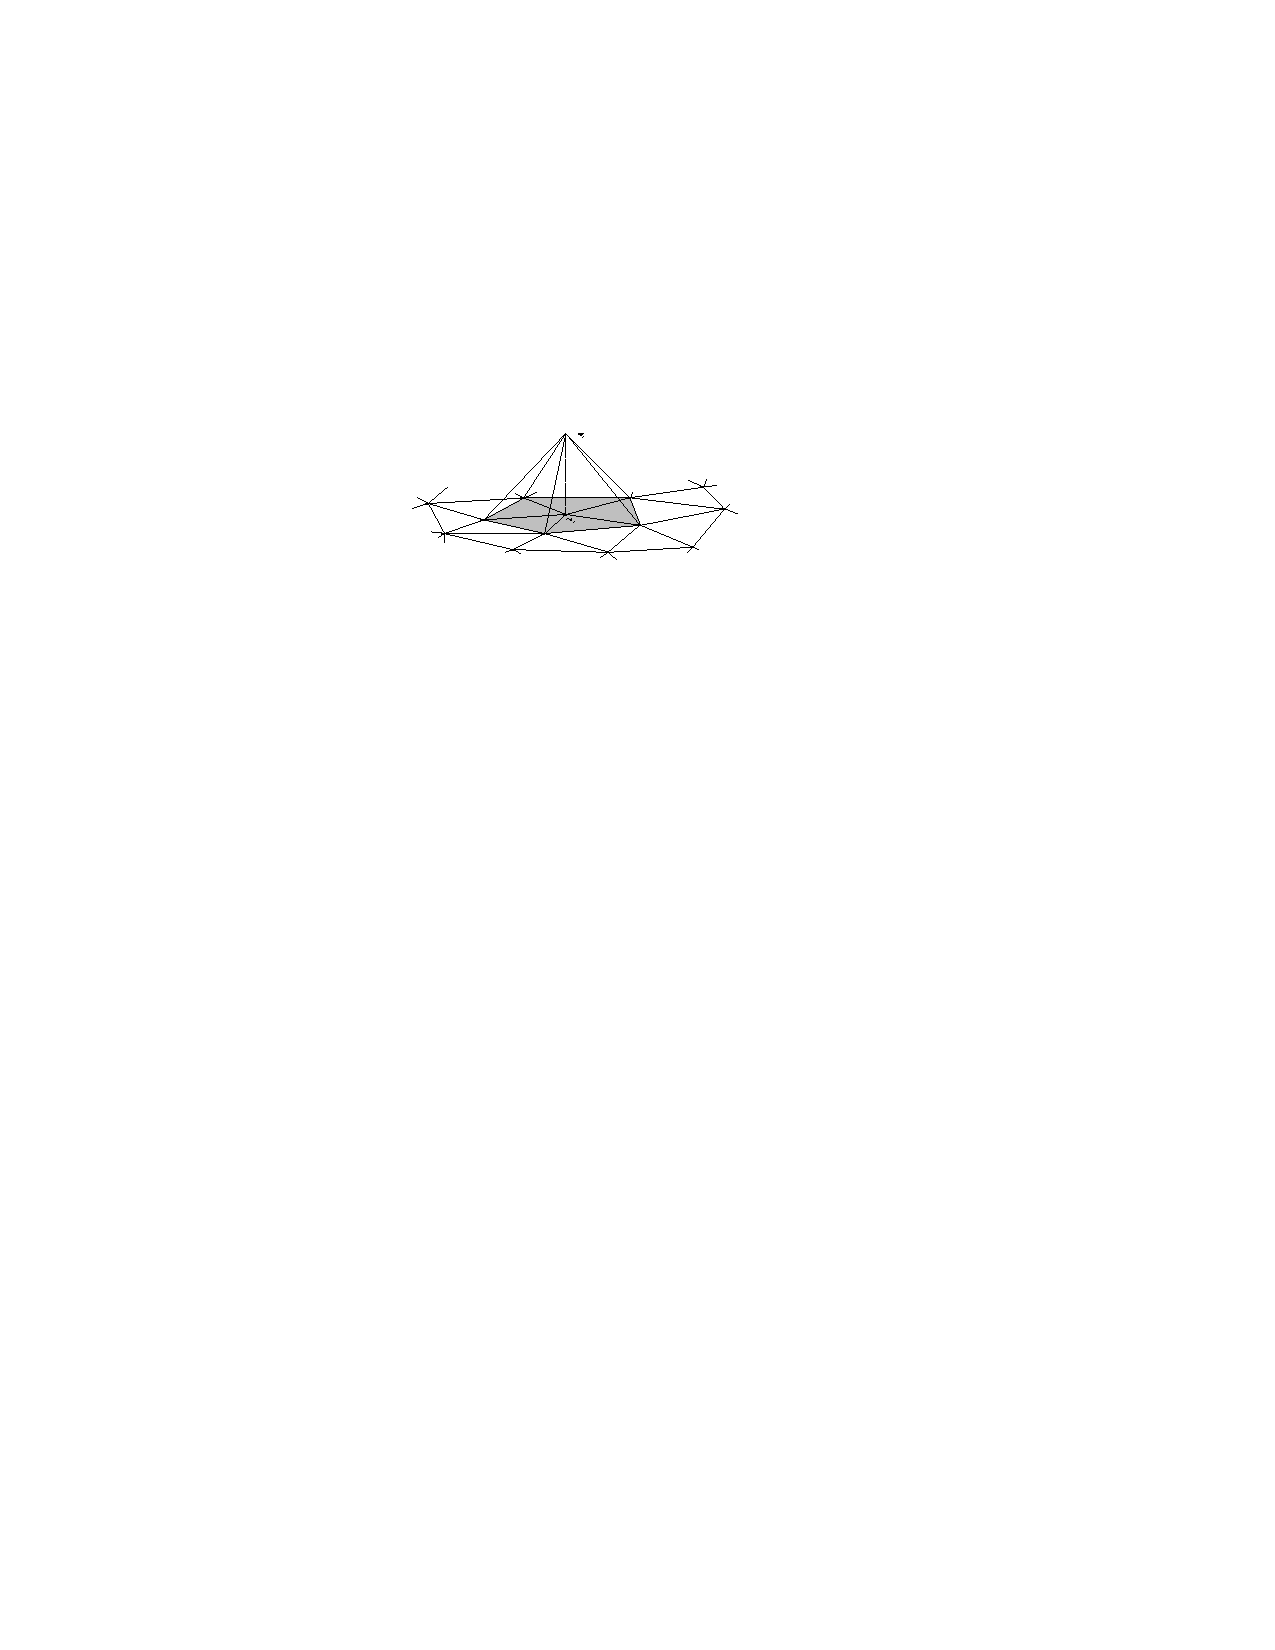
\includegraphics[height=5cm,width=7cm]{figures/nodalbasis.pdf}
%\end{minipage}}
\caption{Nodal basis functions in 1d and 2d}
\label{fig:nodalbasis}
\end{figure}
Since $\{\varphi_i,i=1,\cdots n_h\}$ is a basis of $V_h$, therefore for any $v_h\in V_h$, we have the representation
$$
v_h(x)=\sum_{i=1}^{n_h}v_h(x_i)\varphi_i(x). 
$$

Let us see how our construction of continuous linear finite space and the nodal basis looks like  in one spatial dimension. 
Associated with the mesh
$$
\mathcal T_h=\{0=x_0<x_1<\ldots<x_{n_h}<x_{n_h+1}=1\},
$$
by the definition given in \eqref{LinFE} and the definition  $V_{h,0}=V_{h}\cap H_0^1(\Omega)$, we have
\[
\begin{array}{ll}
V_{h,0}=\{v:~\mbox{$v$ is continuous and piecewise linear}~ \mbox{w.~r.~t. $\mathcal T_h$, } v(0)=v(1)=0\}.
\end{array}
\]
A plot of a typical element of $V_{h,0}$ is shown in Fig.~\ref{fig:1dtypical}.

It is easily calculated (as we already mentioned), that the dimension
of $V_{h,0}$ is equal to the number of internal vertices, and the nodal
basis functions spanning $V_{h,0}$ (for $i=1,2,\cdots,n_h$) are (see also
Fig.~\ref{fig:nodalbasis}):
\begin{equation}\label{1dbasis:function}
\varphi_i(x)=\left\{\begin{array}{cl}
\displaystyle \frac{x-x_{i-1}}{h}, & x\in[x_{i-1},x_i];\\
\displaystyle \frac{x_{i+1}-x}{h}, & x\in[x_{i},x_{i+1}];\\
0 &\mbox{elsewhere}.
\end{array}\right.
\end{equation}

\begin{figure}[hpt]
\centering
\includegraphics*[width=2in]{figures/femfunction1.pdf}
\caption{Plot of a typical element from $V_{h,0}$.} 
\label{fig:1dtypical}
\end{figure}



%%%%%%%%%%%%%%%%%%%%END from grid.tex%%%%%%%%%%%%%%%%%%%%%%%%%%%%%%%

%%%%%%%%%%%%%%%%%%%%END from grid.tex%%%%%%%%%%%%%%%%%%%%%%%%%%%%%%%

%%%%%%%%%%%%%%%%%%%%END from grid.tex%%%%%%%%%%%%%%%%%%%%%%%%%%%%%%%

\section{Motivation: from finite element to neural network}\label{FE2NN}
In this section, we will introduce the so-called shallow neural network 
(deep neural network with one hidden layer) from the viewpoint of finite element method.

Let us recall the linear finite element functions on the unit interval $\bar{\Omega}=[0,1]$ in Section \ref{linearFE}. 
Consider a set of equidistant girds $\mathcal T_\ell$ of level $\ell$ and mesh length $h_\ell = 2^{-\ell}$. The grid points $x_{\ell,i}$ are given by
\begin{equation}
x_{\ell,i}:=ih_\ell,\quad 0\le i\le 2^\ell.
\end{equation} 
For $\ell=1$, we denote the special hat function by $\varphi(x)$ and any nodal basis function in \eqref{1dbasis:function} on grid $\mathcal T_\ell$ by $\varphi_{\ell,i} $ as below
\begin{equation}\label{def_g}
\varphi(x) = 
\begin{cases}
2x \quad &x\in [0,\frac{1}{2}] \\
2(1-x) \quad &x\in [\frac{1}{2}, 1] \\
0, \quad &\text{others} 
\end{cases},\qquad
\varphi_{\ell,i} = \varphi(\frac{x - x_{\ell,i-1}}{2h_\ell}) = \varphi(w_\ell x + b_{\ell,i}).
\end{equation} 
That is to say, any $\varphi_{\ell,i}(x)$ can be obtained from $\varphi(x)$ by scaling 
(dilation) and translation with 
\begin{equation}\label{key}
w_\ell = 2^{\ell-1}, \quad b_{\ell,i} = \frac{-(i-1)}{2},
\end{equation}
in $\varphi_{\ell,i} = \varphi(w_\ell x + b_{\ell,i})$. 
\begin{figure}[H]
\centering
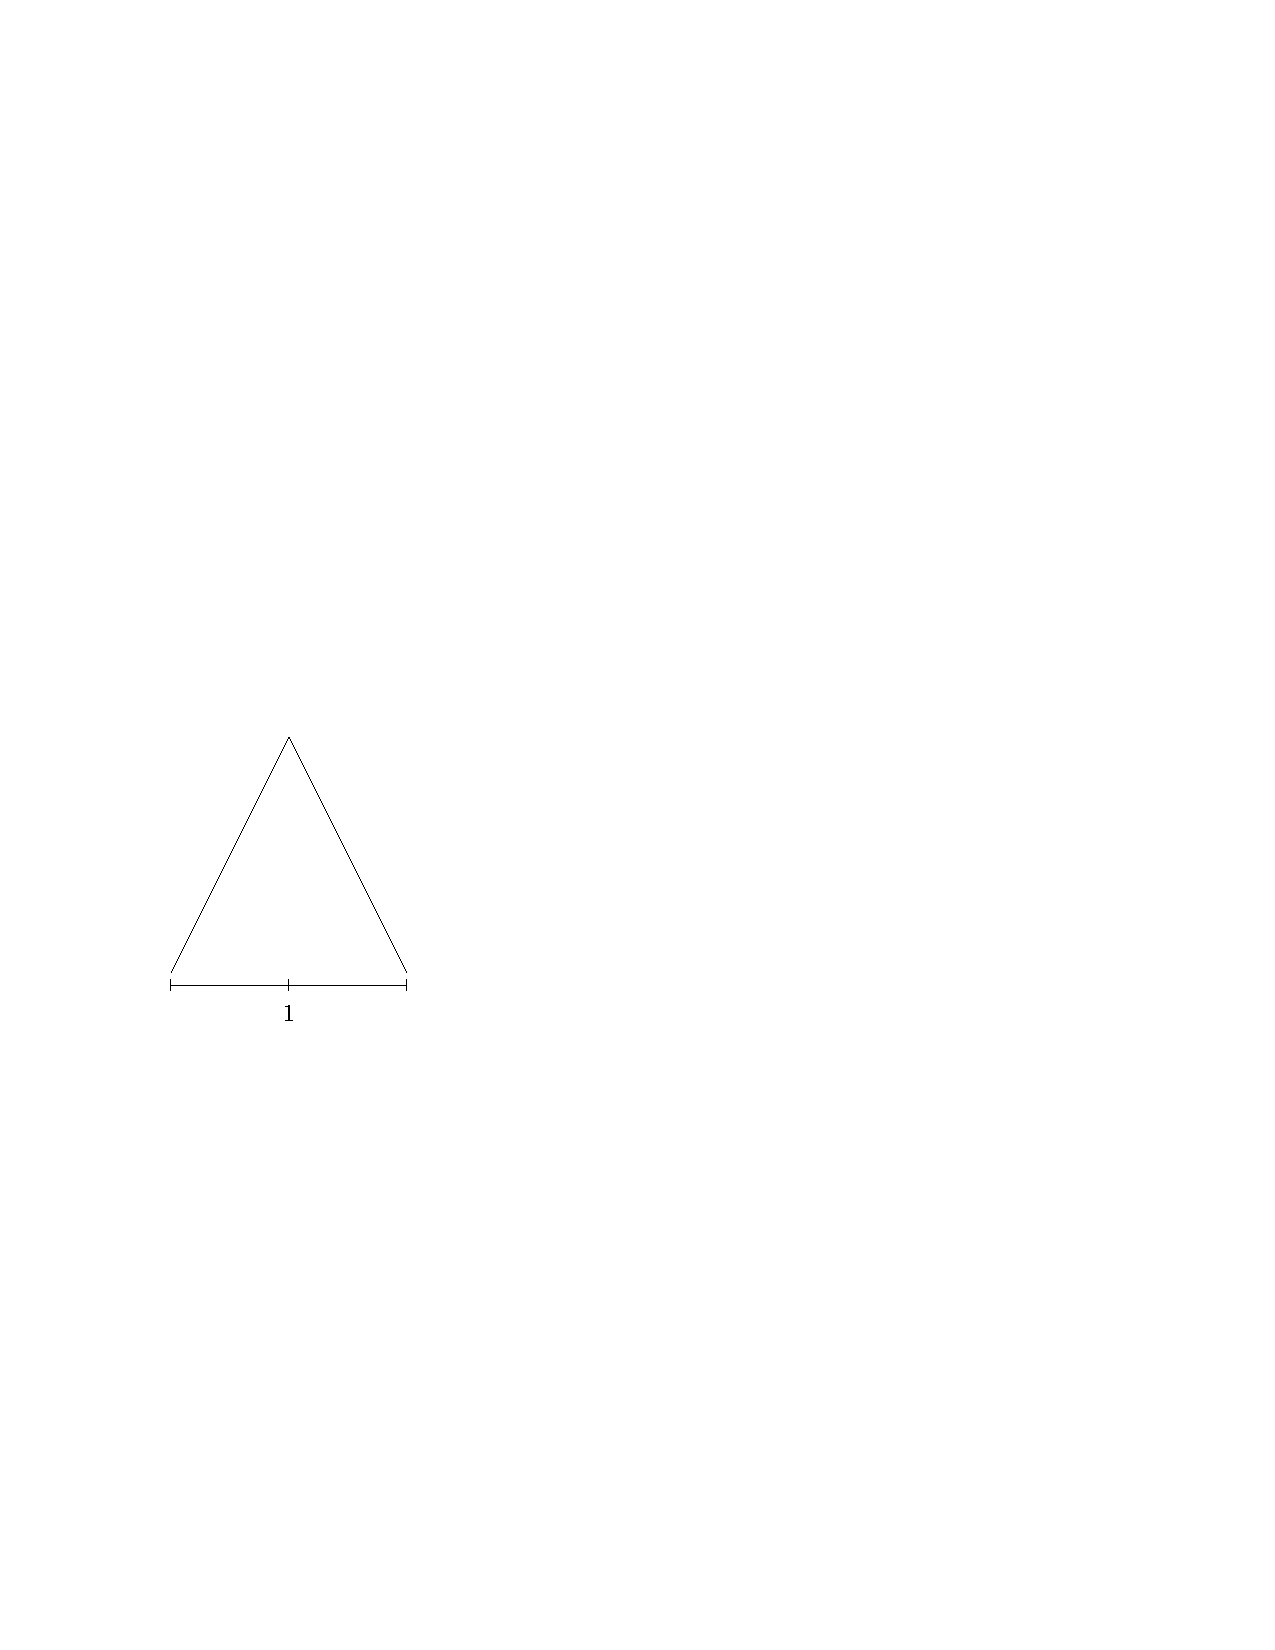
\includegraphics[width=4cm]{1dbasis1.pdf}\qquad
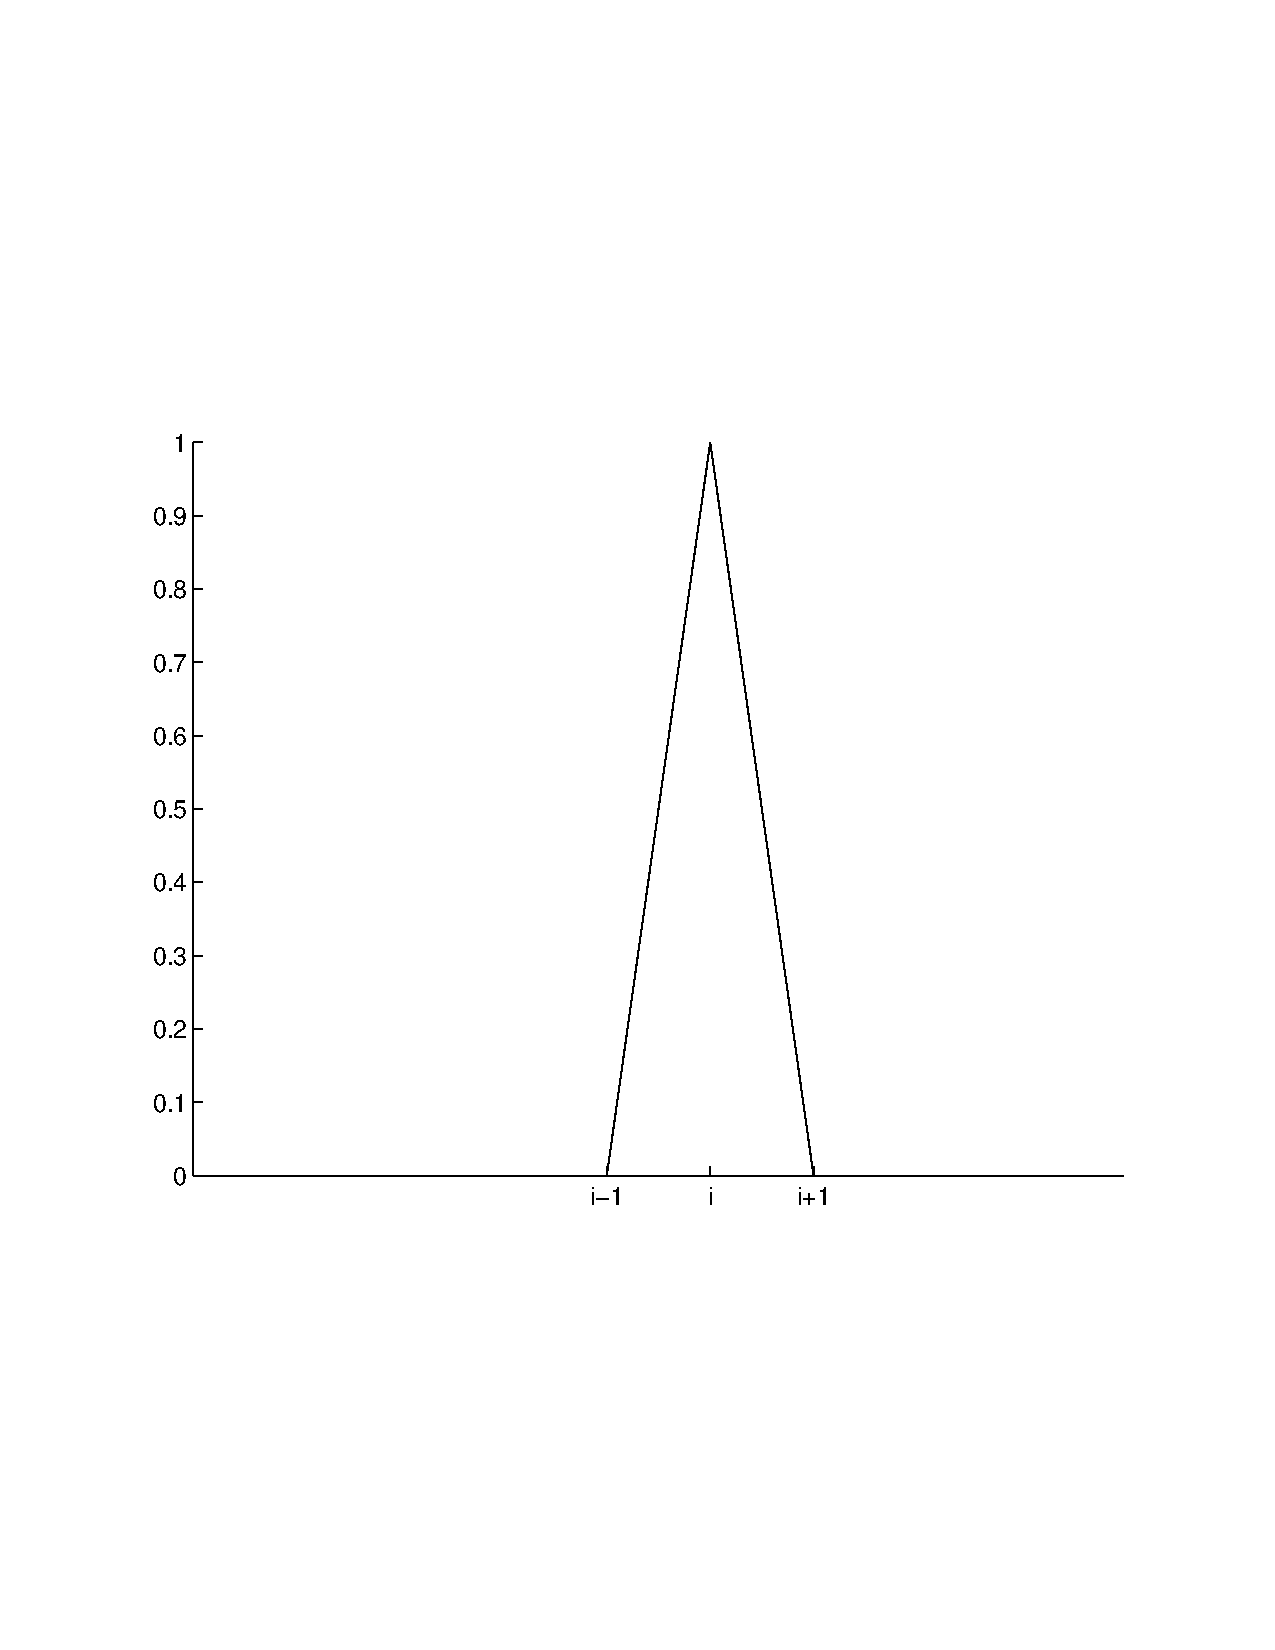
\includegraphics[width=5cm]{basisfunction.pdf}
\caption{Diagram of $\varphi(x)$ (left) and $\varphi_{\ell,i}(x)$ (right).}
\end{figure} 


Let us recall the finite element interpolation in Section \ref{linearFE} as
\begin{equation}\label{key}
u(x) \approx u_\ell(x) := \sum_{ 0\le i \le 2^\ell} u(x_{\ell,i}) \varphi_{\ell,i}(x),
\end{equation}
for any smooth function $u(x)$ on $(0,1)$. The above interpolation will converge as $\ell \to \infty$, which shows that
\begin{equation}\label{key}
{\rm span} \left\{  \varphi(w_\ell x + b_{\ell,i}) \right\} \quad \text{is dense in} \quad H^1(0,1).
\end{equation}
Thus, we may have the next concise relation:
\begin{equation}\label{key}
\begin{split}
\text{FE space} =  &{\rm span} \left\{  \varphi(w_\ell x + b_{\ell,i}) ~|~ 0\le i \le 2^\ell, \ell = 1, 2, \cdots \right\} 
\\
\subset  &{\rm span} \left\{  \varphi(w x + b) ~|~  w, b \in \mathbb{R} \right\}.
\end{split}
\end{equation}
In other words, the finite element space can be understood as the linear combination of $\varphi(w x + b)$ with certain special choice of $w$ and $b$. 

Here, we need to point out that this ${\rm span} \left\{  \varphi(w x + b) ~|~  w, b \in \mathbb{R} \right\}$ is exact the deep neural networks with one hidden layer (shallow neural networks) with activation function $\varphi(x)$. More precisely, 
\begin{equation}\label{key}
f \in {\rm span} \left\{  \varphi(w x + b) ~|~  w, b \in \mathbb{R} \right\},
\end{equation}
means there exist positive integer $N$ and $w_j, b_j \in \mathbb{R}$ such that 
\begin{equation}\label{key}
f = \sum_{j=1}^N a_j \varphi(w_j x + b_j),
\end{equation}
which is also called one hidden neural network function with $N$ neurons.

\begin{remark}
	\begin{enumerate}
		\item By making $w_\ell$ and $b_{\ell,i}$ in \eqref{def_g} arbitrary, we get a much larger class of 
		function which is exact a special neural network with activation function $\varphi(x)$.
		\item Generalizations: 
		\begin{enumerate}
			\item activation function $\varphi$ can be different, such as ${\rm ReLU}(x) = \max\{0,x\}$.
			\item There is a natural extension for high dimension $d$ as
			\begin{equation}\label{key}
			\left\{  \varphi(w\cdot x + b) \right \},
			\end{equation}
			where $w\in \mathbb{R}^d$, $b\in \mathbb{R}$ and $\displaystyle w\cdot x = \sum_{i=1}^d w_i x_i$.
			This is called ``deep'' neural network with one hidden layer.
		\end{enumerate}
	\end{enumerate}
\end{remark}


%\input{3FEM/2dFEM}

\section{Why we need deep neural networks via composition}\label{whydeep}
\subsection{FEM ans ${\rm DNN}_1$ in 1D}
Thanks to following connection between $\varphi(x)$ in \eqref{def_g} and ${\rm ReLU}(x) = \max(0,x )=x_+$
\begin{equation}\label{key}
\varphi(x) = 2{\rm ReLU}(x) - 4{\rm ReLu}({x-\frac{1}{2}}) + 2{\rm ReLU}(x-1),
\end{equation}
it suffices to show that each basis
function $\varphi_{\ell,i}$ can be represented by a ReLU DNN. 
We first note that  the basis
function $\varphi_{\ell,i}$ has the support in $[x_{\ell,i-1},
x_{\ell,i+1} ]$ can be easily written as
\begin{equation}
\label{1d-basisu}
\varphi_{\ell,i}(x) = \frac{1}{h_{\ell}}{\rm ReLU}(x-x_{\ell,i-1}) -\frac{2}{h_{\ell}}{\rm ReLU}(x-x_{\ell,i}) +\frac{1}{h_\ell}{\rm ReLU}(x-x_{\ell,i+1}).
\end{equation}
More generally, consider a general  grid with vertex $\{x_i\}$, which is not necessarily uniform. The basis function $\varphi_i$ of the linear element with support $[x_{i-1},
x_{i+1} ]$ can be easily written as
\begin{equation}
\label{1d-basis}
\varphi_i(x) = \frac{1}{h_{i-1}}{\rm ReLU}(x-x_{i-1}) -(\frac{1}{h_{i-1}}+\frac{1}{h_i}){\rm ReLU}(x-x_i) +\frac{1}{h_i}{\rm ReLU}(x-x_{i+1}),
\end{equation}
where $h_i = x_{i+1} - x_i$.

Thus is to say, we have the next theorem.
\begin{theorem}\label{thm:1dLFEMDNN}
	For $d=1$, and  $\Omega\subset \mathbb R^d$ is 
	a bounded interval, then ${\rm DNN}_1$ can be used to cover all linear finite element 
	function in on $\Omega$.
\end{theorem}
\subsection{Linear finite element cannot be recovered by ${\rm DNN}_1$ for $d\ge2$}
In view of  Theorem~\ref{thm:1dLFEMDNN} and the fact that ${\rm{DNN}_J}
\subseteq {\rm{DNN}_{J+1}} $, it is natural to ask that how many
layers are needed at least to recover all linear finite element
functions in $\mathbb{R}^d$ for $d\ge2$.  In this section, we will show that 
\begin{equation}\label{key}
J_d \ge 2, \quad \text{if} \quad d\ge 2,
\end{equation}
where $J_d$ is the minimal $J$ such that all linear finite element
functions in $\mathbb R^d$ can be recovered by ${\rm DNN}_J$.

In particular, we will show the following theorem~\cite{he2020relu}.
\begin{theorem}\label{lowerbound}
	If $\Omega\subset \mathbb R^d$ is either 
	a bounded domain or $\Omega=\mathbb{R}^d$,  
	${\rm DNN}_1$ can not be used to recover all linear finite element
	functions on $\Omega$. 
\end{theorem}
\begin{proof}
	We prove it by contradiction. Let us assume that for any continuous
	piecewise linear function $f: \Omega \to \mathbb{R} $, we can find
	finite $N \in \mathbb{N}$, $w_i \in \mathbb{R}^{1,d}$ as row vector
	and $\alpha_i, b_i, \beta \in \mathbb{R}$ such that
	$$
	f =  \sum_{i=1}^N \alpha_i {\rm ReLU}(w_i\cdot  x +b_i) + \beta,
	$$
	with $f_i = \alpha_i {\rm ReLU}(w_i\cdot  x +b_i)$, $\alpha_i \neq 0$ and $w_i
	\neq 0$.  Consider the finite element functions, if this one hidden
	layer ReLU DNN can recover any basis function of FEM, then it can
	recover the finite element space.  Thus let us assume $f$ is a locally
	supported basis function for FEM.
	Furthermore, if $\Omega$ is a bounded domain, we assume that 
	\begin{equation}\label{distcondi}
	d({\rm supp}(f), \partial \Omega) > 0,
	\end{equation}with 
	$$
	d(A, B) = \inf_{x\in A, y\in B} \|x-y\|,
	$$ 
	as the distance of two closed sets. 
	
	A more important observation is that $\nabla f: \Omega \to
	\mathbb{R}^d$ is a piecewise constant vector function. The key
	point is to consider the discontinuous points for 
	$$g := \nabla
	f = \sum_{i=1}^N \nabla f_i.$$
	For more general case, we can define the set of discontinuous points of a function by
	$$
	D_{g} := \{x \in \Omega~|~ x ~ \text{is a discontinuous point of} ~ g\}.
	$$
	Because of the property that 
	\begin{equation}\label{eq:disfun}
	D_{f+g} \supseteq D_{f} \cup D_{g} \backslash (D_{f} \cap D_{g}),
	\end{equation}
	we have
	\begin{equation}\label{eq:dis_fn}
	D_{\sum_{i=1}^N g_i} \supseteq \bigcup_{i=1}^N D_{g_i} \backslash \bigcup_{i\neq j}\left( D_{g_i}\cap D_{g_j} \right).
	\end{equation}
	Note that
	\begin{equation}\label{eq:def_gi}
	g_i = \nabla f_i(x) =  \nabla \left( \alpha_i {\rm ReLU}(w_i\cdot   x +b_i)  \right) =\left(\alpha_iH(w_i \cdot  x +b_i)\right)w_i \in \mathbb{R}^d,
	\end{equation}
	for $i=1:N$ with $H$ be the Heaviside function defined as: 
	$$
	H(x) = \begin{cases}
	0 &\text{if} ~ x \le 0, \\
	1 &\text{if} ~ x > 0.
	\end{cases}
	$$ 
	This means that 
	\begin{equation}\label{eq: D_gi}
	D_{g_i} = \{ x ~|~ w_i\cdot   x + b_i = 0\}
	\end{equation}
	is a $d-1$ dimensional affine space in $\mathbb{R}^d$.  
	
	
	Without loss of generality, we can assume that 
	\begin{equation}\label{eq:assumD_gi}
	D_{g_i} \neq D_{g_j}.
	\end{equation}
	When the other case occurs, i.e. $D_{g_{\ell_1}} = D_{g_{\ell_2}} = \cdots= D_{g_{\ell_k}}$, by the definition of $g_i$ in \eqref{eq:def_gi} and $D_{g_i}$ in \eqref{eq: D_gi} , 
	this happens if and only if there is a row vector $(w, b)$ such that
	\begin{equation}\label{eq:Dfcondition}
	c_{\ell_i}\begin{pmatrix}
	w &
	b
	\end{pmatrix} =  
	\begin{pmatrix}
	w_{\ell_i} &
	b_{\ell_i}
	\end{pmatrix},
	\end{equation}
	with some $c_{\ell_i} \neq 0$ for $i = 1:k$.  We combine those $g_{\ell_i}$ as
	\begin{equation*}
	\begin{aligned}\label{mergeH}
	%	\begin{split}
	\tilde g_{\ell} &= \sum_{i=1}^k g_{\ell_i} = \sum_{i=1}^k \alpha_{\ell_i} H(w_{\ell_i} \cdot  x + b_{\ell_i}) w_{\ell_i}, \\
	&= \sum_{i=1}^k \left( c_{\ell_i}\alpha_{\ell_i} H\left(c_{\ell_i}(w\cdot   x + b)\right) \right) w, \\
	&=\begin{cases}
	\displaystyle \left(\sum_{i=1}^k  c_{\ell_i}\alpha_{\ell_i} H(c_{\ell_i}) \right) w  \quad &\text{if} \quad w x + b > 0,\\
	\displaystyle \left(\sum_{i=1}^k  c_{\ell_i}\alpha_{\ell_i} H(-c_{\ell_i}) \right) w  \quad &\text{if} \quad w x + b \le 0.\\
	\end{cases}
	%	\end{split}
	\end{aligned}
	\end{equation*}	
	Thus, if 
	$$
	\left(\sum_{i=1}^k  c_{\ell_i}\alpha_{\ell_i} H(c_{\ell_i}) \right)  = \left(\sum_{i=1}^k  c_{\ell_i}\alpha_{\ell_i} H(-c_{\ell_i}) \right),
	$$
	$\tilde g_\ell$ is a constant vector function, that is to say $D_{\sum_{i=1}^k g_{\ell_i}} = D_{\tilde g_\ell} = \emptyset$. 
	Otherwise, $\tilde g_\ell$ is a piecewise constant vector function with the property that 
	$$
	D_{\sum_{i=1}^k g_{\ell_i}} = D_{\tilde g_\ell} = D_{g_{\ell_i}} = \{ x ~|~ w\cdot  x + b = 0\}.
	$$
	This means that we can use condition \eqref{eq:Dfcondition} as an equivalence relation and split $\{g_i\}_{i=1}^N$ into some groups, and we can combine those $g_{\ell_i}$ in each group as what we do above. After that, we have
	$$
	\sum_{i=1}^N g_i = \sum_{\ell=1}^{\tilde N} \tilde g_{\ell},
	$$
	with $D_{\tilde g_s} \neq D_{\tilde g_t}$.
	Finally, we can have that $D_{\tilde g_s} \cap D_{\tilde g_t}$ is an empty set or a $d-2$ dimensional affine space in $\mathbb{R}^d$.
	Since
	$\tilde N \le N$ is a finite number, 
	$$
	D := \bigcup_{i=1}^N D_{\tilde g_\ell} \backslash \bigcup_{s\neq t}\left( D_{\tilde g_s}\cap D_{\tilde g_t} \right)
	$$
	is an unbounded set. 
	\begin{itemize}
		\item If $\Omega = \mathbb{R}^d$,
		$$
		{\rm supp(f)} \supseteq D_{g} = D_{\sum_{i=1}^N g_i} = D_{ \sum_{\ell=1}^{\tilde N} \tilde g_{\ell}} \supseteq D,
		$$ is contradictory to the assumption that $f$ is locally supported.
		\item If $\Omega$ is a bounded domain, 
		$$
		d(D, \partial \Omega) = 
		\begin{cases}
		s > 0 \quad &\text{if}\quad  D_{\tilde g_i} \cap \Omega = \emptyset, \forall i\\
		0 \quad &\text{otherwise}.
		\end{cases}
		$$
		Note again that all $D_{\tilde g_i}$'s are $d-1$ dimensional affine spaces, while $D_{\tilde g_i} \cap D_{\tilde g_j}$ is either an empty set or a d-2 dimensional affine space. 
		If $d(D, \partial \Omega) > 0$, this implies that $\nabla f$ is continuous in $\Omega$, which contradicts the  assumption that $f$ is a basis function in FEM.
		If $d(D, \partial \Omega) = 0$, this contradicts the previous assumption in \eqref{distcondi}.
	\end{itemize}
	Hence ${\rm DNN}_1$ cannot recover any piecewise linear function in $\Omega$ for $d \ge 2$.
\end{proof}

Following the proof above, we have the following theorem~\cite{he2020relu}.
\begin{theorem}\label{linearindep}
	$\{{\rm ReLU}(w_i\cdot x+b_i)\}_{i=1}^m$ are linearly independent if $(w_i,
	b_i)$ and $(w_j, b_j)$ are linearly independent in
	$\mathbb{R}^{1\times (d+1)} $ for any $i \neq j$.
\end{theorem}






\section{Basic Artificial Neural Network}
Artificial neural networks (ANNs) are biologically inspired computer programs designed to simulate the way in which the human brain processes information.
%This model is just a model for a class of parameterized function with some special function structure which can be presented simply using some simple network graph. This method is began from the approximation of neural network in human.
\subsection{basic element: Nonlinear active function with affine map}
Mc Culloch-Pitts Neuron, also known as M-P Neuron, is the earliest neural network that was discovered in 1943. In this model, the neurons are connected by connection weights, and the activation function is used in binary. The threshold is used to determine whether the neuron will fire or not.

M-P element(approximation of one neuron): this is a very simple example for interpolating a function $f: \mathbb{R}^m \to \mathbb{R}$, with the next definition:
\begin{equation}\label{eq:M-P}
f_{M-P}(x) = \sigma( w \cdot x + b)
\end{equation}
with $w  \in \mathbb{R}^{m} $ and $\sigma$ is called active function which can be chosen like:
\begin{equation}
\sigma (x) = \frac{1}{1 + e^{-x}},
\end{equation}
or
\begin{equation}
\sigma(x) = tanh(x) = \frac{e^x - e^{-x}}{e^x + e^{-x}}.
\end{equation}
Basically, both these two functions are smooth and have two horizontal asymptotic lines, which can be seen as a smoothing approximation for
\begin{equation}
H(x) =
\begin{cases}
1  &\text{if}  ~x < 0, \\
0 &\text{if}~ x \le 0.
\end{cases}
\end{equation}
But now, the most commonly used activation function is the so-called ``Rectified Linear Unit'' (ReLU), which is defined by
\begin{equation}
{\rm ReLU}(x) = \max\{0,x\}.
\end{equation}
%We will talk about some basic stuff about variant of activation function in the next chapter and 
It is also very important in the approximation theory for such as one hidden layer ANN networks.
This is often shown as the next picture:
\begin{figure}[!ht]
	\center{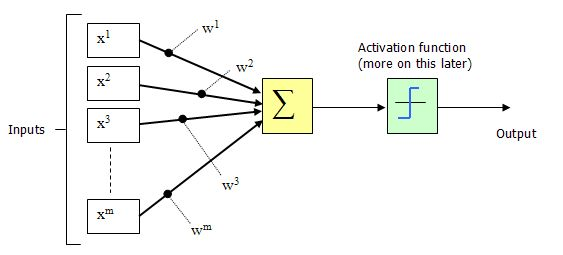
\includegraphics[width=10cm] {M-P.jpeg}}
	\caption{M-P neuron.}
\end{figure}

\subsection{neural network}
Now we want to use this simple basic element to construct some more complex model(from one neuron to neural network). A bionic but simple construction is to increase the basic element in both horizontal and vertical direction, which means the network would be like the one in Fig~\ref{fig:ANN}.
\begin{figure}[!ht]
	\center{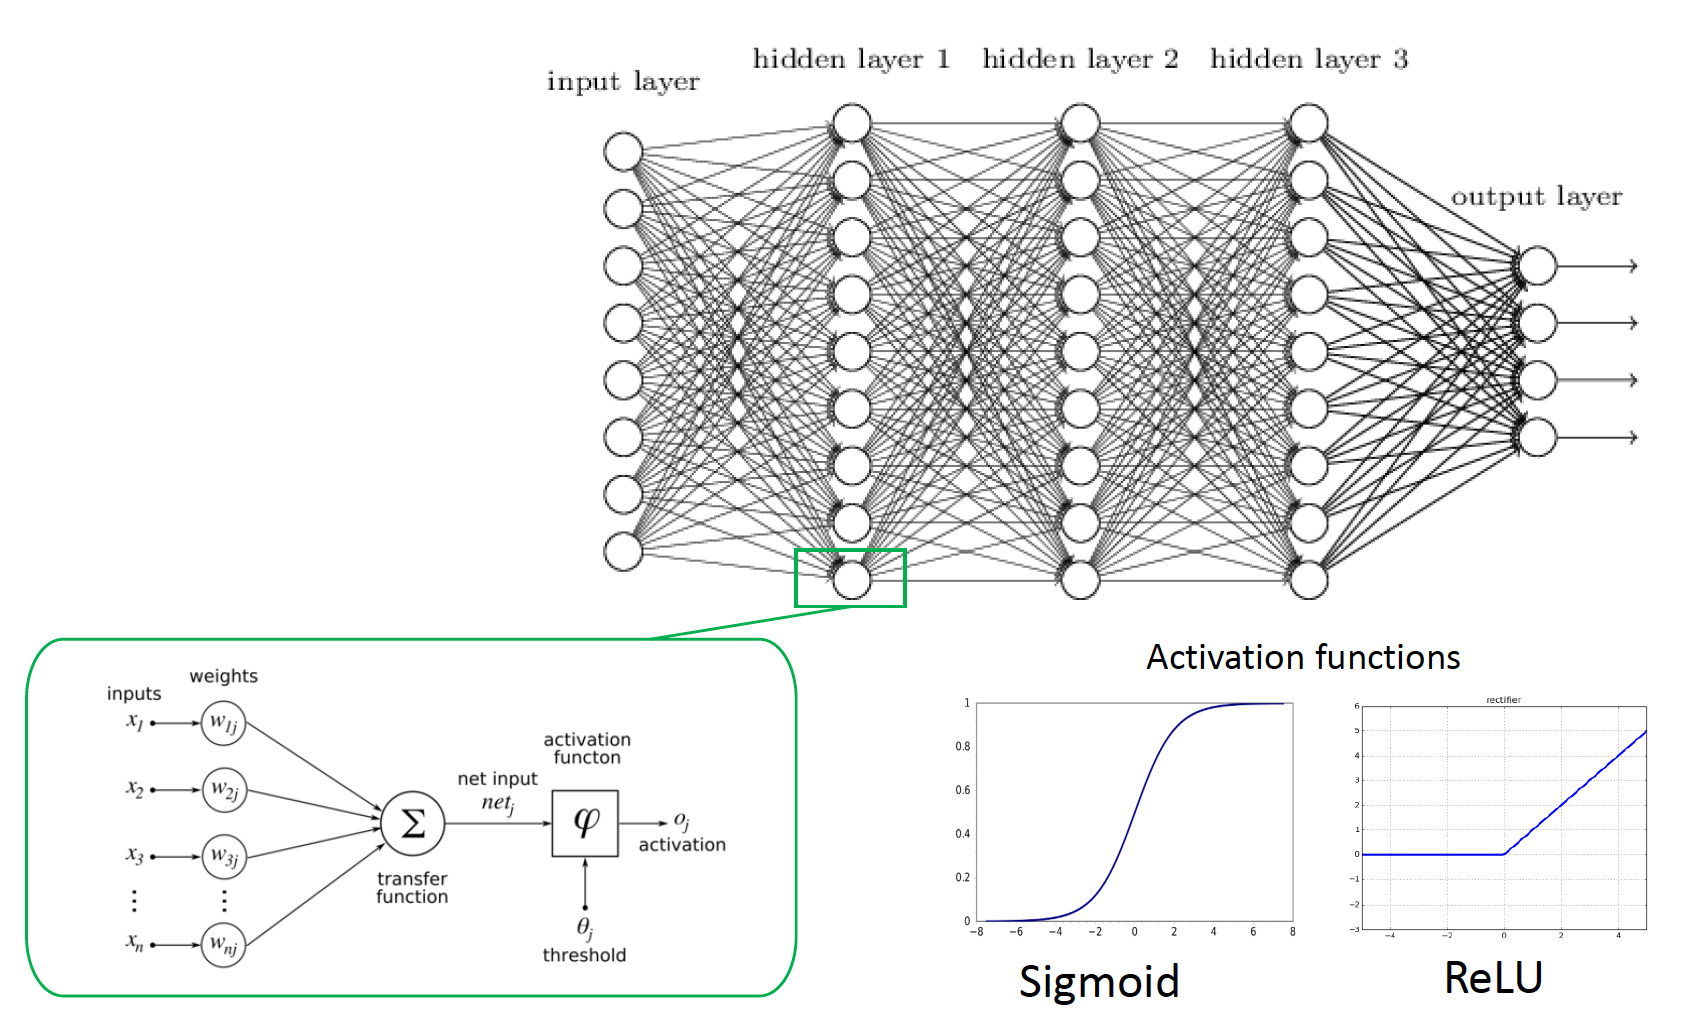
\includegraphics[width=12cm,height=6cm] {ANN.png}}
	\caption{ANN}
	\label{fig:ANN}
\end{figure}

This is called fully connected feedforward neural network. Now we want to give a more compressive expression, we collect all the output in $k$-th level $[f^{k}]_l$, $l = 1,\cdots, n_k$.
So we can have the output in $k+1$-th level under this setting with
\begin{equation}
{f}^{k+1} = \theta^{k+1}\circ \sigma (f^{k})
\end{equation}
with
\begin{equation}
\theta^k(x) = w^kx+b \in\mathbb{R}^{n_{k+1}},
\end{equation} 
where 
\begin{equation}
w^k= 
\begin{pmatrix}
w_1 \\
\vdots \\
w_{n_{k+1}}
\end{pmatrix},\qquad \mbox{ with }\qquad w_i \in \mathbb{R}^{n_k}.
\end{equation} 

So, we get the final iterative definition with the last output and initial input of this network like:
\begin{equation}
\begin{cases}
f^{0} &= \theta^0(x), \\
f^{\ell} &= \theta^{\ell}\circ \sigma(f^{\ell-1}), \quad \ell = 1:J, \\
f(x;\Theta) &= f^J.
\end{cases}
\end{equation}
Here we note 
\begin{equation}
\Theta = \{ (\theta^0, \cdots, \theta^J) \}.
\end{equation}

%\subsection{Interpolation by optimization}
%So the  interpolation process can be seen as a optimization problem in the special function class if the activation function for every elements and  the network structure parameter $\mathcal{N}_K$ are given:
%\begin{equation}
%\mathcal{F} = \{\bm{f}_K(W_K;\bm{x}) ~|~  \bm{f}_0 = (\bm{x}^{T},1)^{T}\},
%\end{equation}
%and the optimization problem can be seen as
%\begin{equation}
%%\mathop{\min}_{f \in \mathcal{F}}  \frac{1}{N}\sum_{i=1}^N \|f(X^i) - Y^i\|^2 =
%\mathop{\min}_{W_K \in T_3(\mathcal{N}_K)}  L(W_K) := \frac{1}{N}\sum_{i=1}^N \|\bm{f}_K(W_K; X^i) - Y^i\|^2.
%\end{equation}
%But $\mathcal{F}$ this is neither a linear space nor a convex set.

%\iffalse
\subsection{Back-Propagation}
Here we will talk about how to compute $\nabla_{\Theta} f(x;\Theta)$ by using chain rule which is called Back-Propagation (BP) algorithm in deep learning. 
Thus we have
\begin{equation}
\frac{\partial {f}(x; \Theta)}{ \partial w^k} = \frac{\partial {f}^J}{\partial {f}^{J-1}} \cdot \frac{ \partial {f}^{J-1}}{\partial {f}^{J-2}} \cdots \frac{ \partial {f}^k}{\partial w^k}.
\end{equation}
We can see from the above that, we only need to compute those terms like:
\begin{equation}
\frac{ \partial {f}^k}{\partial w^{k}}  \quad \text{and} \quad \frac{\partial {f}^k}{\partial {f}^{k-1}}  \quad k = 1,2,\cdots,J.
\end{equation}
We have
\begin{equation}\label{eq:partial-f}
\frac{\partial {f}^k}{\partial {f}^{k-1}} =
w^k{\rm Diag}(\sigma'(f^{k-1})) ,
\end{equation}
and
\begin{equation}
\frac{ \partial {f}^k}{\partial w^{k}}  = \delta \otimes \sigma(f^{k-1}).
\end{equation}


In short, BP algorithm can be expressed as:
\begin{algorithm}[H]
	\begin{algorithmic}[1]
		\State {\bf{Input:}}  $X^i$ and $W_K$;
		\For{$k = K:-1:1$}
		\State Compute and save
		$$\frac{ \partial {f}^k}{\partial w^{k}}  \quad \text{and} \quad \frac{\partial {f}^k}{\partial {f}^{k-1}}$$.
		\State Compute
		$$\frac{ \partial {f}^J}{\partial w^{k}} = \frac{\partial {f}^J}{\partial {f}^{J-1}} \cdot \frac{ \partial {f}^{J-1}}{\partial {f}^{J-2}} \cdots \frac{ \partial {f}^k}{\partial w^{k}}$$ 
		\EndFor
	\end{algorithmic}
	\caption{Back-Propagation Algorithm}
\end{algorithm}




%\subsection{Classical DNN}
First, we have a more comprehensive notation for classical DNN models.
\begin{equation}\label{eq:DNNdef_J}
\begin{aligned}
{\rm{DNN}_J} :=\{& f:f=
\theta^J \circ \sigma \circ \theta^{J-1} \cdots \sigma \circ \theta^0(x), \\
&\theta^\ell \in \mathbb{R}^{n^{\ell+1} \times (n^\ell+1)}, \quad n^0 = d, \quad n^{J+1} = 1, \quad n^\ell \in \mathbb{N}^+\}.
\end{aligned}
\end{equation}

Thus to say, we have the general two definition for DNN with
\begin{itemize}
\item  $\sigma \circ \theta$ type:
\begin{equation}\label{eq:sigma+theta}
\begin{aligned}
f^0 &= x, \\
f^{i+1} &= \sigma \circ \theta^{i}(f^i), \\
{\rm DNN}_J &= \{\theta^J(f^J)\}.
\end{aligned}
\end{equation}

\item $\theta \circ \sigma $ type:
\begin{equation}\label{eq:theta+sigma}
\begin{aligned}
f^0 &= \theta^0(x), \\
f^{i+1} &=  \theta^{i+1} \circ \sigma (f^i), \\
{\rm DNN}_J &= \{f^J\}.
\end{aligned}
\end{equation}
\end{itemize}

\subsection{DNN type ResNet}
For simplicity, we choose $\sigma \circ \theta$ type as example.

\paragraph{ResNet}
The ResNet can be written as
\begin{equation}\label{ori-ResNet-dnn}
\begin{cases}
f^0 &= x, \\
f^{i} &= \sigma \left( P^i f^{i-1} + \mathcal{F}^{ i} (f^{i-1}) \right), \quad i = 1:J ,\\
{\rm ResNet}_{J} &= \{  \theta^J f^{J} \}.
\end{cases}
\end{equation}
Here
\begin{equation}\label{eq:F-ResNet}
\mathcal{F}^{i} (f^{i-1}) = \xi^{i} \circ \sigma \circ \eta^{i} (f^{i-1}),
\end{equation}
means ResNet with skip connection distant 2. And $P^i$ is use to fit the dimension as
\begin{equation}\label{eq:P^i}
P^i: \mathbb{R}^{n_{i-1}} \mapsto \mathbb{R}^{n_i}.
\end{equation}

\paragraph{iResNet} 
The iResNet can be written as:
\begin{equation}\label{ori-iResNet-dnn}
\begin{cases}
f^0 &= x, \\
f^{i} &=  P^i f^{i-1} + \mathcal{F}^{ i} (f^{i-1}) , \quad i = 1:J ,\\
{\rm iResNet}_{J} &= \{  \theta^J f^{J} \}.
\end{cases}
\end{equation}
Here
\begin{equation}\label{eq:F-iResNet}
\mathcal{F}^{i} (f^{i-1}) = \xi^{i} \circ \sigma \circ \eta^{i}  \circ \sigma (f^{i-1}),
\end{equation}
means iResNet with skip connection distant 2. 
And $P^i$ is use to fit the dimension as in ResNet in \eqref{eq:P^i}.

The only difference between ResNet and iResNet can be viewed as 
putting a $\sigma$ in different places. 

And we also need to notice that ${\rm ResNet}_J$ or  ${\rm iResNet}_J$
are often called DNN with $2J$-th layers if the distance of skip connection
is $2$ as in \eqref{eq:F-ResNet} and \eqref{eq:F-iResNet}.

\subsection{DNN type MgNet}
Similar with ResNet, we can rewrite MgNet.

Here use $\theta \circ \sigma$ type as example.
\begin{equation}\label{ori-MgNetNet-dnn}
\begin{cases}
f^0 &= 0, \quad f^0 = \theta^0(x) \\
f^{i} &=  P^i f^{i-1} + \mathcal{F}^{ i} (f^{i-1}) , \quad i = 1:J ,\\
{\rm iResNet}_{J} &= \{  f^{J} \}.
\end{cases}
\end{equation}
Here
\begin{equation}\label{eq:F-MgNet}
\mathcal{F}^{i} (f^{i-1}) = \xi^{i} \left( f^{i-1} +  \sigma \circ \eta^{i} \circ \sigma(f^{i-1}) \right).
\end{equation}

\subsection{DNN type DenseNet}
In fact, DenseNet might be simple for definition in DNN case. 

Here use $\sigma \circ \theta$ type as example.
\begin{equation}\label{ori-DenseNet-dnn}
\begin{cases}
f^0 &= x, \\
f^{i} &=   \sigma \circ \theta^{i}([f^{i-1}, f^{i-2}, \cdots, f^0]) , \quad i = 1:J ,\\
{\rm DenseNet}_{J} &= \{  \theta^J f^{J} \}.
\end{cases}
\end{equation}

Here $[f^{i-1}, f^{i-2}, \cdots, f^0]$ means a long vector by collecting all 
outputs from $f^0$ to $f^{i-1}$, thus to say
$$
{\rm dim}([f^{i-1}, f^{i-2}, \cdots, f^0]) = \sum_{i=0}^{i-1} n_i.
$$


\section{A Universal DNN Model}

\subsection{Kailai's definition}
A DNN is defined as a tuple $M=(\mathcal{S}, \mathcal{O}, s_0, F, \delta)$
\begin{itemize}
	\item $\mathcal{S}$ is a non-empty set of states.
	\item $\mathcal{O}$ is a finite, non-empty set of parametrized operators.
	\item $s_0\in \mathcal{S}$ is the initial input. 
	\item $F\subset \mathcal{S}$ is the set of final states~(outputs). 
	\item $\delta: 2^{\mathcal{S}}\times \mathcal{O} \rightarrow \mathcal{S}$ is the mapping function. 
\end{itemize}
and an acceptable ordered sequence $(\delta_1, \delta_2, \ldots, \delta_n)$, which maps $s_0$ to $\delta_n \circ \delta_{n-1} \circ \delta_1 (s_0) \in F$.

\subsection{Juncai's definition}
The idea is that, deep neural network comes from the composition of linear and 
element-wise activation. 
So, we define the basic component of our model as:
\begin{equation}
\mathcal L_{\sigma,1}(x) = Wx + b + \sigma(\tilde Wx + \tilde b),
\end{equation}
where 
\begin{equation}
x \in \mathbb{R}^d, \quad W, ~ \tilde W \in \mathbb{R}^{n \times d} \quad \text{and} \quad b,~ \tilde b \in \mathbb{R}^n.
\end{equation}
Then we try to define an important operator in the universal DNN model,
known as $\mathcal L_{\sigma, \ell}(x^1, \cdots, x^k)$, by recursion of $\mathcal L_{\sigma,1}$. 
For $x^i \in \mathbb{R}^{n_i}, i = 1:\ell$,  we have
\begin{equation}
\mathcal L_{\sigma, \ell}(x^1, \cdots, x^k) = \mathcal L_{\sigma,1}
\left([\mathcal L_{\sigma, \ell-1}(\hat x^1), \mathcal L_{\sigma, \ell-1}(\hat x^2), \cdots, \mathcal L_{\sigma, \ell-1}(\hat x^k)]\right),
\end{equation}
where
\begin{equation}
\mathcal L_{\sigma, \ell-1}(\hat x^k) = \mathcal L_{\sigma, \ell-1} (x^1, \cdots, x^{k-1}, x^{k+1}, \cdots, x^\ell),
\end{equation}
and 
\begin{equation}
[\mathcal L_{\sigma, \ell-1}(\hat x^1), \mathcal L_{\sigma, \ell-1}(\hat x^2), \cdots, \mathcal L_{\sigma, \ell-1}(\hat x^k)],
\end{equation}
means to collect all the output of $\mathcal L_{\sigma, \ell-1}(\hat x^k)$ into one vector such 
that it can be the input of $\mathcal L_{\sigma, 1}$.

Then we define the $J-$layer universal DNN model by recursion as:
\begin{equation}
\begin{cases}
f^{0} &= x,  \\
f^{\ell} &= \mathcal L_{\sigma, \ell}(f^0,\cdots, f^{\ell-1}), \quad \ell = 1:J, \\
f(x) &= W^J f^J + b^J. 
\end{cases}
\end{equation}





\section{Definition of deep neural networks (DNN)} 
In this section, we will give a brief introduction to a special
function class related to deep neural networks (DNN) used in machine
learning.  We then explore the relationship between DNN (with ReLU as
activation function) and linear finite element methods. 

Given $n, m\ge 1$, the first ingredient in defining a deep neural
network (DNN) is (vector) linear functions of the form
\begin{equation}\label{thetamap1}
\theta:\mathbb{R}^{n}\to\mathbb{R}^{m} ,
\end{equation}as $\theta(x)=Wx+b$ where
$W=(w_{ij})\in\mathbb{R}^{m\times n}$, $b\in\mathbb{R}^{m}$. 
The second main ingredient is a nonlinear activation function, usually
denoted as 
\begin{equation}\label{sigma}
\sigma: \mathbb{R} \to \mathbb{R}.
\end{equation} 
By applying the function to each component, we can extend this
naturally to 
$$
\sigma:\mathbb R^{n}\mapsto \mathbb R^{n}.
$$


\subsection{Definition of neurons}
\begin{enumerate}
	\item Primary variables $n_0=d$
	$$
	x^0=x=
	\begin{pmatrix}
	x_1\\
	x_2\\
	\vdots \\  
	x_{d}
	\end{pmatrix}
	$$
	\item $n_1$ hyperplanes $\theta^{0}(x^0) = W^0 x + b^0$ where $W^0: \mathbb{R}^{d} \mapsto \mathbb{R}^{n_1}$:
	$$
	W^0x+b^0=
	\begin{pmatrix}
	w^0_1x+b^0_1\\
	w^0_2x+b^0_2\\
	\vdots \\  
	w^0_{n_1}x+b^0_{n_1}
	\end{pmatrix}\quad \mbox{with }\quad W^0=
	\begin{pmatrix}
	w^0_1\\
	w^0_2\\
	\vdots \\  
	w^0_{n_1}
	\end{pmatrix},\quad b^0=
	\begin{pmatrix}
	b^0_1\\
	b^0_2\\
	\vdots \\  
	b^0_{n_1}
	\end{pmatrix}
	$$
	\item $n_1$-neurons:
	$$
	x^1=\sigma(W^0x+b^0)
	=\begin{pmatrix}
	\sigma(w^0_1x+b^0_1)\\
	\sigma(w^0_2x+b^0_2)\\
	\vdots \\  
	\sigma(w^0_{n_1}x+b^0_{n_1})
	\end{pmatrix}
	$$
%	\begin{center}
%	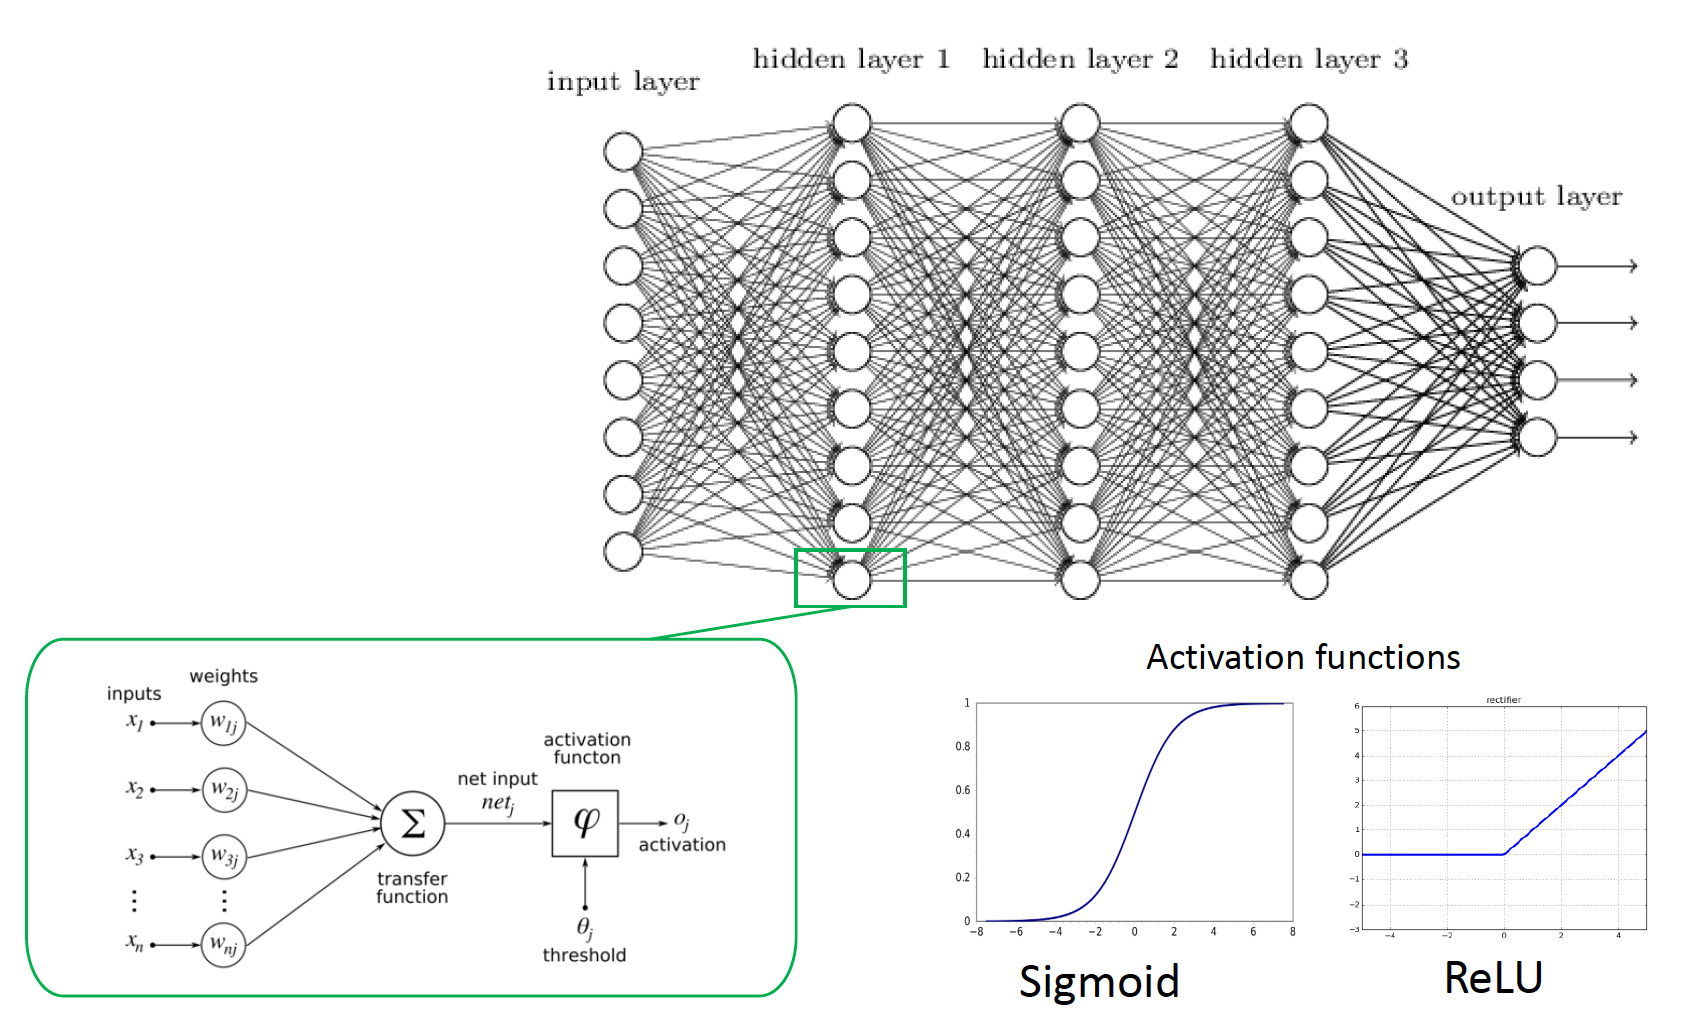
\includegraphics[height=.5\textwidth]{ANN}
%	\end{center}
	
	\item $n_2$-hyperplanes $\theta^{1}(x^1) = W^1 x + b^1$ where $W^1: \mathbb{R}^{n_1} \mapsto \mathbb{R}^{n_2}$:
	$$
	W^1x^1+b^1=
	\begin{pmatrix}
	w^1_1x^1+b^1_1\\
	w^1_2x^1+b^1_2\\
	\vdots \\  
	w^1_{n_2}x^1+b^1_{n_2}
	\end{pmatrix}\quad \mbox{with }\quad 
	W^1=
	\begin{pmatrix}
	w^1_1 \\
	w^1_2 \\
	\vdots \\  
	w^1_{n_2} 
	\end{pmatrix},\ 
	b^1=
	\begin{pmatrix}
	b^1_1\\
	b^1_2\\
	\vdots \\  
	b^1_{n_2}
	\end{pmatrix}
	$$
	\item $n_2$-neurons:
	$$
	x^2=\sigma(W^1x+b^1)
	=\begin{pmatrix}
	\sigma(w^1_1x+b^1_1)\\
	\sigma(w^1_2x+b^1_2)\\
	\vdots \\  
	\sigma(w^1_{n_2}x+b^1_{n_2})
	\end{pmatrix}
	$$
	\item $\cdots$
\end{enumerate} 

\subsection{Definition of deep neural network functions}\label{sec:DNN}
Given $d, k\in\mathbb{N}^+$ and  
$$
n_1,\dots,n_{k}\in\mathbb{N} \mbox{ with }n_0=d, n_{k+1}=1, 
$$
a general DNN function from $\mathbb{R}^d$ to $\mathbb{R}$ is given by
\begin{align*}
f^0(x)   &=\theta^0(x) \\ 
f^{\ell}(x) &= [  \theta^{\ell} \circ \sigma ](f^{\ell-1}(x)) \quad \ell = 1:k \\
f(x) &= f^k(x). 
\end{align*}
The following more concise notation is often used in computer science literature:
\begin{equation}
\label{compress-dnn}
f(x) = \theta^{k}\circ \sigma \circ \theta^{k-1} \circ \sigma \cdots \circ \theta^1 \circ \sigma \circ \theta^0(x),
\end{equation}
here $\theta^i: \mathbb{R}^{n_{i}}\to\mathbb{R}^{n_{i+1}}$ are linear
functions as defined in \eqref{thetamap1}.  Such a DNN is called a
$(k+1)$-layer DNN, and is said to have $k$-hidden layers. The size of
this DNN is $n_1+\cdots+n_k$.

Thus, we have the following connection of neurons and DNN functions
$$
f^k(x) = \theta^{k}(x^k) = \theta^{k} \circ \sigma \circ \theta^{k-1}(x^{k-1}) = [\theta^{k} \circ \sigma ] (f^{k-1}),
$$
or we can see that
$$
x^k = \sigma(f^{k-1}) = \sigma \circ \theta^{k-1} \circ \sigma (f^{k-2}) = [\sigma \circ \theta^{k-1}] (x^{k-1}).
$$
Based on these notation and connections, we have the following definition of
general artificial neural network functions.

Shallow (one hidden layer) neural network functions:
\begin{equation}
\label{NN1}
\dnn(\sigma; n_1) 
=\bigg\{ f^1(x) = \theta^1 (x^1), \mbox{ with } W^\ell\in \mathbb R^{n_{\ell+1}\times
	n_{\ell}}, b^\ell\in\mathbb R^{n_\ell}, \ell=0, 1, n_0=d, n_2 = 1\bigg\}  
\end{equation}
Deep neural network functions:
\begin{equation}
\label{NNL}
\dnn(\sigma; n_1,n_2,\ldots, n_L)=\bigg\{ f^{L}(x) = \theta^L (x^{L}), 
 \mbox{ with } W^\ell\in \mathbb R^{n_{\ell+1}\times
	n_{\ell}}, b^\ell\in\mathbb R^{n_\ell}, \ell=0:L, n_0=d, n_{L+1}=1\bigg\}  
\end{equation}
If we ignore the width (number of neurons) of network functions, we may 
denote the general deep neural network functions with certain layers.

The 1-hidden layer (shallow) neural network is defined as:
\begin{equation}
\dnn=\dnn(\sigma) = \dnn^1(\sigma)
=\bigcup_{n_1\ge 1} \dnn(\sigma;n_1,1)
\end{equation}
Generally, we can define the L-hidden layer neural network as:
\begin{equation}
\dnn^L(\sigma) := \bigcup_{n_1, n_2, \cdots, n_{L}\ge 1} \dnn(\sigma;n_1,n_2,\cdots,n_L, 1).
\end{equation}







\subsection{ReLU DNN}
In this section, we mainly consider a special activation function,
known as the {\it rectified linear unit} (ReLU), and defined as $\rm
ReLU: \mathbb R\mapsto \mathbb R$,
\begin{equation}
\label{relu}
 {\rm ReLU}(x):=\max(0,x), \quad x\in\mathbb{R}. 
\end{equation}
A ReLU DNN with $k$ hidden layers might be written as:
\begin{equation}
\label{relu-dnn}
f(x) = \theta^{k}\circ {\rm ReLU} \circ \theta^{k-1} \circ {\rm ReLU} \cdots \circ \theta^1 \circ {\rm ReLU} \circ \theta^0(x).
\end{equation}

We note that $\rm ReLU$ is a continuous piecewise linear (CPWL) function.
Since the composition of two CPWL functions is still a CPWL
function, we have the following observation~\cite{arora2016understanding}.
\begin{lemma}\label{dnn-cpwl}
	Every ReLU DNN: $\mathbb{R}^d\to\mathbb{R}^c$ is a continuous
	piecewise linear function.  More specifically, given any ReLU DNN,
	there is a polyhedral decomposition of $\mathbb R^d$ such that this
	ReLU DNN is linear on each polyhedron in such a decomposition.
\end{lemma}

Here is a simple example for the ``grid" created by some 2-layer ReLU DNNs in $\mathbb{R}^2$.

\begin{figure}[ht]
	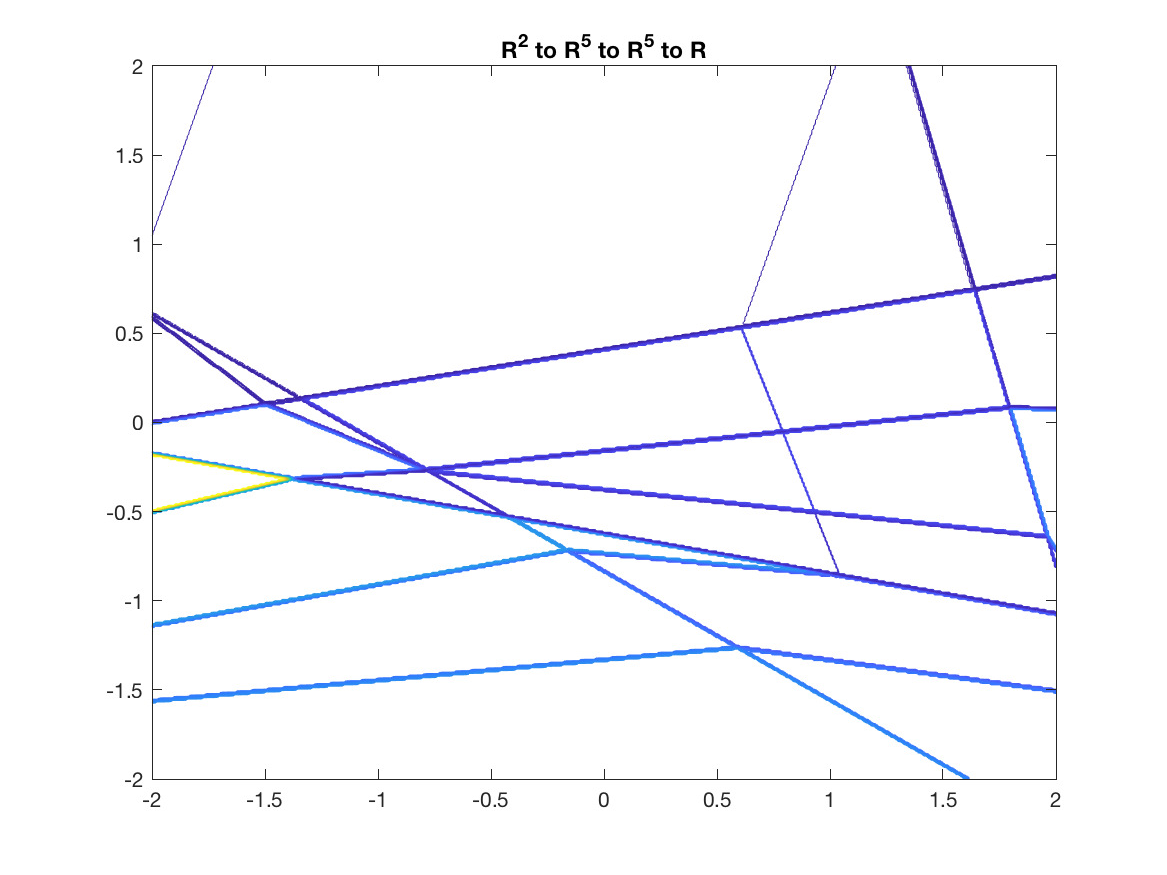
\includegraphics[width=.3\textwidth]{figures/2to5to5to1-eps-converted-to.pdf}  
	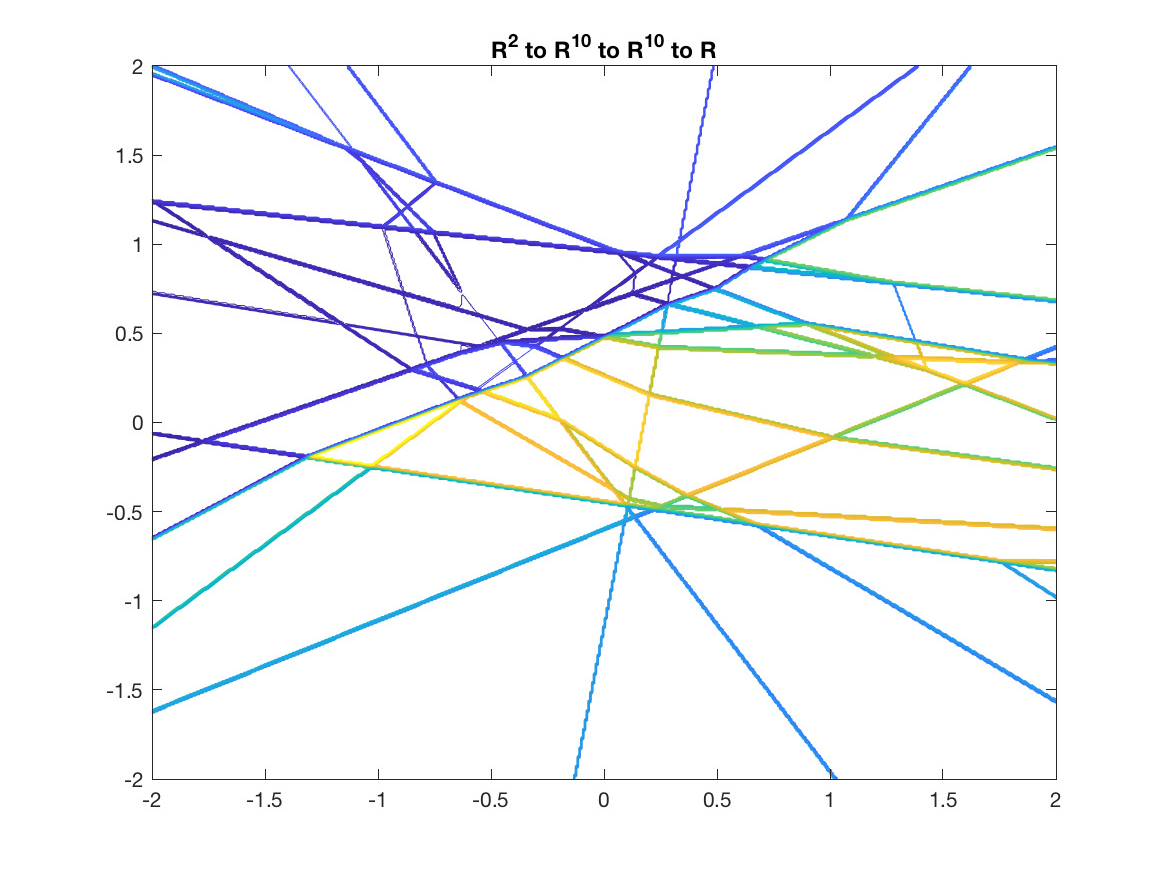
\includegraphics[width=.3\textwidth]{figures/2to10to10to1-eps-converted-to.pdf}  
	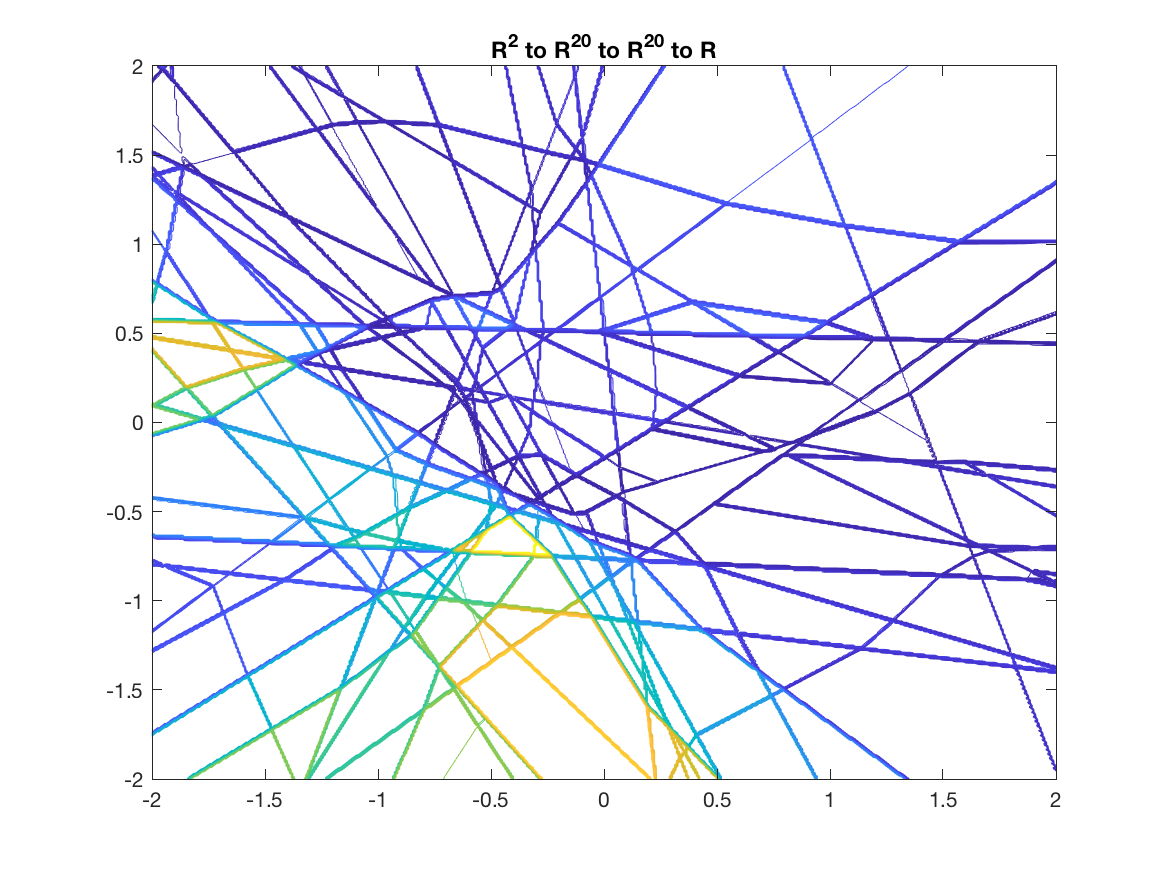
\includegraphics[width=.3\textwidth]{figures/2to20to20to1-eps-converted-to.pdf}  
	\caption{Projections of the domain partitions formed by 2-layer ReLU DNNs with sizes $(n_0, n_1, n_2, n_3)= (2, 5, 5, 1), (2, 10, 10, 1) \text{and}\ (2, 20, 20, 1)$ with random parameters.}
	\label{fig:dnn-region}
\end{figure}

For convenience of exposition,  we introduce the following notation:
%\begin{equation}
%\begin{aligned}
%{\rm{DNN}_L} :=\{& f:f=
%\theta^L \circ {\rm ReLU} \circ \theta^{L-1} \cdots {\rm ReLU}\circ \theta^0(x), \\
%&\theta^\ell \in \mathbb{R}^{n_{\ell} \times (n_\ell+1)}, \quad n^0 = d, \quad n^{L+1} = 1, \quad n^\ell \in \mathbb{N}^+\}.
%\end{aligned}
%\end{equation}
Namely $\dnn^L({\sigma})$ represents the DNN model with $L$ hidden layers and
ReLU activation function with arbitrary size, if $\sigma = {\rm ReLU}$.

 

In this chapter, we will discuss a number of activation functions.  We
say an activation function $\alpha$ 
satisfies the basic activated-approximation-property (AAP) if for any $g\in C^1[-1,1]$, we have
\begin{equation}
\label{AAP}
\min_{a_i,b_i,c,w_i\in\mathbb R^1}\max_{t\in[-1,1]}\bigg|g(t)-\sum_{i=1}^k(a_i\alpha(w_it+b_i)-c\bigg|
\le \frac{C}{k}\max_{t\in[-1,1]}|g'(t)|
\end{equation}
for some constant $C$ independent of $k$ and $g$. 

\section{Cardinal B-splines}
The {\it cardinal B-splines} are given by the following recurrent
relationship
\begin{equation}
  \label{cardinal}
M_d(x)=\frac{x}{d}M_{d-1}(x)  + \frac{d+1-x}{d}M_{d-1}(x-1)  
\end{equation}
\subsection{$d=0$}
\begin{equation}
  \label{cardinal}
M_0(x)=
\left\{
  \begin{array}{ll}
0 & x<0 \\
1 & 0\le x<1    \\
0 & x > 1    
  \end{array}
\right.
\end{equation}
The Heaviside function is defined by
\begin{equation}
  \label{a0}
\alpha_0(x)=
\left\{
  \begin{array}{ll}
0 & x<0; \\
1 & x \ge 1.
  \end{array}
\right.
\end{equation}
\begin{lemma}
  \begin{equation}
  \label{a0M0}
\alpha_0(x)=\sum_{j=0}^\infty M_0(x-j)    
  \end{equation}
  \begin{equation}
  \label{M0a0}
M_0(x)=\alpha_0(x)-\alpha_0(x-1).
  \end{equation}
\end{lemma}

\subsection{$d=1$}
\begin{equation}
  \label{M1M0}
M_1(x)=xM_0(x)+(2-x)M_0(x-1)  
\end{equation}
We note that
\begin{equation}
  \label{M1}
M_1(x)= 
\left\{
\begin{array}{cl}
0 & x<0; \\
x & 0\le x < 1\\
2-x & 1\le x \le 2\\
0 & x>2.
  \end{array}
\right.
\end{equation}
We define (see Fig. \ref{alpha1})
\begin{equation}
  \label{a1}
\alpha_1(x)= 
\left\{
\begin{array}{cl}
M_1(x) &  x < 1\\
1 & x\ge 1
  \end{array}
\right.
\end{equation}
\begin{figure}[!htb]
	\center{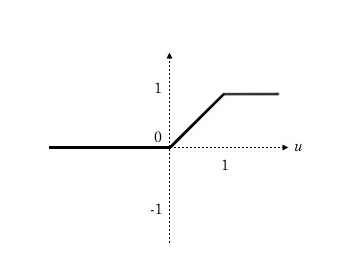
\includegraphics[width=10cm] {figures/alpha1.png}}        
	\caption{The activation $\alpha_1$}      
	\label{alpha1}
\end{figure}
 

\begin{lemma}
  \begin{equation}
    \label{a1a0}
\alpha_1(x)=x\alpha_0(x)+(1-x)\alpha_0(x-1).    
  \end{equation}
\end{lemma}

\begin{lemma}
  \begin{equation}
  \label{a1M1}
\alpha_1(x)=\sum_{j=0}^\infty M_1(x-j)    
  \end{equation}
\end{lemma}

\begin{lemma}
  \begin{equation}
    \label{M1a1}
M_1(x)=\alpha_1(x)-\alpha_1(x-1). 
  \end{equation}
\end{lemma}
Consider the following
$$
\alpha_1(x)-\alpha_1(2x-1). 
$$
We note that the so-called ReLU is defined as follows:
\begin{equation}
  \label{ReLU}
ReLU(x)= 
\left\{
\begin{array}{cl}
0 & x<0; \\
x & x\ge 0
  \end{array}
\right.
\end{equation}
and
\begin{equation}
\alpha_1(x)=ReLU(x)-ReLU(x-1).
\end{equation}

\begin{equation}
\alpha_1({1 \over h_1} x) - \alpha_1({1 \over h_2} (x - h_1) )
\end{equation}




\newpage
\subsection{$d=2$}
\begin{equation}
  \label{M2}
M_2(x)=\frac{x}{2}M_{1}(x)  + \frac{3-x}{2}M_{1}(x-1)   
\end{equation}
Note that
$$
M_2(0)=0, M_2(1)={1\over 2}, M_2({3\over2})={3\over 4},
M_2(2)={1\over2}, M_2(3)=0.
$$
Now we define
\begin{equation}
  \label{a2}
\alpha_2(x)= 
\left\{
\begin{array}{cl}
{4\over3}M_2(x) &  x < {3\over 2}\\
1 & x\ge {3\over2}
  \end{array}
\right.
\end{equation} 
Note that
$$
\alpha_2(0)=0, \alpha_2(1)={1\over 3}, \alpha_2({3\over2})=\alpha_2(2)=\alpha_2(3)=1.
$$
\begin{lemma}
 \begin{equation}
    \label{M2a2}
M_2(x)={3\over 2}(\alpha_2(x)-\alpha_2(x-1)).
  \end{equation}  
\end{lemma}
\begin{proof}
 We need to check some details ...
\end{proof}

\subsection{$d=3$}
The presentation below follows the file lect-spline.pdf found in the following web page
\begin{verbatim}
https://www.geos.ed.ac.uk/~yliu23/docs/lect_spline.pdf
\end{verbatim}
Take $x_0=0$ and $h=1$, we get
$$
B_0(x)=
\left\{
  \begin{array}{ll}
0 & x\le -2\\
\\
{1\over 6}(2+x)^3 & -2\le x\le -1\\ 
\\
{2\over 3}-{1\over2}x^2(2+x) & -1\le x\le 0\\  
\\
{2\over 3}-{1\over2}x^2(2-x) & 0\le x\le 1\\  
\\
{1\over 6}(2-x)^3 & 1\le x\le 2\\ 
\\
 0 & x\ge 2.    
  \end{array}
\right.
$$
Let 
$$
B_k(x)=B_0(x-k)
$$
A cubic spline function in $[0,N]$ can be written as
$$
S(x)=\sum_{k=-1}^{N+1}a_kB_0(x-k).
$$
The following identity holds:
\begin{equation}
  \label{eq:1}
\sum_{k=-1}^{N+1}B_0(x-k) =1, \quad\forall x\in [0,N]
\end{equation}
We propose the following activation function
$$
\sigma(x)=
\left\{
  \begin{array}{ll}
B_1(x) & x\le 1 \\
1 & x\ge 1    
  \end{array}
\right.
$$


\section{Approximation properties}
We consider an interval $I =(0,1)$ and a partition
\begin{equation}
  \label{1d-partition}
-1=t_0  < t_1<\ldots<t_k=1.
\end{equation}
As a special case of uniform partition, we take
\begin{equation}
\label{tk}
t_i=t_0+ih, I_i=(t_{i-1}, t_i)\quad i=1:k, h={2\over k}.  
\end{equation}
Consider the basis function 
$$
M_{0,i}(t)=M_0(\frac{t-t_{i-1}}{h}).
$$
Given 
$$
v: (-1,1)\mapsto \mathbb R^1
$$
The interpolation is defined as
\begin{equation}
  \label{interp0}
(\Pi_0v)(t) =\sum_{i=1}^kv_iM_{0,i}(t)
=v_1+\sum_{i=2}^k(v_i-v_1)M_{0,i}(t)
\end{equation}
with 
$$ 
v_i={1\over h}\int_{I_i}v(t).
$$
By \eqref{M0a0}, we have
\begin{eqnarray}
(\Pi_0v)(t)
&=&v_1+\sum_{i=2}^k(v_i-v_1)(\alpha_{0}(\frac{t-t_{i-1}}{h})-\alpha_{1}(\frac{t-t_{i}}{h}))\\
&=&v_1+\sum_{i=2}^k(v_i-v_1)(\alpha_{0}(\frac{t-t_{i-1}}{h})-\alpha_{0}(\frac{t-t_{i}}{h}))\\
&=&v_1+\sum_{i=1}^{k-1}(v_{i+1}-v_1)\alpha_{0}(\frac{t-t_{i}}{h})-
\sum_{i=2}^k(v_i-v_1)\alpha_{0}(\frac{t-t_{i}}{h})\\
&=&v_1+\sum_{i=1}^{k}(v_{i+1}-v_i)\alpha_{0}(\frac{t-t_{i}}{h}).
\end{eqnarray}
with 
$$
v_{k+1}=v_{1}.
$$
\begin{theorem}
  \label{M0-error}
  \begin{equation}
  \label{Pi0-error}
\|v-\Pi_0v\|_{0,\infty}\le \frac{c_0}{k}\|v'\|_{0,\infty}
\end{equation}
\end{theorem}
\begin{proof}
Easy.   
\end{proof}
In general, we consider the following space of Splines:
\begin{theorem}  \label{Md-error}

\subsection{General $d$}
Let $S^{d,k}$ be the spline space generated by the B-spline $M_d$ from
the partition \eqref{1d-partition}, we have
  \begin{equation}
  \label{Pid-error}
\|v-\Pi_{d,k}v\|_{0,\infty}\le \frac{c_d}{k^r}\|v^{(r)}\|_{0,\infty},
\quad 1\le r\le d+1.
\end{equation}
\end{theorem}
\begin{proof}
	You can find this proof in \cite{de1978practical} in theorem $XII.3$ in page 176.
It needs to be checked.  Li Lin might know where a proof can be found
in the literature. 
\end{proof}

\subsection{Sigmoidal function}
The so-called sigmoidal function is defined as follows:
\begin{equation}
  \label{sigmoidal}
\sigma(t) = \frac{1}{1 + e^{-t}}.  
\end{equation}
This popular activation provides a smooth approximation of the Heaviside function $\alpha_0$ as follows:
\begin{equation}
  \label{sig}
\lim_{a\to \infty}\sigma(at) = \alpha_0(t), \quad t\neq 0.
\end{equation}
For $t>0$
$$
\alpha_0(t)- \sigma(at)
=1-\frac{1}{1+e^{-at}}\le e^{-at}.
$$
For $t<0$
$$
\sigma(at)-\alpha_0(t)
=\frac{1}{1+e^{-at}}\le e^{-a|t|}.
$$
We have in general 
$$
|\sigma(at)-\alpha_0(t)|
\le e^{-a|t|}.
$$
We consider the following interpolation 
\begin{equation}
  \label{interp0-1}
v(t)=v_1+\sum_{i=1}  (v_i-v_1)
\end{equation}



%\newpage
\section{Special activation functions}

        \begin{itemize}
	\item An general activation function(must be nonlinear) is 
$$\sigma: \mathbb{R} \to  \mathbb{R}.$$

\item The Heaviside function is 
$$
H(x ) = \begin{cases}
0 \quad &\text{if} ~ x \le 0, \\
1 \quad &\text{if} ~ x > 0.
\end{cases}
$$
The biggest problem for this activation function is that this function is not continuous which will cause 
huge difficult in training phase.

\item The sigmoid function:
$$s(x) = \frac{1}{1 + e^{-x}}
\rightarrow 
\begin{cases}
0,~~x\rightarrow -\infty,\\
1,~~x\rightarrow +\infty.
\end{cases}
.
$$
This function can be seen as the smooth approximation of Heaviside function.
This activation function was very popular in shallow neural network in about 1990s. Now, this
activation function is also often used in RNN or some NLP tasks.


\item Currently, the most used activation function in DNN  and CNN is ``Rectified Linear Unit'' (ReLU):
$$
{\rm ReLU}(x) = \max(0, x).
$$
There are many interesting properties of ${\rm ReLU}$ function:
\begin{enumerate}
	\item ${\rm ReLU}$ is a piecewise linear function. Thus, DNN with this activation 
	function is always a piecewise linear function.
	
	\item The connection of ${\rm ReLU}$ and Heaviside.
	\begin{equation}
	\frac{d}{dx} {\rm ReLU}(x) = H(x).
	\end{equation}
	
	\item Recently, there are huge research works about the approximation properties of DNN
	with ${\rm ReLU}$ activation function see ~\cite{he2018relu,wang2018exponential,yarotsky2017error}.
\end{enumerate}
	
	\item The new activation function from ReLU is:
	$$
	\tau(x) = r(x) - r(x-1) = \begin{cases}
	0 \quad &\text{if} ~ x \le 0, \\
	x \quad &\text{if} ~  0 < x \le 1, \\
	1  \quad &\text{if} ~ x > 1.
	\end{cases}
	$$
        Here we need to note that, because $-r(x) \neq r(ax + b)$, so
        if we use $\tau$ as $f_{out}$, the layers will be $J+1$ for
        ReLU as activation function and $f_{out} = id$.
	\end{itemize}

Here is a simple diagram for a general DNN structure:
\begin{figure}[!h]
	\center{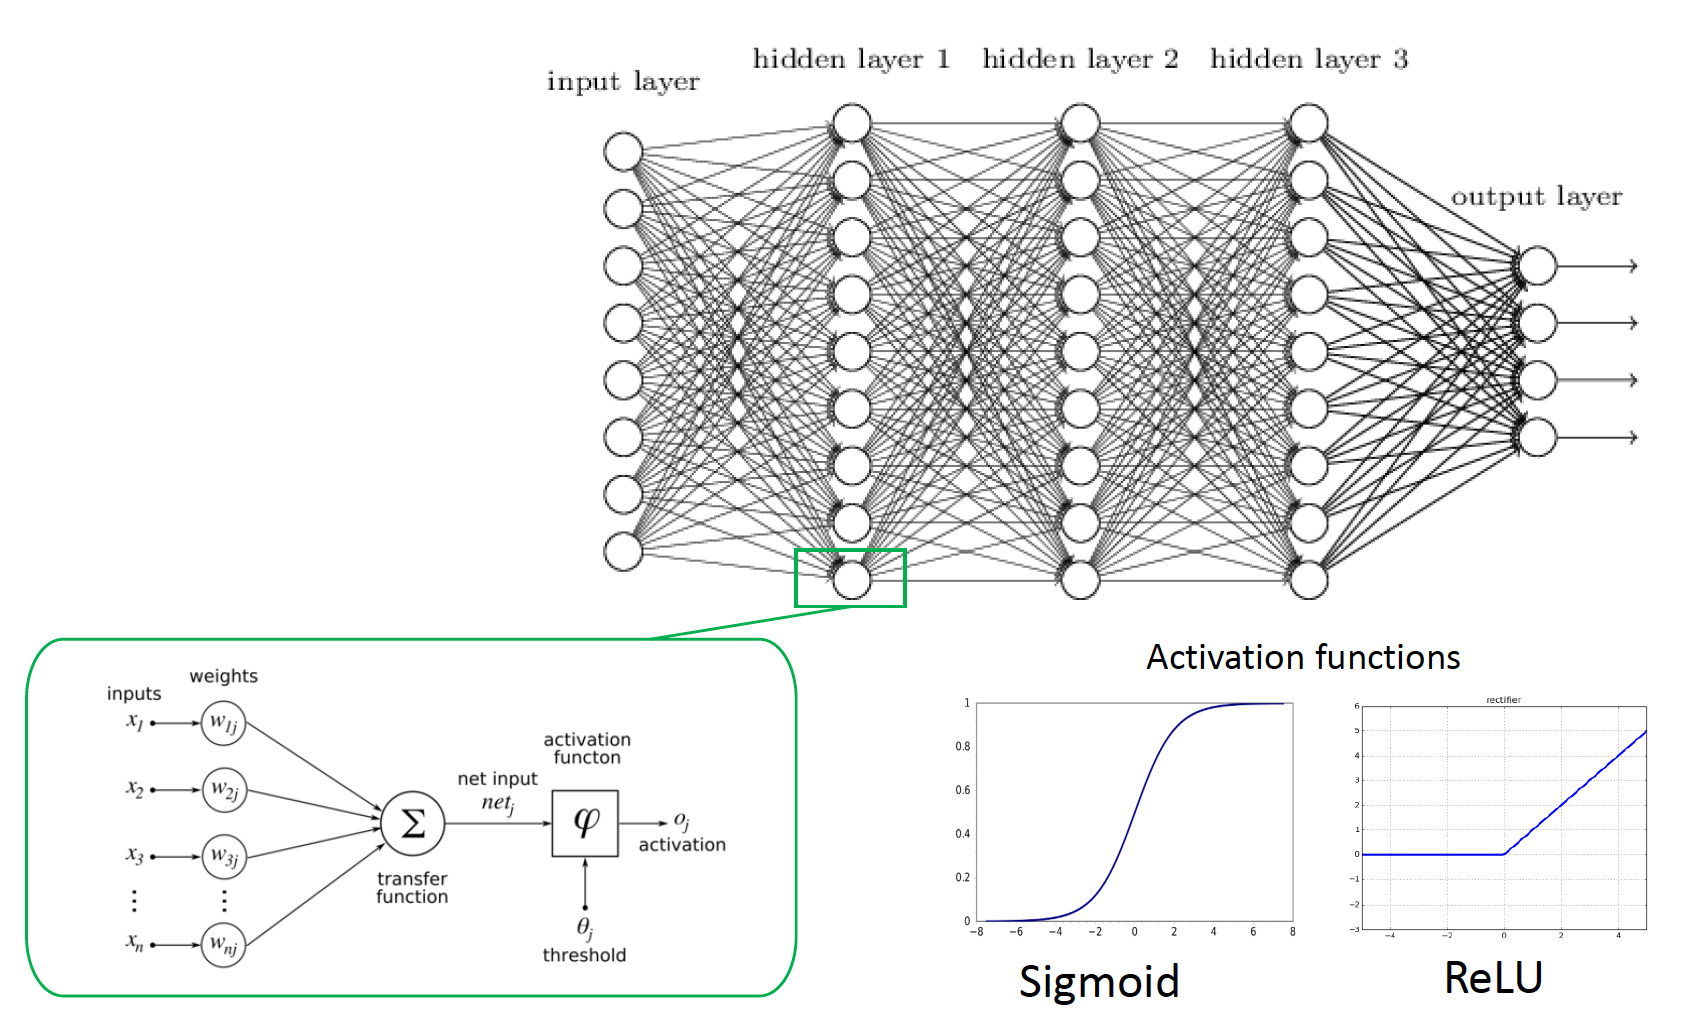
\includegraphics[width=12cm,height=6cm] {ANN.png}}
	\caption{A General Structure of DNN}
\end{figure}



\chapter{Continuous Piecewise Linear Functions and DNN}
%\input{3FEM/linearFE}

\section{General continuous piecewise linear functions as a DNN}
\subsection{Lattice representation of CPWL}

We say a function $f:\mathbb{R}^n \to \mathbb{R}$ is continuous piecewise linear (CPWL) if there exists a finite set of polyhedra whose union is $\mathbb{R}^n$, and $f$ is affine linear over each polyhedron (note that the definition automatically implies continuity of the function because the affine regions are closed and cover $\mathbb{R}^n$, and affine functions are continuous). The number of pieces of $f$ is the number of maximal connected subsets of $\mathbb{R}^n$ over which $f$ is affine linear (which is finite).

\begin{figure}[!ht]
\centering
	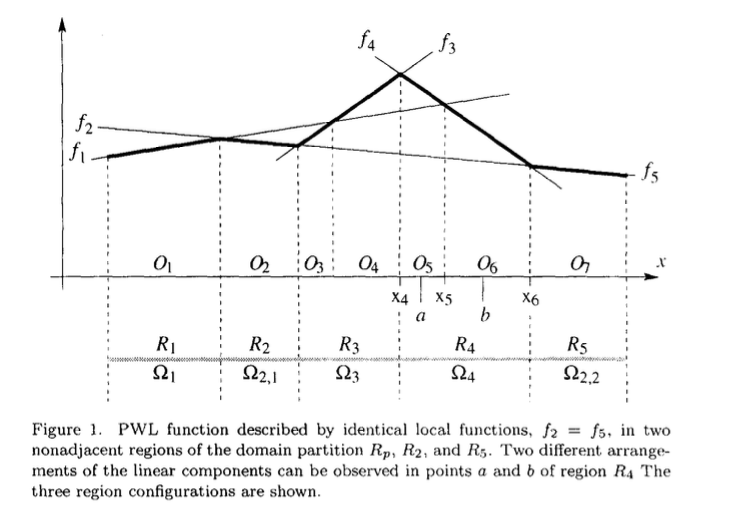
\includegraphics[width=0.6\textwidth]{6DL/figures/latticePWL.png}   
	\caption{Unique order regions.} 
	\label{fig:latticePWL}
\end{figure}
Figure \ref{fig:latticePWL} shows a CPWL function with unidimensional domain that has a domain partition generated by $4$ boundaries. The result is a set of $5$ regions and the corresponding set of $5$ local functions, two of which are identical, $f_2$ and $f_5$. In the case of a model described in terms of the local functions. 

The arrangements in ascending order of the linear functions in the points $a$ and $b$ of region $R_4$ are respectively, ($f_2 = f_5 < f_1 < f_4 < f_3$) and ($f_2= f_5 < f_4 < f_1 < f_3$). We note that the intersection of the linear functions fland f4occurs at point x5, an inner point of $R_4$. Given the importance of the order arrangement when dealing with models based on the local functions, the division of region $R_4$ into two subregions is practically meaningful.

Any intersection of linear functions produces a change of order arrangement. So, if we consider every intersection of local functions, the resulting domain partition will be formed by connected, and convex regions with a unique order arrangement. It should be noted that some of those intersections might not correspond to any boundary of the PWL function.  

We introduce a domain partition that will have unique order on each subdomain \cite{tarela1999region}.
\begin{definition}
	Let $f:\mathbb{R}^n\to\mathbb{R}$ be a continuous piecewise linear function with m distinct local functions $l_i$, $1\le i\le m$. Consider the intersections between local functions, those intersections with some noticed segments in $f$ will be called visible boundaries, and those boundaries corresponds to the set of functions $\{\phi_{\lambda_v}\}$. The rest of intersections occurring inside the domain will be called hidden boundaries and noted as $\{\phi'_{\lambda_h}\}$. A \textbf{unique-order region} is each region of the domain partition produced by the boundary configuration $\{\phi_{\lambda_v}\}\bigcup\{\phi'_{\lambda_h}\}$.
\end{definition}

\bigskip
The unique-order regions have the following characterizations:
\begin{itemize}
	\item The domain of $f$ is divided into $M$ unique-order regions.
	\item The local function associated to two unique-order regions may be identical.
	\item The unique-order regions are convex.
	\item A unique-order region has the same rearrangement in ascending order of the values of the $m$ local functions in all its points.
\end{itemize}

\begin{remark}
	If $m$ is the number of distinct linear components of $f$, then the maximum number of rearrangements in ascending order is $m!$. However, the number of unique-order regions is in general lower than $m!$, because of the geometric constraints of the problem \cite{wilkinson1963method}. Thus, the different arrangements in $\mathbb{R}^n$ is $Q$, then:
	\begin{equation*}
	\begin{aligned}
	&\mathrm{if}\ 1\le m\le n+1\quad\Rightarrow Q=m!\\
	&\mathrm{if}\ m\ge n+2\quad\Rightarrow (n+1)!<Q<m!
	\end{aligned}
	\end{equation*}
	The number of unique-regions is $M$, then we have $M\le Q$, since only some of these arrangements constitute unique-order regions.
\end{remark}




\begin{lemma}\label{lem:1dlattice}
	If $p(t)$ is a continuous piecewise linear function. And the unique-order region partition is
	$$0 = t_0 < t_1 < ... < t_{r+1} = 1$$
	and the linear function in $[t_i,t_{i+1}]$ is $l_i(t) = k_i t+b_i$. And parameter satisfied 
	$$ b_0 > b_r,\qquad k_0 + b_0 > k_r + b_r $$
	which means
	$$l_0(t)> l_r(t)\quad \mbox{in}\quad [t_0,t_1]$$
	$$l_0(t)> l_r(t)\quad \mbox{in}\quad [t_r,t_{r+1}]$$
	Then, exist $l_p(t) = k_p t+ b_p$, such that
	$$b_p \ge b_0,\qquad k_p+b_p\le k_r+b_r$$  
	That's to say
	$$l_0(t)\le l_p(t)\quad \mbox{in}\quad [t_0,t_1]$$
	$$l_p(t)\le l_r(t)\quad \mbox{in}\quad [t_r,t_{r+1}]$$
\end{lemma}
\begin{figure}[th]
	\centering
	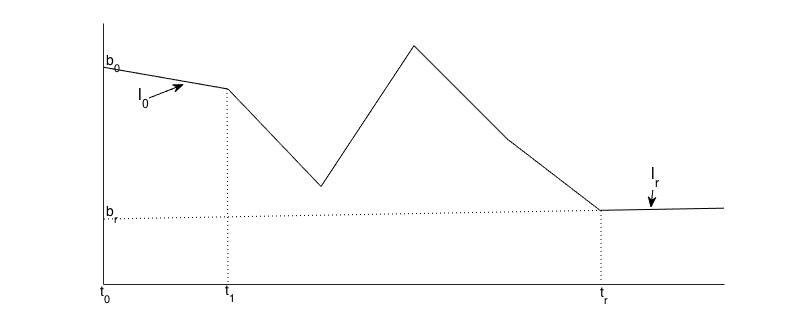
\includegraphics[width=0.7\linewidth]{6DL/pic/fig1}
	\caption{}
\end{figure}

\begin{proof}
	
	Let $k_p=\min\{k_i\}$, $\Delta t_i=t_{i+1}-t_i$. 
	Since here we only have linear functions, so we can represent each point $(t_i,y_i)$ by using $k_i$'s and $\Delta t_i$'s.
	Then the point $(t_p,b_0+\sum_{i=0}^{p-1}k_i\Delta t_i)$ is on $y=k_p t+b_p$, so we can represent $b_p$ as following:
	$$b_p=b_0+\sum_{i=0}^{p-1}k_i\Delta t_i-k_p t_p=b_0+\sum_{i=0}^{p-1}(k_i-k_p)\Delta t_i$$
	Since here $k_p$ is the minimum, we have:
	$$b_p=b_0+\sum_{i=0}^{p-1}(k_i-k_p)\Delta t_i\ge b_0$$		
	And
	\begin{equation*}
	\begin{aligned}
	k_p+b_p&=k_p+b_0+\sum_{i=0}^{p-1}(k_i-k_p)\Delta t_i\\
	k_r+b_r&=k_r+b_0+\sum_{i=0}^{r-1}(k_i-k_p)\Delta t_i\\
	(k_r+b_r)-(k_p+b_p)&=k_r-k_p+\sum_{i=p}^{r-1}(k_i-k_p)\Delta t_i\ge 0
	\end{aligned}
	\end{equation*}
	which means we find the desired pair of $k$ and $p$.
	Notice here $k_p\ne k_0$ and $k_p\ne k_r$ by the assumptions in the lemma. This completes the proof.
	
\end{proof}	


\bigskip		
\begin{theorem}\label{PWLtoRelu}
	For every continuous piecewise linear function $f:\mathbb{R}^n\to\mathbb{R}$ with finite pieces defined by the distinct local linear functions $l_i$, $1\le i\le m$ and $\{\Omega_k\}_{k=1}^M$ be the unique-order subdomains. Then there exist finite non-empty subsets of $\{1,2,\dots,m\}$, say $s_k$, $1\le k\le M$, such that 
	\begin{equation}
	f(x)=\max_{1\le k\le M}\{\min_{i\in s_k} l_i\},
	\end{equation}
	here $s_k=\{i: l_i\ge l_k\ \mathrm{on}\ \Omega_{k}\}$.
\end{theorem}


\begin{proof}
	Let $l_i(x)=f(x)|_{\Omega_k}$. In each $\Omega_{k}$, consider the functions lie completely above $l_k$, and define the convex polynomial
	$$\Phi_{k}=\min_{i\in s_k} l_i.$$
	Define
	$$\Phi(x)=\max_{k} \Phi_{k}(x)$$
	and next we show that $\Phi_{k}(x)\le f(x)$ for all x and every $k$.
	 
	
	For any fixed $k$, if $x_0\in\Omega_{k}$,
	$$
	\Phi_{k}(x_0)=l_k(x_0)= f(x_0).
	$$
	If $x_0\notin\Omega_{k}$, then we suppose $x_0\in \Omega_{k'}$, so 
	$$
	f(x_0)|_{\Omega_{k'}}=l_{k'}(x_0).
	$$ 
	Notice that here we have unique-order region, thus in each $\Omega_i$, the order of $l_k$ and $l_{k'}$ is fixed. There're several situations:
	\begin{enumerate}
		\item  If $l_{k'}(x)\ge l_{k}(x)$ for $x\in \Omega_{k}$, then $l_{k'}$ is a lattice variable in the convex polynomial $\Phi_k$, and so
		$$\Phi_{k}(x_0)\le l_{k'}(x_0)=f(x_0).$$
		\item  If $l_{k'}(x)< l_{k}(x)$ for $x\in \Omega_{k}$, then we consider the domain $\Omega_{k'}$:
		\begin{enumerate}
			\item 
			If $l_{k'}(x)\ge l_k(x)$ for $x\in \Omega_{k'}$. Then on $\Omega_{k'}$,
			\begin{equation*}
			\Phi_{k}(x_0)= l_k(x_0)\le l_{k'}(x_0)=f(x_0)
			\end{equation*}
			\item  
			If $l_{k'}(x)< l_k(x)$ for $x\in \Omega_{k'}$. We take $x\in \Omega_{k}^\circ, x' \in \Omega_{k'}^\circ$. Then we have a path $L(\theta)$, the coordinate of the path is defined as 
			$$
			(x + \theta(x'-x),f(x + \theta(x'-x)))
			$$ 
			with $\theta\in[0,1]$(see Figure~\ref{fig:sec:lattice}). It is just a piecewise linear function with the parameter $\theta$. Notice that the domain partition is unique-order. So if we want to compare the order of the linear function,  we just compare one point value in that region. 
		\begin{figure}[th]
			\centering
			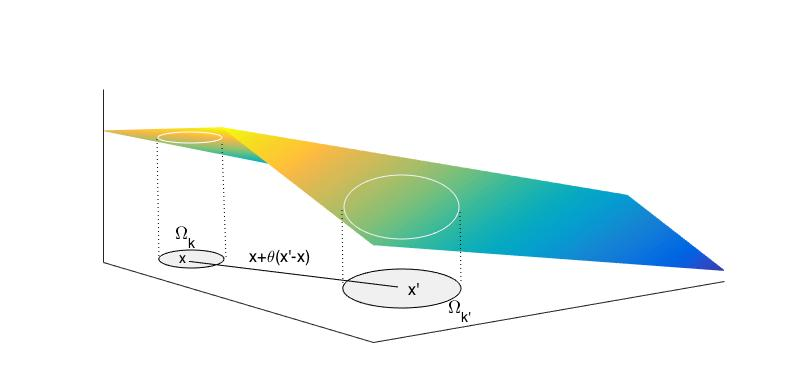
\includegraphics[width=0.7\linewidth]{6DL/pic/fig2}
			\caption{figure}
			\label{fig:sec:lattice}
		\end{figure}
		Then by Lemma \ref{lem:1dlattice}, there must exist $l_t$ with $t\ne k,k'$ and
			\begin{equation*}
			\begin{aligned}
			&l_t\le l_{k'}\quad \mathrm{on}\ \Omega_{k'}\\
			&l_t\ge l_{k}\quad \mathrm{on}\ \Omega_{k}
			\end{aligned}
			\end{equation*}
			Then we should have:
			$$\Phi_{k}(x_0)\le l_t(x_0)\le l_{k'}(x_0)=f(x_0).$$
		\end{enumerate}
	\end{enumerate}
Thus for every $\Phi_{k}$, we have $\Phi_{k}(x)\le f(x)$ for all $x$. It is obvious that  $f(x)\le \Phi_{k}(x)$ for all $x$ since
$$
f(x)=l_k(x)\le \max_k l_k=\max \Phi_k=\Phi(x),\quad \forall x\in \Omega_k.
$$
So 
			$$f(x)=\max_{k}\min_{i\in s_k}\{l_i\}$$
			This is exactly the desired form. Here $|s_k|\le m$, and the number of $\Phi_{k}$ depends on the partition we do. 
\end{proof}




\subsection{General CPWL as a DNN}

Assume that $f:\mathbb{R}^d\to\mathbb{R}$ is a continuous function
that are piecewise linear on $m$ subdomains
$$
\Omega_i, \quad i=1:m.
$$
Namely, on each $\Omega_i$, $f$ is a linear function:
$$
f(x)=f_i(x)=a_i\cdot x+b_i, \quad x\in \Omega_i,
$$
with some $a_i \in \mathbb{R}^d$ and $b_i \in \mathbb{R}$.

Combining Theorem \ref{PWLtoRelu} with Lemma \ref{linearcombine2Relu}, we have the following result.
\begin{theorem}
Every $\mathbb{R}^{d} \rightarrow \mathbb{R}$ ReLU DNN represents a piecewise linear function, and every piecewise linear function $\mathbb{R}^{d} \rightarrow \mathbb{R}$ can be represented by a ReLU DNN with at most $\left\lceil\log _{2}(d+1) \right\rceil+1$ depth.
\end{theorem}
\begin{proof}
It is clear that any function represented by a ReLU DNN is a PWL function. To see the converse, we first note that any PWL function can be represented as a linear combination of piecewise linear convex functions. More formally, by Theorem \ref{PWLtoRelu}, for every piecewise linear function $f: \mathbb{R}^{d} \rightarrow \mathbb{R},$ there exists a finite set of affine linear functions $\ell_{1}, \ldots, \ell_{m}$ and subsets $s_{1}, \ldots, s_{M} \subseteq\{1, \ldots, m\}$ (not necessarily disjoint) where each $s_{i}$ is of cardinality at most $d+1,$ such that
$$
f=\sum_{k=1}^{p} v_{k}\left(\max _{i \in s_{k}} \ell_{i}\right)
$$
where $v_{j} \in\{-1,+1\}$ for all $j=1, \ldots, p .$ Since a function of the form $\max _{i \in s_{j}} \ell_{i}$ is a piecewise linear convex function with at most $n+1$ pieces (because $\left|s_{j}\right| \leq d+1$ ),   any continuous piecewise linear function (not necessarily convex) can be obtained as a linear combination of piecewise linear convex functions each of which has at most $d+1$ affine pieces. Note that $\max \{x, y\}=\frac{x+y}{2}+\frac{|x-y|}{2}$ is implementable by a two layer ReLU network and use this construction in an inductive manner to show that maximum of $d+1$ numbers can be computed using a ReLU DNN with depth at most $\left\lceil\log _{2}(d+1)\right\rceil$.
\end{proof}


For the relationship between ReLU DNNs and general CPWL functions, we have the next theorem with some estimation~\cite{arora2016understanding}. 
\begin{theorem}\label{main0}
	A continuous function $f:\mathbb{R}^d\to\mathbb{R}$ that are piecewise linear on $m$ subdomains $\{\Omega_j\}_{j=1}^m$ can be represented by a ReLU DNN. 
	Furthermore, 
	\begin{enumerate}
		\item the number of  hidden layers  is bounded by 
		\begin{equation}
		\label{layer}
		N_{\rm layer}\le \lceil \log_2(d+1)\rceil.      
		\end{equation}
		\item the number of neurons 
		\begin{equation}
		\label{neurons}
		N_{\rm neuron}=
		\left\{
		\begin{array}{ll}
		\mathcal  O\left(d2^{mM+(d+1)(m-d-1)}\right) & \mbox{ if } m\ge d+1,\\     
		\mathcal O\left(d2^{mM}\right) & \mbox{ if } m< d+1.
		\end{array}
		\right.
		\end{equation}
		here $M$, satisfying $m\le M\le m!$, is the number of subdomains in which $f_i-f_j$ does not change sign. 
	\end{enumerate}
\end{theorem}
Combining Theorem~\ref{main0} with Theorem~\ref{lowerbound}, we have the following corollary regarding the minimal number of layers needed to recover all piecewise linear functions.

\begin{corollary}
	\begin{equation}
	2 \le J_d \le \lceil\log_2(d+1)\rceil.
	\end{equation}
	This also indicates that $\lceil\log_2(d+1)\rceil$ is ``optimal" for $d=2,3$.
\end{corollary}



\endinput 

\section{$\lceil \log(d+1)\rceil$-depth dnn}
Given any $L>n+1$ linear functions, the maximum of these $L$ functions can be represented as the maximum of only $n+1$ linear functions. The next lemma shows that we can reduce the number of functions by one if it is larger than $n+1$. 
Let $l(x,a)=[1\ x^T]a$.
\begin{lemma}\label{reduce}
	For any interger $L$ with $1\le n< L$, $c_0\in\mathbb{R}$ and arbitrary linear function $l_1(x),\dots,l_L(x)$ of $x\in\mathbb{R}^d$, there exist finite groups of $L-1$ linear functions, say $l(x,b_1(k))$, $\dots$,
	$l(x,b_{L-1}(k))$, $1\le k\le K$, and corresponding $c_k\in\mathbb{R}$, $\sigma_k\in\{1,-1\}$ such that
	
	\begin{equation}\label{goal}
	\max\{c_0,l_1,\dots,l_L\} = \sum_{k=1}^{K}\sigma_k\max\{c_k,l(x,b_1(k)),\dots,l(x,b_{L-1}(k))\},
	\end{equation}
	where $K=2^{n+1}-1$.
\end{lemma}

\begin{proof}
		Let $l_i(x)=l(x,a_i)=a_{i0}+x^T\bar{a}_i$ with $a_{i0}\in\mathbb{R}$ and $\bar{a}_i\in\mathbb{R}^n$ for $1\le i\le L$. Assume there are at most $\bar{n}$ linearly independent $\bar{a}_i$, $\bar{n}\le n$. Without loss of generality, assume $\bar{a}_1,\dots,\bar{a}_{\bar{n}}$ are linearly independent. Then by basic linear algebra, we know that 
		\begin{equation}\label{0}
		l_L=\sum_{j=1}^{\bar{n}}\alpha_j l_j+\alpha_0.
		\end{equation}
		Denote
		$$
		\mu(x)=\max\{l_{\bar{n}+1},\dots,l_{L-1}\}.
		$$
		Then
		\begin{equation}\label{1}
		\max\{c_0,l_1,\dots,l_L\}=\max\{c_0,l_1,\dots,l_{\bar{n}},\mu(x),l_L\}.
		\end{equation}
		 If $\alpha_j = 0$ in \eqref{0} for each $1\le j\le \bar{n}$, then by taking $\max\{c_0,\alpha_0\}$, we already make the RHS of (\ref{1}) as the RHS of (\ref{goal}). Otherwise, $\exists \alpha_j\ne0$ for some $1\le j\le \bar{n}$, we can assume that $\alpha_{\eta} \neq 0, \alpha_{\eta+1}= ... = \alpha_{\bar{n}}=0$, so 
		$$
		l_L=\sum_{j=1}^{\eta}\alpha_j l_j+\alpha_0,\qquad \eta\le \bar{n}.
		$$ 
		Next we show that it can be represented by
		\begin{equation}\label{latticereaarange1}
		\max\{c_0,l_1,\dots,l_L\}=\max\{c_0,l_1',\dots,l_{\bar{n}}',\mu(x),l_L'\}
		\end{equation}
		where $\displaystyle l_L'=\alpha_\eta l_\eta+\sum_{j=1}^{\eta-1}\alpha_jl_j'+\alpha_0$ with $\alpha_\eta\neq 1$.
		
		If $\alpha_i=1$ for each $1\le i\le\eta$, we can do the following linear transformation $(l'_1,\dots,l'_{\bar{n}})^T=A(l_1,\dots,l_{\bar{n}})^T$, where
		\begin{equation*}
		\begin{aligned}
		l'_i&=l_i,\qquad &\mathrm{for}\ i\ne\eta,\\
		l'_i&=\sum_{j=1}^{\eta} l_j+\alpha_0,\qquad &\mathrm{for}\ i=\eta.\\
		\end{aligned}
		\end{equation*} 
		Then (\ref{1}) equals 
		$$
		\max\{c_0,l'_1,\dots,l'_{\bar{n}},\mu(x),-\alpha_0-l'_1-\dots-l'_{\eta-1}+l'_{\eta}\}.
		$$
		in this case, 
		$$
		l_L'=-\alpha_0-l'_1-\dots-l'_{\eta-1}+l'_{\eta}
		$$
		the coefficients of $l'_1,\dots,l'_{\eta-1}$ are not 1. So we can rearrange $l_i'$ and assume there is at least one $\alpha_i\ne1$ for $1\le i\le\eta$, say $\alpha_{\eta}\ne1$. This leads to the representation \eqref{latticereaarange1}. Let
		\begin{equation*}
		\begin{aligned}
		f&=\max\{c_0,\mu(x),l_1',\dots,l_{\eta-1}',l_{\eta+1}',\dots,l_{\bar{n}}'\},\\
		g&=l_{\eta},\\
		h&=\sum_{j=1}^{\eta-1}\alpha_j l_j'+\alpha_0.
		\end{aligned}
		\end{equation*}
		By (\ref{key-reduce}), 
		\begin{eqnarray}\label{2}
		\max\{c_0,l_1',\dots,l_{\bar{n}}',\mu(x),l_L'\}&&=\max\{f,g,\alpha_{\eta} g+h  \}\\ 
		\label{3}
		&&=\sigma_1\max\{f,g,\frac{\sum_{j=1}^{\eta-1}\alpha_j l_j'+\alpha_0}{1-\alpha_{\eta}}  \}\\ 
		\label{4}
		&&+\sigma_2\max\{f,\alpha_{\eta} g+h,\frac{\sum_{j=1}^{\eta-1}\alpha_j l_j'+\alpha_0}{1-\alpha_{\eta}}   \}\\ 
		\label{5}
		&&+\sigma_3\max\{f,\bar{g} \}.
		\end{eqnarray}
		(\ref{5}) is already the desired form, because now we only take maximum  over $L-1$ linear functions and one constant.
		
		As for the (\ref{3}), notice that now we have eliminated $l_{\eta}$ in the third expression
		$$
		\alpha_\eta l_\eta'+\sum_{j=1}^{\eta-1}\alpha_j l_j'+\alpha_0\quad \Rightarrow \quad \frac{\sum_{j=1}^{\eta-1}\alpha_j l_j'+\alpha_0}{1-\alpha_{\eta}}.
		$$ 
		So continue this procedure, at last we will only have constant in the last expression, by taking maximum of this constant and $c_0$, we can reduce one term in the max expression.
		
		For (\ref{4}), consider the linear transformation $(l''_1,\dots,l''_{\bar{n}})^T=B(l_1',\dots,l_{\bar{n}}')^T$:
		\begin{equation*}
		\begin{aligned}
		l''_i&=l_i',\qquad &\mathrm{for}\ i\ne\eta,\\
		l''_i&=\sum_{j=1}^{\eta}\alpha_{j} l_j'+\alpha_0,\qquad &\mathrm{for}\ i=\eta.\\
		\end{aligned}
		\end{equation*}
		So (\ref{4}) becomes
		$$
		\max\{c_0,\mu,l''_1,\dots,l''_{\bar{n}},\sum_{j=1}^{\eta-1}\alpha_j l''_j+\alpha_0\}.
		$$
		Then it is the same as (\ref{3}). Follow the same steps as for \eqref{3}, we can achieve the desired result.
	\end{proof}
	
	\begin{figure}[ht]
		\begin{center}
			\begin{tikzpicture}[>=triangle 45,font=\sffamily]
			\node (X)  {(\ref{2})};
			\node (Y) [below left=1cm and 2cm of X]  { (\ref{3})};% 2cm below, 1cm to the left (optional)
			\node (Z) [below right=1cm and 2cm of X] {(\ref{4})};
			\node (O) [below =1 cm of X] {(\ref{5})};
			\node (U) [below left=1cm and 1.2cm of Y] { ...};
			\node (V) [below right=1cm and 1.2cm of Y] {... };
			\node (W) [below =1cm of Y] { };
			\node (U1)[below left=1cm and 1.2cm of Z] {...};
			\node (V1)[below right=1cm and 1.2cm of Z] {...};
			\node (W1) [below =1cm of Z] {};
			\node (T1)[below left=1cm and 0.5cm of U] { };
			\node (T2)[below right=1cm and 0.5cm of U] { };
			\node (T3)[ below =1cm of U] { };
			\node (T4)[ below left=1cm and 0.5cm of V] { };
			\node (T5)[ below right=1cm and 0.5cm of V] { };
			\node (T6)[ below =1cm of V] { };
			\node (T7)[below right=1cm and 0.5cm of U1] { };
			\node (T8)[ below left=1cm and 0.5cm of U1] { };
			\node (T9)[below =1cm of U1] { };
			\node (T10)[below right=1cm and 0.5cm of V1] { };
			\node (T11)[ below left=1cm and 0.5cm of V1] { };
			\node (T12)[below =1cm of V1] { };
			\draw [semithick,->] (X) -- (Y);
			\draw [semithick,->] (X) -- (Z);
			\draw [semithick,->] (X) -- (O);
			\draw [semithick,->] (Y) -- (U);
			\draw [semithick,->] (Y) -- (V);
			\draw [semithick,->] (Y) -- (W);
			\draw [semithick,->] (Z) -- (U1);
			\draw [semithick,->] (Z) -- (V1);
			\draw [semithick,->] (Z) -- (W1);
			\draw [semithick,->] (U) -- (T1);
			\draw [semithick,->] (U) -- (T2);
			\draw [semithick,->] (U) -- (T3);
			\draw [semithick,->] (V) -- (T4);
			\draw [semithick,->] (V) -- (T5);
			\draw [semithick,->] (V) -- (T6);
			\draw [semithick,->] (U1) -- (T7);
			\draw [semithick,->] (U1) -- (T8);
			\draw [semithick,->] (U1) -- (T9);
			\draw [semithick,->] (V1) -- (T10);
			\draw [semithick,->] (V1) -- (T11);
			\draw [semithick,->] (V1) -- (T12);
			\end{tikzpicture}
			\caption{The process of reducing one term.}
		\end{center}
		\label{fig:Redu}
	\end{figure}
	
	\begin{remark}
		\label{timesestimate}
		Whenever we eliminate one $l_i$ in the expression of $l_L$, we will gain 3 terms, which is (\ref{3}-\ref{5}). Among these three terms, (\ref{5}) is in desired form, and we need to continue to use (\ref{key-reduce}) for (\ref{3}) and (\ref{4}) until we only have constant. Note that in the proof, $\eta\le n$.  By this procedure, we will gain at most $2^{n+1}-1$ terms (see Figure~\ref{fig:Redu}). 
	\end{remark}
\paragraph{Nodal value interpolant}
\Label{sc-seio}

For any continuous function $u$, we define its linear finite element
interpolation, $(I_h u)(x)\in V_{h,0}$,  as follows:
\begin{equation}
  \label{u-interp}
(I_h u)(x)= \sum_{i=1}^{n_h}u(x_i)\varphi_i(x).
\end{equation}
Usually, we also denote $(I_h u)(x)$ as $u_I(x)$. Using interpolation, we can obtain the following approximation property of 
linear finite element space. 
%For any $v\in\Shz$, we can obviously write
%$$
%        v(x)=\sum_{i=1}^{n_h}v(x_i)\phi_i(x).
%$$
%The nodal value interpolation\index{interpolation} operator $I_h: C(\bar\Om)\mapsto V_h$ is defined as follows \index{$I_h$}
%$$
%        (I_h u)(x_i)=u(x_i),\qall x_i\in {\cal N}_h,
%$$
%where ${\cal N}_h$ is the set of the vertexes for the partition $\mathcal T_h$. 
\begin{figure}[hpt]
\begin{center}
\includegraphics*[height=2.5in, width=3in]{figures/fdsolutions.pdf}
\caption{Approximation of finite element space.} 
\label{Interpolation}
\end{center}
\end{figure}


\begin{theorem}\label{interp00}
Assume that $\mathcal T_h$ is quasi-uniform and $V_h$ is the linear finite element space associated with $\mathcal T_h$, then
\begin{equation}
\label{error0}
\inf_{v_h\in V_h} \|v-v_h\|+h |v-v_h|_{1}\lc h^2 |v|_2
        \qall v\in H^2(\Om).
\end{equation}
 \end{theorem}
 \begin{proof}  
Let us first prove Theorem \ref{interp00} for $d=1, 2, 3$.
This proof presented here follows from Xu~\cite{xu1982estimate} (see also Xu~\cite{xu2013estimate}).
Let $x=(x^1,\ldots, x^d)$ and $a_i=(a^1_{i}, \ldots, a^d_{i})$. Introducing
the auxiliary functions
$$
g_i(t)=v(a_i(t)),\mbox{  with  }  a_i(t)=a_i+t(x-a_i),
$$
we have
$$
g_i'(t)=(\nabla v)(a_i(t))\cdot (x-a_i)
=\sum_{l=1}^d(\partial_lv)(a_i(t))(x^l-a_i^l)
$$
and
\begin{equation}\label{gpp}
g_i''(t)=\sum_{k,l=1}^d\partial^2_{kl}v)(a_i(t))(x^k-a_i^k)(x^l-a_i^l).
\end{equation}
Note Taylor expansion
$$
        g_i(0)=g_i(1)-g_i'(1)+\int_0^1tg''_i(t)dt,
$$
namely
\begin{equation}\label{Taylor_vi}
v(a_i)=v(x)-(\nabla v)(x)\cdot (x-a_i)+\int_0^1tg''_i(t)dt,
\end{equation}
and note that
$$
(I_hv)(x)=\sum_{i=1}^{d+1}v(a_i)\lambda_i(x), \quad \sum_{i=1}^{d+1}\lambda_i(x)=1,
$$
and
$$
\sum_{i=1}^{d+1}(x-a_i)\lambda_i(x)=0.
$$
It follows that
\begin{equation}\label{Ihvv}
(I_hv-v)(x)=\sum_{i=1}^{d+1}\lambda_i(x)\int_0^1tg''_i(t)dt.
\end{equation}
Using \rf{gpp} and the trivial fact that $|x^l-a_i^l|\le h$,
we obtain
\begin{eqnarray*}
\|g''_i(t)\|_{L^2(\tau)}\le h^2
\sum_{k,l=1}^d\|(\partial^2_{kl}v)(a_i(t))\|_{L^2(\tau_i^t)}
\le h^2t^{-d/2}\sum_{k,l=1}^d\|\partial^2_{kl}v\|_{L^2(\tau)},
\end{eqnarray*}
where we have used the following change of variable
$$
y=a_i+t(x-a_i): \tau\mapsto \tau_i^t\subset\tau \mbox{ with } dy=t^ddx.
$$
Now taking the $L^2(\tau)$ norm on both hand of sides of
\rf{Ihvv}, we get
\begin{eqnarray*}
\|I_hv-v\|_{L^2(\tau)}
&\le& h^2\sum_{i=1}^{d+1}\max_{x\in\tau}|\lambda_i(x)|
\int_0^1t\|g''_i(t)\|_{L^2(\tau)}\;dt\\
&\le& (d+1)\int_0^1t^{-d/2}dt\;h^2\;
\sum_{k,l=1}^d\|\partial^2_{kl}v\|_{L^2(\tau)}\\
&\le&\frac{2(d+1)}{4-d}h^2
\sum_{k,l=1}^d\|\partial^2_{kl}v\|_{L^2(\tau)}\\
&\le&\frac{4d(d+1)}{4-d}h^2|v|_{H^2(\tau)}.
\end{eqnarray*}
Now we prove the $H^1$ error estimate. Notice that
$$
[\partial_{j}( I_{h} v - v)](x) = \sum_{i} (\partial_{j} \lambda_{i} )(x) \int_{0}^{1} t g''_{i}(t) dt + \sum_{i} \lambda_{i}(x) \partial_{j} \int_{0}^{1} t g''_{i}(t) dt.
$$ 
By \rf{Taylor_vi},
$$
\int_0^1tg''_i(t)dt = v(a_i) - v(x) + (\nabla v)(x)\cdot (x-a_i)
$$
therefore,
\begin{eqnarray*}
\lefteqn{\partial_{j} \int_0^1tg''_i(t)dt} \\
& = & - \partial_{j} v + (\nabla \partial_{j} v )(x) (x - a_{i}) + \nabla v \cdot e_{j} 
\hcomment{$e_{j}$ is the $j$-th standard basis}  \\
& = & (\nabla \partial_{j} v )(x) (x - a_{i}).
\end{eqnarray*}
Noting that $\sum_{i} \lambda_{i}( \nabla \partial_{j} v )(x) (x - a_{i}) = 0$, we have
$$
[\partial_{j}( I_{h} v - v)](x) = \sum_{i} (\partial_{j} \lambda_{i} )(x) \int_{0}^{1} t g''_{i}(t) dt.
$$
Then the estimate for $|\nabla(I_hv-v)|_{L^2(\tau)}$
follows by a similar argument and the following obvious
estimate
$$
|(\nabla\lambda_i)(x)|\lc\frac{1}{h}.
$$
 
On the proof of Theorem \ref{interp0} for $d\ge 4$, the above proof does not
apply for $d \ge 4$. This is because when $d \ge 4$, the embedding
relation between $H^{2}(\Om) \hookrightarrow C(\bar{\Om})$ is no longer true.  Only
continuous functions can have interpolations. In this case, one approach is to use the 
so-called Scott-Zhang interpolation \cite{scott1990finite}, the
details can be found in \cite{Xu.J2015a}.
\end{proof}
As a result of Theorem \ref{interp00}, we have
\begin{theorem}\label{interp0}
Let $V_N$ be linear finite element space on a quasi-uniform
triangulation consisting of $N$ element.  Then 
\begin{equation}
\label{error0N}
\inf_{v_h\in V_N} \|v-v_h\|+N^{-{1\over d}} |v-v_h|_{1}\lc N^{-{2\over d}} |v|_2
        \qall v\in H^2(\Om).
\end{equation}
\end{theorem}




\input{3FEM/DNN-FEM}
\section{Division of any polyhedron into a union of simplexes}
As Adrian mentioned, the key is to divide a polyhedron into convex parts. Then one can further divide each convex body by a simple subdivision. So let us focus on the first step.

By the definition of polyhedron, there are finite numbers of $n-1$ dimensional faces. Each of these faces has the form 
$$
a^i_1 x_1 + \ldots + a^i_n x_n +b^i +b^i= 0 
$$
where i is the index of the face.  Each of the faces divide $R^n$ into two parts, i.e.,  
$$
a^i_1 x_1 + \ldots + a^i_n x_n +b^i> 0 \mbox{ and } a^i_1 x_1 + \ldots + a^i_n x_n +b^i< 0. 
$$
These planes divide $R^n$ into several parts, i.e., the intersection of  
\begin{equation}\label{inequal}
  a^i_1 x_1 + \ldots + a^i_n x_ n +b^i<(>) 0
\end{equation}


Each part defined by these inequalities is convex (by definition). Then we need to check that the original polyhedron can be written as the union of some of these convex parts. 

To see this, consider any point $x$ in the polyhedron. $x$ belongs to one of the convex bodies defined above, since \eqref{inequal} includes all the possible situations. This shows that the union of the above convex bodies contains the polyhedron.

Next, we claim that each convex body is either contained in the polyhedron, or has no intersection with the polyhedron (need a rigorous proof!). 

This implies that we can represent the polyhedron as the union of some convex bodies.


\endinput
\subsection{Discussion with Lin}

Prof Ocneanu builds up a connection between polygon and binary tree.
\begin{itemize}
\item A hyperplane can cut a polygon into two polygons. The hyperplane can be regarded as a node, and the divided polygons can be seen as sub-binary trees.
\item Follow the steps above to get more sub-binary trees.
\item According to binary tree algorithm you will git a algorithm of cutting polygon.
\end{itemize}

Because of finiteness of polygon, the operator will be end. We can cut a polygon into simplices.

The other thing that is very interesting is that if you cut with a hyperplane, then the other polygons are only on one side of the hyperplane, which may not be connected, but increases the convexity, which guarantees convex.





\chapter{Super-approximation properties of ReLU DNN}
\section{sparse grid for $x^2$}
Consider multilevel grid points
$$
T_k:\quad x_i^k = ih_k,\quad h_k = 2^{-k},\quad k=0,1,2,...,J,\quad 0\le i\le 2^k.
$$
Consider linear interpolation on $T_k$:
$$
(I_k v)(x) = \sum_{i=0}^{2^k}v(x_i^k)\varphi_i^k(x).
$$
Let $v(x)=x^2$, it is easy to see that
$$
(I_0v)(x) = x.
$$
For $k\ge 1$,
\[
\begin{split}
(I_k-I_{k-1})v &= \sum_{j=1}^{2^{k-1}}[(I_k-I_{k-1})v]\varphi_{2j-1}^k(x)\\
&=\sum_{j=1}^{2^{k-1}}[v(x_{2j-1}^k)-\frac{1}{2}(v(x_{2j-2}^k)+v(x_{2j}^k))]\varphi_{2j-1}^k(x)\\
&=\sum_{j=1}^{2^{k-1}}\frac{1}{2}h_k^2[2(2j-1)^2-(2j-2)^2-(2j)^2]\varphi_{2j-1}^k(x)\\
&=-\sum_{j=1}^{2^{k-1}}4^{-k}\varphi_{2j-1}^k(x)\\
&=-4^{-k}\underbrace{\varphi_1\circ\cdots\circ\varphi_1(x)}\limits_{\varphi_k}.
\end{split}
\]

\begin{lemma}
	$$
	I_J(x^2) = x-\sum_{k=1}^J4^{-k}\varphi_k(x).
	$$
\end{lemma}
Consequently,
\[
\begin{split}
x^2 &= I_Jv + O(h_J^2) = I_0v+\sum_{k=1}^J(I_k-I_{k-1})v+O(h_J^2)\\
&=x - \sum_{k=1}^J4^{-k}\varphi_k + O(h_J^2)
\end{split}
\]



\section{sparse grid for $x^3$}

Given $(x_i,y_i),i=1,2,3,$ the quadratic interpolation function is 
\[
I(x) = y_1\frac{(x-x_2)(x-x_3)}{(x_1-x_2)(x_1-x_3)}+y_2\frac{(x-x_1)(x-x_3)}{(x_2-x_1)(x_2-x_3)}+y_3\frac{(x-x_1)(x-x_2)}{(x_3-x_1)(x_3-x_2)}.
\]
On grid 
\[T_k: x_i = i2^{-k},\quad i = 0,...,2^k,
\]
we have the piece quadratic interpolation on each $[x_i,x_{i+1}]$. Define $x_{i+\frac{1}{2}} = \frac{1}{2}(x_i+x_{i+1})$, then we have the basis function $\varphi_i^k,\varphi_{i+\frac{1}{2}}^k,\varphi_{i+1}^k$.

On grid 
\[T_{k+1}: x_i = i2^{-(k+1)},\quad i = 0,...,2^{k+1},
\]
we have the basis function $\varphi_i^{k+1},\varphi_{i+\frac{1}{4}}^{k+1},\varphi_{i+\frac{1}{2}}^{k+1}$ on $[x_i,x_{i+\frac{1}{2}}]$ and $\varphi_{i+\frac{1}{2}}^{k+1},\varphi_{i+\frac{3}{4}}^{k+1},\varphi_{i+1}^{k+1}$ on $[x_{i+\frac{1}{2}},x_{i+1}]$. The basis function $\varphi^{k+1}_i$ satisfies
\[
\varphi^{k+1}_i(x_i) = 1,\quad \varphi^{k+1}_i(x_{i-\frac{1}{4}}) = 0,\quad \varphi^{k+1}_i(x_{i+\frac{1}{4}}) = 0,
\]
and $\varphi^{k+1}_i$ is a quadratic function on $[x_{i-\frac{1}{4}},x_{i+\frac{1}{4}}],$and equal to $0$ out of $[x_{i-\frac{1}{4}},x_{i+\frac{1}{4}}].$
Then we have 
\[
\begin{split}
I_k(x^3) &= x_i^3\varphi_i^k + x_{i+{\frac{1}{2}}}^3\varphi_{i+\frac{1}{2}}^k + x_{i+1}^3\varphi_{i+1}^k\\
&=x_i^3(\varphi^{k+1}_i + \frac{3}{8}\varphi^{k+1}_{i+\frac{1}{4}}-\frac{1}{8}\varphi^{k+1}_{i+\frac{3}{4}})\\
&+x_{i+\frac{1}{2}}^3(\frac{3}{4}\varphi^{k+1}_{i+\frac{1}{4}}+\varphi^{k+1}_{i+\frac{1}{2}}+\frac{3}{4}\varphi^{k+1}_{i+\frac{3}{4}})\\
&+ x_{i+1}^3(-\frac{1}{8}\varphi_{i+\frac{1}{4}}^{k+1}+\frac{3}{8}\varphi_{i+\frac{3}{4}}^{k+1}+\varphi_{i+1}^{k+1})
\end{split}
\]
and 
\[
I_{k+1}(x^3) = x_i^3\varphi_i^{k+1} + x_{i+\frac{1}{4}}^3\varphi_{i+\frac{1}{4}}^{k+1} + x_{i+\frac{1}{2}}^3\varphi_{i+\frac{1}{2}}^{k+1} + x_{i+\frac{3}{4}}^3\varphi_{i+\frac{3}{4}}^{k+1} + x_{i+1}^3\varphi_{i+1}^{k+1}
\]
Then on $[x_i,x_{i+1}]$
\[
\begin{split}
(I_{k+1}-I_k)(x^3) &=(x^{3}_{i+\frac{1}{4}}-\frac{3}{8}x_i^3-\frac{3}{4}x_{i+\frac{1}{2}}^3+\frac{1}{8}x^3_{i+1})\varphi_{i+\frac{1}{4}}^{k+1} +(x_{i+\frac{3}{4}}^3+\frac{1}{8}x_i^3-\frac{3}{4}x_{i+\frac{1}{2}}^3-\frac{3}{8}x^3_{i+1})\varphi_{i+\frac{3}{4}}^{k+1}\\
&=3\times2^{-3k-6}(\varphi_{i+\frac{1}{4}}^{k+1}-\varphi_{i+\frac{3}{4}}^{k+1})
\end{split}
\]
where $\varphi_{i+\frac{1}{4}}^{k+1}-\varphi_{i+\frac{3}{4}}^{k+1}$ is 
\begin{center}
	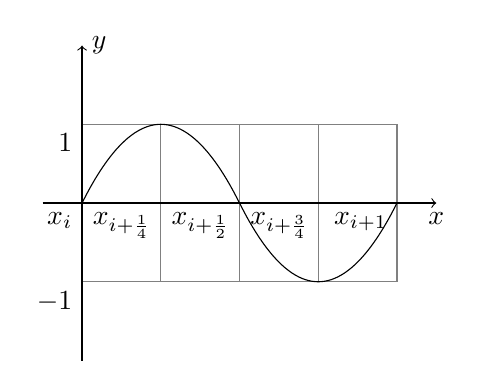
\begin{tikzpicture}[scale = 1]
	\draw[gray, step = 1cm] (0, -1) grid (4, 1);
	\draw[->] (-.5, 0) -- (4.5, 0);
	\draw[->] (0, -2) -- (0, 2);
	
	\node[anchor = north east] at (0, 0) {$ x_i $};
	\node[anchor = north east] at (1, 0) {$ x_{i+\frac{1}{4}} $};
	\node[anchor = north east] at (2, 0) {$ x_{i+\frac{1}{2}} $};
	\node[anchor = north east] at (3, 0) {$ x_{i+\frac{3}{4}} $};
	\node[anchor = north east] at (4, 0) {$ x_{i+1} $};
	\node[anchor = north east] at (0, 1) {$ 1 $};
	\node[anchor = north east] at (0, -1) {$ -1 $};
	\node[anchor = north] at (4.5, 0) {$ x $};
	\node[anchor = west] at (0, 2) {$ y $};
	
	
	\draw[domain = 0:2, smooth, variable=\x, black]
	plot ({\x}, {\x * (2-\x)})
	node[anchor = west] {};
	\draw[domain = 2:4, smooth, variable=\x, black]
	plot ({\x}, {-(4-\x) * (\x-2)})
	node[anchor = west] {};
	\end{tikzpicture}
\end{center}

We sum all the function on $[0,1]$,
\[
(I_{k+1}-I_k)(x^3) = 3\times2^{-3k-6}\sum_{i=0}^{2^k-1}(\varphi_{i+\frac{1}{4}}^{k+1} - \varphi_{i+\frac{3}{4}}^{k+1})
\]


\section{2D sparse grid for $xy$}
Consider the uniform gird $[0,1]^2$, and we define the grid
\[
T_k:(x_i,y_j),\quad x_i = ih,y_j = jh,\quad h = 2^{-k}
\]
$I_k$ is the piece linear interpolation operator which satisfies 
\[
(I_k f)(x_i,y_j) = f(x_i,y_j)
\]
We consider the grid $T_k$ and $T_{k-1}$. 
\begin{itemize}
	\item The basis functions on $T_{k-1}$ are $\varphi_1^{k-1},\varphi_2^{k-1},\varphi_3^{k-1}$.
	\item  The basis functions on refine grid $T_k$ are $\varphi_i^k,i=1,..,6$.
\end{itemize}
\begin{center}
	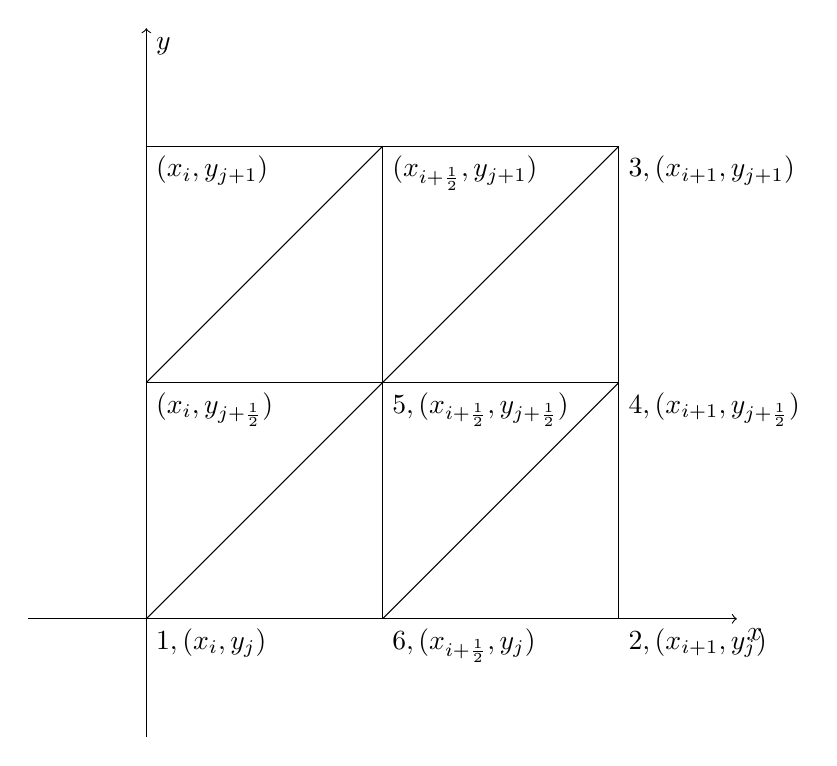
\begin{tikzpicture}[scale = 3 ]
	\draw[gray, step = 1cm] (0, 0) grid (2, 2);
	\draw[->] (-.5, 0) -- (2.5, 0);
	\draw[->] (0, -.5) -- (0, 2.5);
	\node[anchor = north west] at (0, 0) {$1, (x_i,y_j) $};
	\node[anchor = north west] at (2.5, 0) {$ x $};
	\node[anchor = north west] at (0, 2.5) {$ y $};
	\node[anchor = north west] at (1,0) {$6,(x_{i+\frac{1}{2}},y_j)$};
	\node[anchor = north west] at (2,0) {$2,(x_{i+1},y_j)$};
	\node[anchor = north west] at (0,1) {$(x_{i},y_{j+\frac{1}{2}})$};
	\node[anchor = north west] at (1,1) {$5,(x_{i+\frac{1}{2}},y_{j+\frac{1}{2}})$};
	\node[anchor = north west] at (2,1) {$4,(x_{i+1},y_{j+\frac{1}{2}})$};
	\node[anchor = north west] at (0,2) {$(x_{i},y_{j+1})$};
	\node[anchor = north west] at (1,2) {$(x_{i+\frac{1}{2}},y_{j+1})$};
	\node[anchor = north west] at (2,2) {$3,(x_{i+1},y_{j+1})$};
	
	\draw (0,0) -- (0,2);
	\draw (0,2) -- (2,2);
	\draw (2,2) -- (2,0);
	\draw (2,0) -- (0,0);
	\draw (0,0) -- (2,2);
	\draw (0,1) -- (1,2);
	\draw (1,0) -- (2,1);
	\draw (1,0) -- (1,2);
	\draw (0,1) -- (2,1);
	\end{tikzpicture}
\end{center}
\[
\begin{split}
I_{k-1}(xy) &= x_iy_j\varphi^{k-1}_1 + x_{i+1}y_j\varphi^{k-1}_2 + x_{i+1}y_{j+1}\varphi^{k-1}_3\\
&=x_iy_j(\varphi^k_1 + \frac{1}{2}(\varphi^k_5+\varphi^k_6)) + x_{i+1}y_j(\varphi^k_2 + \frac{1}{2}(\varphi^k_4+\varphi^k_6))\\
&+x_{i+1}y_{j+1}(\varphi^k_3+\frac{1}{2}(\varphi^k_4+\varphi^k_5))\\
&=x_iy_j\varphi^k_1 + x_{i+1}y_j\varphi^k_2+x_{i+1}y_{j+1}\varphi^k_3+\frac{1}{2}(x_{i+1}y_j+x_{i+1}y_{j+1})\varphi^k_4\\
&+\frac{1}{2}(x_{i}y_j+x_{i+1}y_{j+1})\varphi^k_5+\frac{1}{2}(x_{i}y_j+x_{i+1}y_{i})\varphi^k_6\\
&=x_iy_j\varphi^k_1 + x_{i+1}y_j\varphi^k_2+x_{i+1}y_{j+1}\varphi^k_3+x_{i+1}y_{j+\frac{1}{2}}\varphi^k_4\\
&+\frac{1}{2}(x_{i}y_j+x_{i+1}y_{j+1})\varphi^k_5+x_{i+\frac{1}{2}}y_j\varphi^k_6\\
I_k(xy) & = x_iy_j\varphi^k_1+x_{i+1}y_j\varphi^k_2+x_{i+1}y_{j+1}\varphi^k_3+x_{i+1}y_{j+\frac{1}{2}}\varphi^k_4 \\
&+x_{i+\frac{1}{2}}y_{j+\frac{1}{2}}\varphi^k_5 + x_{i+\frac{1}{2}}y_j\varphi^k_6
\end{split}
\]

Then,
\[
(I_k - I_{k-1})(xy) = (x_{i+\frac{1}{2}}y_{j+\frac{1}{2}}-\frac{1}{2}(x_{i}y_j+x_{i+1}y_{j+1}))\varphi^k_5 = -\frac{h^2}{4}\varphi_5^k
\]
The error is uniform! which is the basis function on each rectangle $[x_i,x_{i+1}]\times [y_j,y_{j+1}]$ and 
\[
\varphi_5^k(x_{i+\frac{1}{2}},y_{j+\frac{1}{2}}) = 1
\]


\section{Spectral approximation properties of ReLU DNN}
Here we will talk about how to use ReLU DNN to approximate polynomials
and then achieve the ``spectral" accuracy for analytical functions.
The main results can be found in \cite{yarotsky2017error},
\cite{wang2018exponential}. Some related works are
\cite{liang2016why,lu2017expressive}

First, we will introduce the following notation
\begin{itemize}
\item $x=(x_1,\ldots,x_d)$.
\item Colon notation for subscript: let $\{x_{m:n}\} = \{x_i:i = m,m+1,...,n\}$ and $\{x_{m_1:n_1,m_2:n_2}\}= \{x_{i,j}:i = m_1,...,n_1,j = m_2,...,n_2\}.$ 
\item Linear combination: denote $y\in \mathcal L(x_1,...,x_d)$ if
  there exist $\beta_i\in \mathbb{R},i=1,...,d,$ such that $y =
  \beta_0+\beta_1x_1+\cdots+\beta_d x_d$.
\item Linear combination with ReLU activation: denote $\tilde{y}\in
  \tilde{\mathcal L}(x_1,...,x_d)$ if there exists $y\in
  \mathcal{L}(x_1,...,x_d)$ and $\tilde{y} = \mbox{ReLU}(y) =
  \max(y,0).$
\item $\tilde {\mathcal L} =\sigma\circ\mathcal L$
\end{itemize}
\begin{definition}
Given a function $f(x)$, if there exist variables $\{y_{1:L,1:M}\}$ such that 
\begin{equation}
y_{1,m}\in \tilde{\mathcal L}(x),\quad y_{l+1,m} \in \tilde{\mathcal L}(x,y_{l,1:M}),\quad f\in\mathcal{L}(x,y_{1:L,1:M}),
\end{equation}\label{def:netclass}
where $m=1,...,M,l=1,...,L-1$, then $f$ is said to be in the neural nets class $\mathcal{F}_{L,M}(\mathbb{R}^d)$, and $\{y_{1:L,1:M}\}$ is called a set of hidden variables of $f$. 
\end{definition}
\newpage
%\begin{properties}
\begin{proposition}
A function $f\in \mathcal F_{L,M}(\mathbb R^d)$ can be represented by a ReLU network with depth $L+1$ and width $M+d+1$.
\end{proposition}
%\end{properties}
\begin{proof}
Let $\{y_{1:L}\}$ be the hidden variables of $f$ that satisfies (\ref{def:netclass}), where
$$
f = \alpha_0 + \sum_{i=1}^d \alpha_ix_i+\sum_{l=1}^L\sum_{m=1}^M \beta_{l,m}y_{l,m}.
$$
$$
h\leftarrow (y,ex^T), e=(1,\ldots 1)^T.
$$
Consider the following variables $\{h_{1:L,1:M}\}$:
$$
h_{l,1:M} = y_{l,1:M}, \quad h_{l,M+1:M+d} = x_{1:d}
$$
for $l = 1,...,L,$ and
$$
h_{1,M+d+1} = \alpha_0 + \sum_{i=1}^d\alpha_ix_i,\quad h_{l+1,M+d+1} =h_{l,M+d+1} + \sum_{m=1}^M\beta_{l,m}h_{l,m}
$$
for $l=1,...,L-1$. One can see that $h_{1,m}\in \tilde{\mathcal L}(x),h_{l+1,m}\in \tilde{L}(h_{l,1:M+d+1}),m = 1,...,M+d+1,l = 1,...,L-1,$ and $f\in \mathcal{L}(h_{L,1:M+d+1}),$ which is a representation of a standard neural net.
\end{proof}

%\begin{properties}
\begin{proposition}\label{prop:net class}
(Addition and composition of neural net class $\mathcal F_{L,M}$)
\begin{itemize}
\item[1]
$$
\mathcal F_{L_1,M} + \mathcal{F}_{L_2,M} \subseteq \mathcal{F}_{L_1+L_2,M},
$$
i.e. if $f_1\in \mathcal F_{L_1,M}(\mathbb{R}^d)$ and $f_2\in \mathcal{F}_{L_2,M}(\mathbb{R}^d),$ then $f_1+f_2\in\mathcal{F}_{L_1+L_2,M}(\mathbb{R}^d)$.
\item[2]
$$
\mathcal F_{L_2,M}\circ \mathcal F_{L_1,M+1} \subseteq \mathcal F_{L_1+L_2,M+1}.
$$ 
i.e. if $f_1(x)\in \mathcal{F}_{L_1,M+1}(\mathbb{R}^d)$ and $f_2(x_0,x)\in \mathcal{F}_{L_2,M}(\mathbb{R}^{d+1}),$ then 
$$
f_2(f_1(x),x)\in \mathcal{F}_{L_1+L_2,M+1}(\mathbb{R}^d).
$$
\end{itemize}
\end{proposition}
%\end{properties}

\newpage
\begin{proof}
For the addition property, denote the hidden variables of $f_1$ and $f_2$ as $\{y_{1:L_1,1:M}^{(1)}\}$ and $\{y_{1:L_2,1:M}^{(2)}\}$. 
So we have 
\[
f_1 = \alpha_0^1 + \sum_{i=1}^d \alpha^1_ix_i+\sum_{l=1}^L\sum_{m=1}^M \beta^1_{l,m}y^{(1)}_{l,m}
\]
\[
f_2 = \alpha_0^2 + \sum_{i=1}^d \alpha^2_ix_i+\sum_{l=1}^L\sum_{m=1}^M \beta^2_{l,m}y^{(2)}_{l,m}
\]
\[
f_1+f_2 = \alpha_0^1 + \alpha_0^2 + \sum_{i=1}^d (\alpha_i^1+\alpha_i^2)x_i + \sum_{l=1}^L\sum_{m=1}^M \beta^1_{l,m}y^{(1)}_{l,m} +\sum_{l=1}^L\sum_{m=1}^M \beta^2_{l,m}y^{(2)}_{l,m}
\]
$$
y^{(1)}_{1,1:M} = \sigma\circ \mathcal{L}(x),y^{(1)}_{2,1:M} = \sigma\circ \mathcal L(x,y^{(1)}_{1,1:M}),\cdots,y^{(1)}_{L_1,1:M}=\sigma\circ \mathcal L(x,y^{(1)}_{L_1-1,1:M}),
$$
$$
y^{(2)}_{1,1:M} = \sigma\circ \mathcal{L}(x) =\sigma(\mathcal L(x)+\bm 0\cdot y^{(1)}_{L_1,1:M}) = \sigma\circ \mathcal{L}(x,y^{(1)}_{L_1,1:M})
$$
$$
y^{(2)}_{2,1:M} = \sigma\circ \mathcal L(x,y^{(2)}_{1,1:M}),\cdots,y^{(2)}_{L_2,1:M}=\sigma\circ \mathcal L(x,y^{(2)}_{L_2-1,1:M}),
$$
so $f_1 + f_2 \in \mathcal{F}_{L_1+L_2,M}$
Let
$$
y_{1:L_1,1:M} = y_{1:L_1,1:M}^{(1)},\quad y_{L_1+1:L_1+L_2,1:M} = y_{1:L_2,1:M}^{(2)}. 
$$
By definition, $\{y_{1:L_1+L_2,1:M}\}$ is a set of hidden variables of $f_1+f_2$. Thus $f_1+f_2\in \mathcal F_{L_1+L_2,M}.$

For the composition property, let the hidden variables of $f_1$ and $f_1$ as $\{y_{1:L_1,1:M+1}^{(1)}\}$ and $\{y_{1:L_2,1:M}^{(2)}\}$. Let
$$
y_{1:L_1,1:M+1} = y_{1:L_1,1:M+1}^{(1)},\quad y_{L_1+1:L_1+L_2,1:M} = y_{1:L_2,1:M}^{(2)},
$$
$$
y_{L_1+1,M+1} =\cdots= y_{L_1+L_2,M+1} = f_1(x).
$$
One can see that $\{y_{1:L_1+L_2,1:M+1}\}$ is a set of hidden variables of $f_2(f_1(\bm x),\bm x)$, thus the composition property holds.
\end{proof}

\begin{definition}
Given a continuous function $\varphi(\bm{x}),\bm{x} \in [-1,1]^d$ and a continuous function class $\mathcal F([-1,1]^d),$ define the $L^\infty$ distance
$$
\mbox{dist} (\varphi,\mathcal F) = \inf_{f\in \mathcal F} \max_{\bm x \in [-1,1]^d} |\varphi(\bm{x}) - f(\bm{x})|.
$$
\end{definition}

%\begin{properties}
\begin{proposition}\label{prop:dis}
(Addition and composition properties for distance function)
\begin{itemize}
\item[1] Let $\varphi_1$ and $\varphi_2$ be continuous functions. Let $\mathcal F_{1}$ and $\mathcal F_2$ be two continuous function classes, then 
$$
\mbox{dist}(\alpha_{1}\varphi_1+\alpha_{2}\varphi_2,\mathcal{F}_1+\mathcal F_2)\le |\alpha_1|\mbox{dist}(\varphi_1,\mathcal F_1) + |\alpha_2|\mbox{dist}(\varphi_2,\mathcal F_2),
$$
where $\alpha_1$ and $\alpha_2$ are two real numbers.
\item[2] Assume that $\varphi_1(\bm x) = \varphi_1(x_1,...,x_d),\varphi_2(y,\bm x) = \varphi_2(y,x_1,...,x_d)$ satisfy $\varphi_1([-1,1]^d)\subseteq[-1,1]$. Let $\mathcal F_1([-1,1]^d),\mathcal F_2([-1,1]^{d+1})$ be two continuous function classes, then
$$
\mbox{dist}(\varphi_2(\varphi_1(\bm x),\bm x),\mathcal F_2\circ \mathcal F_1)\le L_{\varphi_2}\mbox{dist}(\varphi_1,\mathcal F_1) +\mbox{dist}(\varphi_2,\mathcal F_2)
$$
where $L_{\varphi_2}$ is the Lipschitz norm of $\varphi_2$ with respect to $y$.
\end{itemize}
\end{proposition}
%\end{properties}
\begin{proof}
The additional property obviously holds. Now we prove the composition property. For any $f_1\in\mathcal F_1,f_2\in \mathcal F_2$, one has
\[
\begin{split}
|\varphi_2(\varphi_1(\bm x),\bm x) - f_2(f_1(\bm x),\bm x)|&\le |\varphi_2(\varphi_1(\bm x),\bm x) - \varphi_2(f_1(\bm x),\bm x)|+|\varphi_2(f_1(\bm x),\bm x)-f_2(f_1(\bm x),\bm x)|\\
& \le L_{\varphi_2} ||\varphi_1(\bm x) -f_1(\bm x)||_\infty +||\varphi_2(y,\bm x) - f_2(y,\bm x)||_\infty
\end{split}
\]
Take $f_1^* = \argmin_f ||\varphi_1(\bm x) - f(\bm x)||_\infty$ and $f_2^* = \argmin_f ||\varphi_2(y,\bm x) - f(y,\bm x)||_\infty$, then it is proved.
\end{proof}

\begin{lemma}\label{lem:xsquare}
The function $\varphi(x) = x^2,x\in [-1,1]$ can be approximated by deep neural nets with an exponential convergence rate:
$$
\mbox{dist}(x^2,\mathcal{F}_{L,2}([-1,1]))\le 2^{-2L}.
$$
\end{lemma}
\begin{proof}
Consider the function
$$
g(y) = \left\{\begin{split}
	&2y,&\quad 0\le y<1/2,\\
	&2(1-y),&\quad 1/2\le y\le 1,
	\end{split}\right.
$$
then 
\begin{equation}\label{func:g}
g(y) = 2y -4\mbox{ReLU}(y-1/2)
\end{equation}
in $[0,1]$. Define the hidden variables $\{y_{1:L,1:2}\}$ as follows:
\[
\begin{split}
 y_{1,1} = \mbox{ReLU}(x),&\quad y_{1,2}=\mbox{ReLU}(-x),\\
 y_{2,1} = \mbox{ReLU}(y_{1,1}+y_{1,2}),&\quad y_{2,2} = \mbox{ReLU}(y_{1,1}+y_{1,2}-1/2),\\
 y_{2,1} = \mbox{ReLU}(|x|),&\quad y_{2,2} = \mbox{ReLU}(|x|-1/2),\\
 y_{l+1,1} = \mbox{ReLU}(2y_{l,1}-4y_{l,2}),&\quad y_{l+1,2} = \mbox{ReLU}(2y_{l,1}-4y_{l,2}-1/2)\\
\end{split}
\]
for $l = 2,3,...,L-1$. Using induction, one can see that $|x| = y_{1,1}+y_{1,2}$ and 
\begin{equation}\label{func:glinduction}
g_l(|x|)=\underbrace{g\circ g\circ \cdots \circ g}_{l}(|x|) = 2y_{l+1,1}-4y_{l+1,2},\quad l=1,...,L-1,
\end{equation} 
for $x\in [-1,1]$. i.e.
\[
\begin{split}
g_l(|x|) &= g\left(g_{l-1}(|x|)\right)\\
         &= g(2y_{l,1}-4y_{l,2})\qquad (\mbox{Eq~(\ref{func:g})})\\
         &= 2(2y_{l,1}-4y_{l,2}) - 4\mbox{ReLU}(2y_{l,1}-4y_{l,2}-1/2)\qquad (g_{l-1}(|x|)\ge 0~\mbox{if}~x\in[0,1])\\
         &= 2\mbox{ReLU}(2y_{l,1}-4y_{l,2})- 4\mbox{ReLU}(2y_{l,1}-4y_{l,2}-1/2)\\
         & = 2y_{l+1,1} - 4y_{l+1,2}\\
\end{split}
\]
by induction, Eq (\ref{func:glinduction}) holds.
\begin{figure}[h]
	\centering
	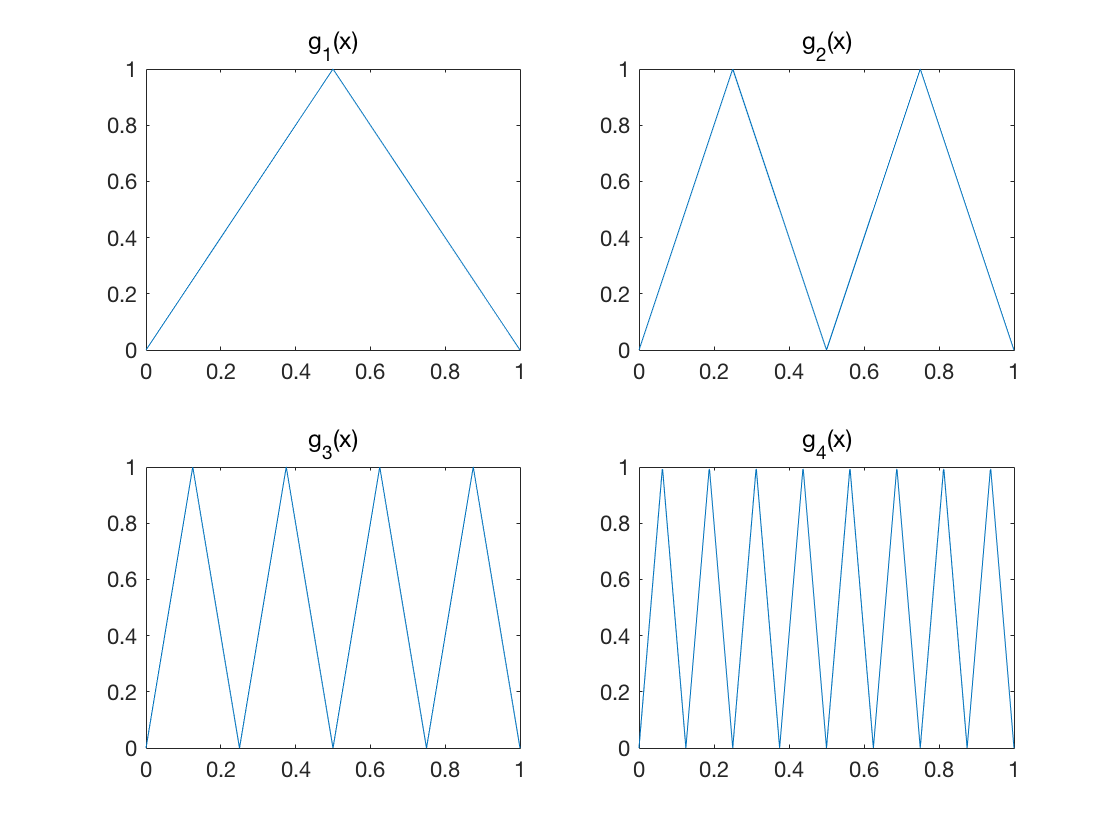
\includegraphics[width=0.8\textwidth]{figures/dl_approx_analytic_gl}
	\caption{The figure of $g_l(x)$}
	\label{fig:gl}
\end{figure}

Let $f_m$ be the piecewise linear interpolation of $f$ with $2^m+1$ uniformly distributed breakpoints $\frac{k}{2^m},k = 0,...,2^m:$
$$
f_{m}(\frac{k}{2^m}) = (\frac{k}{2^m})^2,\quad k = 0,...,2^m.
$$
Note that refining the interpolation from $f_{m-1}$ to $f_m$ amounts to adjusting it by a function proportional to a sawtooth function:
$$
f_{m-1}(x) - f_m(x) = \frac{g_m(x)}{2^{2m}}.
$$
Hence 
$$
f_{L-1}(|x|) = |x| - \sum_{l=1}^{L-1}\frac{g_l(|x|)}{2^{2l}} .
$$
then $f_{L-1}\in \mathcal{F}_{L,2}$, and 
\[
\begin{split}
||x^2-f_{L-1}(x)||_{\infty} & = \max_{k} \max_{x\in [\frac{k}{2^{L-1}},\frac{k+1}{2^{L-1}}]} |x^2 - f_{L-1}(x)|\\
  & = \max_{k} |(\frac{1}{2}(\frac{k}{2^{L-1}}+\frac{k+1}{2^{L-1}}))^2 - f_{L-1}(\frac{1}{2}(\frac{k}{2^{L-1}}+\frac{k+1}{2^{L-1}}))|\\
  & = \max_k |(\frac{1}{2}(\frac{k}{2^{L-1}}+\frac{k+1}{2^{L-1}}))^2 - \frac{1}{2}((\frac{k}{2^{L-1}})^2+(\frac{k+1}{2^{L-1}})^2))|\\
  &=\frac{1}{4^L}.
\end{split}
\]
$|x^2-f_{L-1}(x)|\le 2^{-2L}$ for $x\in[-1,1].$
\end{proof}

\begin{lemma}\label{lem:xy}
For multiplication function $\varphi(x,y) = xy$, we have 
$$
\mbox{dist}(xy,\mathcal{F}_{3L,2}([-1,1]^2))\le 3\cdot 2^{-2L}.
$$
\begin{proof}
Notice that
$$
\varphi = xy = 2\left(\frac{x+y}{2} \right)^2-\frac{1}{2}x^2-\frac{1}{2}y^2.
$$
\[
\begin{split}
\mbox{dist}(xy,\mathcal{F}_{3L,2}([-1,1]^d))&\le2\mbox{dist}(\left(\frac{x+y}{2} \right)^2,\mathcal{F}_{L,2}([-1,1]^2)) + \frac{1}{2} \mbox{dist}(x^2,\mathcal{F}_{L,2}([-1,1]^2)) \\
 &+\frac{1}{2} \mbox{dist}(y^2,\mathcal{F}_{L,2}([-1,1]^2))\\
 &\le 3\mbox{dist}(x^2,\mathcal{F}_{L,2}([-1,1]^2))\\
 &\le 3\mbox{dist}(x^2,\mathcal{F}_{L,2}([-1,1])) + \mbox{dist}(I_x,\mathcal{F}_{L,2}([-1,1]^2))\\
 &= 3\cdot 2^{-2L}
\end{split}
\]
\end{proof}
\end{lemma}

\begin{lemma}
For a monomial $M_p(\bm x)$ of $d$ variables with degree $p$, we have
$$
\mbox{dist}(M_p,\mathcal F_{3(p-1)L,3}(\mathbb R^d))\le 3(p-1)\cdot 2^{-2L}.
$$
\end{lemma}

\begin{proof}
Let $M_p(\bm x)=x_{i_1}x_{i_2}\cdots x_{i_p},i_1,...,i_p\in\{1,...,d\}.$ Using induction, assume that the lemma holds for the degree-$p$ monomial $M_p$, consider a degree-$(p+1)$ monomial $M_{p+1}(\bm{x}) = M_p(\bm{x})\cdot x_{i_{p+1}}$. Let $\varphi(y,x) = yx,$ then $M_{p+1}(\bm x) = \varphi(M_p(\bm{x}),x_{i_{p+1}})$. We have
\[
\begin{split}
\mbox{dist}(M_{p+1},\mathcal{F}_{3pL,3})&\le \mbox{dist}(\varphi(M_p(\bm x),x_{i_{p+1}}),\mathcal F_{3L,2}\circ \mathcal F_{3(p-1)L,3})\\
& \le L_{\varphi}\mbox{dist}(M_p,\mathcal{F}_{3(p-1)L,3})+\mbox{dist}(\varphi,\mathcal F_{3L,2})\le 3p\cdot 2^{-2L}.
\end{split}
\]
Note that the Lipschitz norm $L_{\varphi}=1$ since $x_{i_{p+1}}\in [-1,1].$
\end{proof}

\begin{lemma}
For a degree-$p$ polynomial $P_p(\bm{x}) = \sum_{|\bm{k}|\le p}a_{\bm k}\bm x^{\bm k},\bm x\in [-1,1]^d,\bm k = (k_1,...,k_d)\in\mathbb{N}^d,$ we have 
\[
\mbox{dist}\left(P_p,\mathcal F_{\binom{p+d}{d}(p-1)L,3}\right)<3(p-1)\cdot 2^{-2L}\sum_{|\bm k|\le p}|a_{\bm k}|
\]
\end{lemma}\label{lem:poly}

\begin{proof}
This lemma can be proved by the properties \ref{prop:net class}, \ref{prop:dis} and lemma \ref{lem:poly}.
Note that the number of monomials of $d$ variables with degree less or equal to $p$ is $\binom{p+d}{d}$.
$$
k_1 + k_2 + \cdots + k_d \le p,
$$
Add a variable $k_{d+1}$, we have
$$
k_1 + k_2 + \cdots + k_d + k_{d+1} = p.
$$
the number of the non-negative solution is $\binom{p+d}{d}$.
\end{proof}

\begin{theorem}
Let $f$ be an analytic function over $(-1,1)^d$. Assume that the power series $f(\bm x) = \sum_{\bm k\in \mathbb N^d}a_{\bm k}\bm x^{\bm k}$ is absolutely convergent in $[-1,1]^d.$ Then for any $\delta>0,$ there exists a function $\hat f$ that can be represented by a deep ReLU network with depth $L$ and width $d+4$, such that
\[
|f(\bm x) - \hat f(\bm x)|<2\sum_{\bm k\in \mathbb N^d}|a_{\bm k}|\cdot \exp\left(-d\delta\left(e^{-1}L^{1/2d}-1\right)\right)
\]
for all $\bm x\in [-1+\delta,1-\delta]^d.$
\end{theorem}
\begin{proof}
Let $\epsilon = \exp(-d\delta(e^{-1}L^{1/2d}-1)),$ then $L = [e(\frac{1}{d\delta}\log\frac{1}{\epsilon}+1)]^{2d}$. Without loss of generality, assume $\sum_{\bm k}|a_{\bm k}|=1.$ We will show that there exists $\hat f\in \mathcal F_{L,3}$ such that $||f-\hat f||_{\infty}<2\epsilon.$
Denote 
$$
f(\bm x) = P_p(\bm x) + R(\bm x): = \sum_{|\bm k|\le p}a_{\bm k}\bm x^{\bm k} +  \sum_{|\bm k|> p}a_{\bm k}\bm x^{\bm k}.
$$
For $\bm x\in [-1+\delta,1-\delta]^d$, we have $|R(\bm x)|<(1-\delta)^p$, thus truncation to $p = \frac{1}{\delta}\log\frac{1}{\epsilon}$ with ensure $|R(\bm x)|<2\epsilon$. From lemma \ref{lem:poly}, we have dist$(P_p,\mathcal F_{L,3})<3(p-1)\cdot 2^{-2L'}$, where 
\[
\begin{split}
L' &= L\binom{p+d}{d}^{-1}(p-1)^{-1}\\
   &\ge L(\frac{(p+d)!}{p!d!})^{-1}p^{-1}\quad (d! \thicksim \sqrt{2\pi d}(d/e)^d)\\
   &\ge L(\frac{(p+d)^d}{(d/e)^d})^{-1}p^{-1}\\
   &= L[e(\frac{1}{d\delta}\log \frac{1}{\epsilon}+1)]^{-d}(\frac{1}{\delta}\log\frac{1}{\epsilon})^{-1}\\
   & = [e(\frac{1}{d\delta}\log \frac{1}{\epsilon}+1)]^{d}(\frac{1}{\delta}\log\frac{1}{\epsilon})^{-1}\\
   & \ge e^d (\frac{1}{\delta}\log\frac{1}{\epsilon}) \\
   &\gg\log\frac{1}{\delta}+ \log\frac{1}{\epsilon}
\end{split}
\]
for $d\ge 2$ and $\epsilon\ll 1$, then dist$(P_p,\mathcal F_{L,3})<3(p-1)\cdot 2^{-2L'} = 3(p-1)(\epsilon^2+\delta^2)\ll\epsilon$. Thus there exists $\hat f\in \mathcal F_{L,3}$ such that $||P_p - \hat f||_{\infty}<\epsilon$, and $||f-\hat f||_{\infty}\le ||f-P_p||_\infty + ||P_p - \hat f||_\infty<3\epsilon$.
\end{proof}

\subsection{Cosine Function}

Let $f(\bm x) = \cos(|\bm x|^2)$. Assume that the power series 
\[
f(\bm x) = \sum_{k=0}^{+\infty} \frac{(-1)^k|\bm x|^{4k}}{(2k)!},\quad \bm x\in [-1,1]^d.
\]
Denote
\[
\begin{split}
f(\bm x) = P_p(\bm x) + R(\bm x): &= \sum_{|\bm k|\le p}a_{\bm k} \bm x^{\bm k} + \sum_{|\bm k|>p} a_{\bm k} \bm x^{\bm k}\\
&=\sum_{k\le p} \frac{(-1)^k}{(2k)!}|\bm x|^{4 k} + \frac{(-1)^{p+1}}{(2(p+1))!}|\bm t|^{4 (p+1)},\quad \bm t\in[0,1]^d\\
\end{split}
\]


Let $p(\varepsilon,d)=p$ be large, s.t.
\[
\big|\frac{(-1)^{p+1}}{(2(p+1))!}|\bm t|^{4(p+1)}\big| < \varepsilon.
\]
\[
\begin{split}
\big|\frac{(-1)^{p+1}}{(2(p+1))!}|\bm t|^{4 (p+1)}\big| &\le \frac{d^{2(p+1)}}{(2(p+1))!}\\
& \le C(\frac{ed}{2(p+1)})^{2(p+1)}\\
\end{split}
\]
Let $p = \log \frac{1}{\varepsilon}-1$, then 
\[
(\frac{ed}{2(p+1)})^{2(p+1)}\le (\frac{ed}{2\log \frac{1}{\varepsilon}})^{2\log\frac{1}{\varepsilon}}\le \varepsilon^{-2\log \frac{ed}{2\log \frac{1}{\varepsilon}}}\le \varepsilon
\]

We want to show that 
\[
\mbox{dist}(P_{p(\varepsilon,d)},\mathcal{F}_{L(\varepsilon,d),3})<\varepsilon.
\]

By Lemma~\ref{lem:poly}, we have 
\[
\begin{split}
\mbox{dist}(P_{p},\mathcal{F}_{L,3})&<3(p-1)2^{-\frac{2L}{\binom{p+d}{d}(p-1)}}\sum_{\bm k\le p}|a_{\bm k}|\\
&\le3p2^{-\frac{2Ld^d}{p(p+d)^de^d}}\sum_{|\bm k|\le p}|a_{\bm k}|.
\end{split}
\]

Let $L = \frac{1}{2} ((p+d)e/d)^{2d}$, we can see that
\[
\begin{split}
\mbox{dist}(P_{p},\mathcal{F}_{L,3})
&\le3p2^{-\frac{2Ld^d}{p(p+d)^de^d}}\sum_{|\bm k|\le p}|a_{\bm k}|\\
&= 3p2^{-\frac{(p+d)^de^d}{d^dp}}\sum_{|\bm k|\le p}|a_{\bm k}|\\
&\le 3(\log \frac{1}{\varepsilon}-1)2^{-\frac{e^d}{4}(d-1)d(\log \frac{1}{\varepsilon}-1)} \sum_{|\bm k|\le p}|a_{\bm k}|\\
&\le C(d)\varepsilon^{\frac{e^d}{4}d(d-1)\log 2}\log\frac{1}{\varepsilon}\le \varepsilon
\end{split}
\]

Take 
\[
\varepsilon = \exp\left(-d\left(e^{-1}(2L)^{1/2d}-1\right)-1\right)
\]
then, we have 
\[
\mbox{dist}(f,\mathcal{F}_{L,3})\le\mbox{dist}(P_{p},\mathcal{F}_{L,3})+ R(\bm x) \le 2\varepsilon \le 2e^{-d\left(e^{-1}(2L)^{1/2d}-1\right)-1}
\]



\section{A modified ResNet structure and its properties}
Using the notation in Lin Li's notes, we have the next two properties for this modified ResNet structure in $\mathbb{R}^d$ as
\begin{itemize}
	\item Added with depth
	$$
	\mathcal F_{L_1,M}(\mathbb{R}^d) + \mathcal{F}_{L_2,M}(\mathbb{R}^d)  \subseteq \mathcal{F}_{L_1+L_2,M}(\mathbb{R}^d) .
	$$
	\item Added with width 
	$$
	\mathcal F_{L,M_1}(\mathbb{R}^d)  + \mathcal{F}_{L,M_2}(\mathbb{R}^d)  \subseteq \mathcal{F}_{L,M_1 + M_2}(\mathbb{R}^d) .
	$$
\end{itemize}
This second property works for all DNN structures, but the first structure only works for this special ResNet structure with any activation functions.

\section{h-method by partition of unit}
First, for any positive integer $M$, let us consider the next partition of unit function of $[0, 1]^d$
$$
\phi_{\bm m}(x) = \prod_{k=1}^d \Phi\left(3M(x_k - \frac{m_k}{M})\right),
$$
with 
$$
{\bm m} = (m_1, m_2, \cdots, m_d) \in \{0,1, \cdots,M\}^d = \mathcal{M},
$$
and 
$$
\Phi(x) = \begin{cases}
1, \quad  &|x| \le 1, \\
0, \quad &|x| \ge 2, \\
2 - |x|, \quad &1 < |x| <2.
\end{cases}
$$
Thus, we have
$$
\sum_{{\bm m} \in \mathcal{M}} \phi_{\bm m}({\bm x}) = 1, \quad \forall {\bm x} \in [0,1]^d.
$$

\begin{itemize}
	\item How to choose M?
\end{itemize}
\section{p-method by local Taylor expansion}
Taylor expansion with $p-$th polynomials at most at ${\bm x} = \frac{{\bm m}}{M}$:
$$
P_{{\bm m}, p}({\bm x}) = \sum_{|{\bm n}| < p}\frac{\partial^{\bm n}f}{ \bm n !}\left(\frac{{\bm m}}{M}\right) ({\bm x} - \frac{{\bm m}}{M})^{\bm n}.
$$
Here we just consider about the local Taylor expansion, so the global approximation function is
$$
f_p({\bm x}) = \sum_{{\bm m} \in \mathcal{M}} \phi_{\bm m} P_{{\bm m}, p}({\bm x}), \quad \forall {\bm x} \in [0,1]^d.
$$

\begin{itemize}
	\item How to choose $p$? Balance with the residual term?
\end{itemize}

\section{Error estimate for $|f - f_p|_{0,\infty}$}
\begin{align*}\label{fperoor}
|f - f_p|_{0,\infty} &= |\sum_{\bm m} \phi_{\bm m}(f - P_{{\bm m}, p})|_{0, \infty},  \\
&\le \max_{{\bm m} \in \mathcal{M}}  |\sum_{\bm m} \phi_{\bm m}(f - P_{{\bm m}, p})|_{0, \infty,  |{\bm x} - \frac{\bm m}{M}| \le {\frac{1}{M}}}, \\
&\le \max_{{\bm m} \in \mathcal{M}} \sum_{ {\bm m} \in \mathcal{N}({\bm m})} |f - P_{{\bm m}, p}|_{0,\infty, |{\bm x} - \frac{\bm m}{M}| \le {\frac{1}{M}}}, \\
&\le \max_{{\bm m} \in \mathcal{M}}  2^d \max_{{\bm m} \in \mathcal{N}({\bm m})} |f - P_{{\bm m}, p}|_{0,\infty, |{\bm x} - \frac{\bm m}{M}| \le {\frac{1}{M}}}, \\
&\le \left( 2^{d} \left( \frac{1}{M} \right)^p \frac{d^p}{ p!} \right)|f|_{p, \infty}.
\end{align*}

\section{Approximate $f_p$ by ReLU DNN with error estimate}
\subsection{Approximate $\phi_m P_{m, p}$}
\begin{itemize}
	\item Approximate $\phi_{\bm m}$ 
	
	First we know that 
	$$
	\Phi(x) = ReLU(x+2) - ReLU(x+1) - ReLU(x-1) + ReLU(x-2),
	$$ 
	so 
	$$
	\inf_{v \in DNN_{J}} |\phi_{\bm m} - v| \le 2^{-\frac{2J}{3d}}.
	$$
	\item Approximate $P_{{\bm m}, p}$ (Original version in Yarotsky2017 )
	
	Assume that 
	$$
	P_{{\bm m}, p} = \sum_{|{\bm n}| \le p}a_{\bm m, \bm n} {(\bm x - \frac{\bm m}{M})}^{\bm n},
	$$
	then 
	$$
	\inf_{v \in DNN^{T}_{J}} |P_{{\bm m}, p} - v| \le (\max_{ \bm n} a_{\bm m,\bm n})2^{-\frac{2J}{3(p-1)}},
	$$
	with 
	$$
	T = \tbinom{p+d}{d}(d+4).
	$$
	
	\item Approximate $\phi_{\bm m} P_{\bm m, p}$
	$$
	\inf_{v \in DNN^{T}_{J}} |\phi_{\bm m} P_{\bm m, p} - v| \le (\max_{ \bm n} a_{\bm m,\bm n}) \max\{2^{-\frac{2J}{9(p-1)}},  2^{-\frac{2J}{9d}}\},
	$$
\end{itemize}

\begin{remark}
In fact, in Yarotsky2017 they estimate as:
$$
\inf_{v \in DNN^{T}_{J}} |\phi_{\bm m} P_{\bm m, p} - v| \le (\max_{ \bm n} a_{\bm m,\bm n}) 2^{-\frac{2J}{9(p + d -1)}},
$$	
and 
$$
\max_{ \bm n} a_{\bm m,\bm n} \le 1,
$$
for 
$$
\|f\|_{p+1,\infty} \le 1.
$$
\end{remark}


\subsection{Approximate $f_p$}
In Yarotsky2017, 
$$
\inf_{v \in DNN^{\hat T}_{J}} |f_p - v| \le (\max_{ \bm n} a_{\bm m,\bm n}) 2^d d^p2^{-\frac{2J}{9(p + d -1)}},
$$
with 
$$
\hat T = d^p (M+1)^d.
$$

\begin{remark}
	Here is a difference in Yarotsky2017 and Prof. E's paper: 
	\begin{itemize}
		\item In Prof. E's paper
		$$
		\sum_{k} a_k e_k \le \max_k e_k (\sum_k a_k).
		$$
		\item In Yarotsky2017
		$$
		\sum_{k} a_k e_k \le \max_k a_k (\sum_k e_k).
		$$
	\end{itemize}
\end{remark}
More exactly, we can get
\begin{align}
\inf_{v \in DNN^{T}_{J}} |f_p - v| &\le  2^d (p+d) \sum_{k=0}^{p-1}\sum_{|\bm n|=k} a_{\bm m, \bm n}2^{-\frac{2J}{3(p + d )}}, \\
&\le  2^d (p+d) 2^{-\frac{2J}{3(p + d )}} \left(\sum_{k=0}^{p-1}\sum_{|\bm n|=k} \frac{C(\bm n)}{k!} |f|_{k,\infty}\right), \\
&= 2^d (p+d) 2^{-\frac{2J}{3(p + d )}} \left(\sum_{k=0}^{p-1}\sum_{|\bm n|=k} \frac{d^k}{k!} \right)\|f\|_{p-1,\infty}, \\
&\le  2^d (p+d) e^d 2^{-\frac{2J}{3(p + d )}}\|f\|_{p-1,\infty}. 
\end{align}


\section{Balance $m, p$ with error and depth(d.o.f)}
In the end, we have
\begin{align}
\|f- \tilde f_p\|_{0,\infty} &\le \|f - f_p\|_{0,\infty} + \|f_p - \tilde f_p\|_{0,\infty}, \\
&\le \left[ \frac{2^dd^p}{p!}(\frac{1}{M})^p + 2^d e^d (d+p) 2^{-\frac{2J}{3(d+p)}}\right] \|f\|_{p, \infty}
\end{align}

Question: How to balance $m,p$? 

The d.o.f of above model is about 
$$
N = (M+1)^d \tbinom{p+d}{d} d^2 J,
$$
so the result for the approximation w.r.t the d.o.f is
\begin{align}
\|f- \tilde f_p\|_{0,\infty} &\le \|f - f_p\|_{0,\infty} + \|f_p - \tilde f_p\|_{0,\infty}, \\
&\le \left[ \frac{2^dd^p}{p!}(\frac{1}{M})^p + 2^d e^d (d+p) 2^{-\frac{2N}{3(d+p)(M+1)^d \tbinom{p+d}{d}d^2}}\right] \|f\|_{p, \infty}.
\end{align}

There are some problems to balance this two terms.

\subsection{Exponential convergence in this case}
Take $M = 2$, and 
$$
p = \log_2\frac{1}{\epsilon}
$$
and $\epsilon << 1$ such that 
$$
\frac{2^dd^p}{p!} \le 1,
$$
then we can take 
$$
N = \left( 3e(1 + \frac{p}{d})\right)^{2d},
$$
then it is easy to see
$$
\|f- \tilde f_p\|_{0,\infty} \le 2\epsilon \lesssim \exp({ -d((3e)^{-1}N^{\frac{1}{2d}} - 1)}).
$$
\begin{proof}\label{proof:1}
\begin{align}
-\frac{2N}{3(d+p)(M+1)^d \tbinom{p+d}{d}d^2} &\le\frac{-2(3e(1+\frac{p}{d}))^d}{3(p+d)d^2}, \\
&\le -\frac{2e}{3}\times \frac{3^d e^{d-1}(\tbinom{d}{2}\frac{p^2}{d^2} + p)}{pd^3}, \quad (d \ge 2) \\
&= -\left( \frac{3^de^{d-1}(d-1)}{2d^2}p + \frac{3^de^{d-1}}{d^3} \right), \\
&\le - \left((\log_2{e}) p + (1+\log_2e)d\right). \quad (d \ge 2)
\end{align}
\end{proof}

\begin{remark}
	In Prof. E's result, it is:
	\begin{align}
	\|f- \tilde f_p\|_{0,\infty, I_\delta^d} &\le \|f - f_p\|_{0,\infty, I_\delta^d} + \|f_p - \tilde f_p\|_{0,\infty, I_\delta^d}, \\
	&\le \min_{p} \left[(1-\delta)^p + 3p2^{-\frac{2J}{3pd^2\tbinom{p+d}{d}}}\right] (\sum_{\bm n}a_{\bm n}).
	\end{align}
	seems easier to balance.
	\end{remark}

\section{Just $p$ version: expansion at $ (\frac{1}{2}, \cdots, \frac{1}{2})$}

For $\Omega = [0,1]^d$, and $f_p$ is like
$$
f_p = \sum_{k=0}^{p-1} \frac{1}{k!} \left(\sum_{i=1}^d (x_i - \frac{1}{2})\frac{\partial}{\partial x^i}\right)^k f |_{x = \frac{\bm 1}{\bm 2}},
$$
then we have:
\begin{align}
\|f - f_p\|_{0, \infty} &= \sup_{\bm x \in \Omega} \left|  \frac{1}{p!} \left(\sum_{i=1}^d (x_i - \frac{1}{2})\frac{\partial}{\partial x^i}\right)^p f |_{\xi = \frac{\bm 1}{\bm 2} + \theta_{\bm x}(\bm x - \frac{\bm 1}{\bm 2})} \right|, \\
&\le \frac{d^p}{p!} (\frac{1}{2})^p |f|_{p, \infty}.
\end{align}

Then using $\tilde f_p$ to approximate $f_p$ with ``spectral" accuracy and finally get the ``spectral" accuracy fo analytical functions with $W^{p, \infty}$ norm with $p = C(\epsilon, d)$. This seems can remove the $\delta$ and $\sum_{\bm k} a_{\bm k}$ in Prof. E's results.

\subsection{$\|f\|_{p, \infty, I^d} \le C$ for any $p \in \mathbb{N}$}
Here $f_p$ can also be write as:
$$
f_p = \sum_{k=0}^{p-1} \sum_{|\bm n| = k} \frac{\partial^{\bm n}}{\bm n !} f|_{x = \frac{\bm 1}{\bm 2}} (\bm x - \frac{\bm 1}{\bm 2})^{\bm n},
$$
with approximation as:
$$
\tilde f_p = \sum_{k=0}^{p-1} \sum_{|\bm n| = k} \frac{\partial^{\bm n}}{\bm n !} f|_{x = \frac{\bm 1}{\bm 2}}  f^J_{\bm n}.
$$

We have the next error estimate
$$
| f^J_{\bm n} - (\bm x - \frac{\bm 1}{\bm 2})^{\bm n} |_{0,\infty, I^d} \le 2^{\frac{-2J}{3(|\bm n|-1)}}
$$

So we have the next error estimate
\begin{align}
\|f_p - \tilde f_p\| &= \| f^J_{\bm n} - (\bm x - \frac{\bm 1}{\bm 2})^{\bm n} \|_{0,\infty, I^d}, \\
&= \|  \sum_{k=0}^{p-1} \sum_{|\bm n| = k} \frac{\partial^{\bm n}}{\bm n !} f|_{x = \frac{\bm 1}{\bm 2}} (f^J_{\bm n} - (\bm x - \frac{\bm 1}{\bm 2})^{\bm n})\|_{0, \infty,I^d} \\
&\le \sum_{k=0}^{p-1} \sum_{|\bm n| = k} | \frac{\partial^{\bm n}}{\bm n !} |f|_{x = \frac{\bm 1}{\bm 2}}| 3k2^{\frac{-2J}{3(|\bm n|-1)}}\\
&\le \sum_{k=0}^{p-1} \frac{d^k}{k!}|f|_{k,\infty,I^d} 3k2^{\frac{-2J}{3(|\bm n|-1)}} \\
&\le   3pe^d2^{\frac{-2J}{3p}} \|f\|_{p-1, \infty, I^d}.
\end{align}
Because $\tilde f_p$ has $\tbinom{p+d}{d}$ terms, so if only $J$-th layer, we will have
$$
\| f_p - \tilde f^J_p\| \le  3pe^d  2^{\frac{-2J}{3p\tbinom{p+d}{d}}}\|f\|_{p-1, \infty, I^d},
$$ 
at last we have:
\begin{align}
\|f- \tilde f^J_p\|_{0,\infty} &\le \|f - f^J_p\|_{0,\infty} + \|f_p - \tilde f^J_p\|_{0,\infty}, \\
&\le \left[  \frac{d^p}{p!} (\frac{1}{2})^p +3pe^d  2^{\frac{-2J}{3p\tbinom{p+d}{d}}}\right] \|f\|_{p, \infty}.
\end{align}

A simple case, consider $\epsilon << 1$, and $\frac{d^p}{p!} \le 1$, we can take
$$
p = \log_2 \frac{1}{\epsilon},
$$
and 
$$
J = [e(1 + \frac{p}{d})]^{2d},
$$
it is easy to see that
$$
\frac{d^p}{p!} (\frac{1}{2})^p \le \epsilon,
$$
and 
$$
e^d  2^{\frac{-2J}{3p\tbinom{p+d}{d}}} \le \epsilon,
$$
such that
$$
\|f- \tilde f^J_p\|_{0,\infty}  \le 2\epsilon \lesssim \exp(-d(e^{-1}J^{\frac{1}{2d}} - 1))\|f\|_{p, \infty}
$$
\begin{proof}\label{proof:2}
The similar process in \ref{proof:1}.
\begin{align}
-\frac{2J}{3p\tbinom{p+d}{d}} &\le \frac{-2(e(1+\frac{p}{d}))^d}{p}, \\
&\le -2 \times \frac{ e^{d}(\tbinom{d}{2}\frac{p^2}{d^2} + p)}{3p}, \quad (d \ge 2) \\
&= -\frac{2}{3}\left( \frac{e^{d}(d-1)}{2d}p + e^d \right), \\
&\le - 2(\log_2{e}) p - (\log_2e)d. \quad (d \ge 2)
\end{align}
\end{proof}


\subsection{Derivative scaling}
\subsubsection{Power scaling}
If there exist $M \ge 1$ and $C$ such that
$$
|f|^P_{p,\infty,I^d} := \frac{|f|_{p,\infty,I^d}}{M^p} \le C, \quad \forall p \ge 1.
$$
We will have the next error estimate:
	\begin{align}
\|f- \tilde f^J_p\|_{0,\infty} &\le \|f - f^J_p\|_{0,\infty} + \|f_p - \tilde f^J_p\|_{0,\infty}, \\
&\le \left[  \frac{(Md)^p}{p!} (\frac{1}{2})^p +3pe^{Md}  2^{\frac{-2J}{3p\tbinom{p+d}{d}}}\right] C.
\end{align}
Then we can still have the next result:
\begin{equation}
\|f- \tilde f^J_p\|_{0,\infty, I^d}  \le 2\epsilon \lesssim \exp(-d(e^{-1}J^{\frac{1}{2d}} - 1))C
\end{equation}
for $\epsilon \ll 1$ and $J \gg1$.
\begin{proof}
Considering that $\epsilon \ll 1$, and $p$ is big enough such that 
$$
 \frac{(Md)^p}{p!} \le 1,
$$
then we will have
$$
p \ge Md.
$$
Then take 
$$
p = \max\{\log_2\frac{1}{\epsilon}, Md\},
$$
and
$$
J = [e(1 + \frac{p}{d})]^{2d}.
$$
Then
\begin{align}
-\frac{2J}{3p\tbinom{p+d}{d}} &\le \frac{-2(e(1+\frac{p}{d}))^d}{p}, \\
&\le -2 \times \frac{ e^{d}(\tbinom{d}{3}\frac{p^3}{d^3}  + \tbinom{d}{2}\frac{p^2}{d^2} + p)}{3p}, \quad (d \ge 3) \\
&= -\frac{2}{3}\left(  \frac{e^{d}(d-1)(d-2)}{2d^2}p^2 + \frac{e^{d}(d-1)}{2d}p + e^d \right), \quad (p \ge Md)\\
&\le - 2(\log_2{e}) p - (\log_2e)Md. \quad (d \ge 2)
\end{align}
\end{proof}
\subsubsection{Factorial scaling}
Define
$$
|f|^F_{p,\infty,I^d} := \frac{d^p|f|_{p,\infty,I^d}}{p!} \le C, \quad \forall p \ge 1.
$$
We will have the next error estimate:
\begin{align}
\|f- \tilde f^J_p\|_{0,\infty} &\le \|f - f^J_p\|_{0,\infty} + \|f_p - \tilde f^J_p\|_{0,\infty}, \\
&\le \left[  (\frac{1}{2})^p +3p^2 2^{\frac{-2J}{3p\tbinom{p+d}{d}}}\right] C.
\end{align}
Then we can still have the next result:
\begin{equation}
\|f- \tilde f^J_p\|_{0,\infty, I^d}  \le 2\epsilon \lesssim \exp(-d(e^{-1}J^{\frac{1}{2d}} - 1))C
\end{equation}
for $\epsilon \ll 1$ and $J \gg1$.
\begin{proof}
	This is same but simpler than the above proof.
	\end{proof}
\newpage
\subsection{A more compressive structure: 1d case}
Here we consider a more compressive structure for $1$d case with just $\log_2(p)$ layers to recover all $p$-th polynomials. 
We use $f_{sq,J}$ to denote $J$-th layers network to approximate $x^2$ with width $3$ (without the identity neuron for $x$).

Considering the composition of $f_{sq,J}$ as
$$
f^k_{sq,J}(x) = f^{k-1}_{sq, J}(f_{sq,J}(x)),
$$
with
$$
f^1_{sq,J} = f_{sq,J}.
$$

\begin{properties}
	We have the next approximation properties
	$$
	\|f^k_{sq,J}(x) - x^{2^k} \|_{o,\infty, I} \le k2^{-2J}
	$$
\end{properties}
\begin{proof}We prove it by induction, 
	\begin{align}
	\|f^k_{sq,J}(x) - x^{2^k} \|_{o,\infty, I} &= \|f_{sq,J}(f^{k-1}_{sq,J}) - f_{sq,J}(x^{2^{k-1}}) +f_{sq,J}(x^{2^{k-1}}) - f(x^{2^{k-1}}) \|_{0,\infty,I}, \\
	&\le L_{f_{sq,J}} \|f^{k-1}_{sq,J}(x) - x^{2^{k-1}}\|_{0, \infty, I} + \|f_{sq,J}(x) - x^2\|_{0,\infty,I}, \\
	&\le (k-1)2^{-2J} + 2^{-2J}.
	\end{align}
	
	
	\end{proof}



\chapter{Convolutional Multigrid Method}
%%%%%%%%%%%%%%%%%%%%%%%%%%%%%%%%%%
\section{Two-point boundary problems and finite element discretization}
Denote the functional space
$$
V:=H^1_0(0,1)=\{v:\, [0,1]\rightarrow R,\,\,\mbox{$v$ is continuous and}\, v(0)=v(1)=0\}.
$$
Given any $f: [0,1]\rightarrow R$, consider 
\begin{equation*}
J(v)=\frac12\int_{0}^1|v'|^2dx-\int_{0}^1 fvdx.
\end{equation*}
Find $u\in V$ such that 
\begin{equation}\label{minvar}
\displaystyle u=\argmin_{v\in V} J(v)\quad
\end{equation}
\begin{theorem}
Problem \eqref{minvar} is equivalent to: Find $u\in V$ such that 
\begin{equation}\label{1Dpossion}
\left\{
\begin{aligned}
-u''&= f, \,\, 0<x<1, \\
 u(0)&=u(1)=0.
\end{aligned}
\right.
\end{equation}
\end{theorem}
\begin{proof}
For any $v\in V, t\in R$, let $g(t)=J(u+t v)$. 
Since $u=\argmin_{v\in V} J(v)$ means $g(t)\ge g(0)$. Hence, for any $v\in V$, $0$ is the global minimum of the function $g(t)$. Therefore
$g'(0)=0$ implies 
$$
\int_{0}^1 u'v'dx=\int_0^1fvdx\quad \forall v\in V. 
$$
By integration by parts, which is equivalent to 
$$
\int_{0}^1 (-u''-f)vdx=0\quad \forall v\in V. 
$$
It can be proved that the above identity holds if and only if 
$-u''= f$ for all $x\in (0,1)$. Namely $u$ satisfies \eqref{1Dpossion}. 
\end{proof}

Let $V_h$ be finite element space and $\{\varphi_1, \varphi_2, \cdots \varphi_{n}\}$ be a nodal basis of $V_h$. 
%Let $\{\psi_1,\psi_2,\cdots, \psi_{n}\}$ be a dual basis of $\{\varphi_1, \varphi_2, \cdots \varphi_{n}\}$, namely $(\varphi_i,\psi_j )=\delta_{ij}$.
\begin{equation}
J(v_h)=\frac12\int_0^1|v_h'|^2dx-\int_0^1fv_hdx.
\end{equation}
Let 
$$
\displaystyle v_h=\sum_{i=1}^{n}\nu_i\varphi_i,\quad \nu=(\nu_i)_{i=1}^{n}
$$
then using the convolution notation, we have
$$
J(v_h)=I(\nu)=\frac12\nu^TA\ast\nu-b^T\nu
$$
and 
$$
\nabla I(\nu) =A\ast \nu -b,
$$
where $A=\frac{1}{h}[-1,2, -1]$.

At the same time, let $\displaystyle u_h=\sum_{i=1}^{n}\mu_i\varphi_i,$
\begin{equation}\label{min1d}
\displaystyle u_h=\argmin_{v_h\in V_h} J(v_h)\Leftrightarrow \mu=\argmin_{\nu \in R^n} I(\nu)
\end{equation}
And $u_h$ solves the problem: Find $u_h\in V_h$
\begin{equation}\label{1ddiscrevar}
\frac{d}{dt}J(u_h+t v_h)|_{t=0}=a(u_h,v_h)-\langle f, v_h\rangle=0 \quad \forall v_h\in V_h. 
\end{equation}
where 
$$
a(u_h,v_h)=\int_0^1 u_h'v_h'dx.
$$

\begin{theorem}\label{thm:best-approximation}
Let $V$ be a Hilbert space, $a(\cdot,\cdot)$ be a continuous,
symmetric, bilinear form defining an inner product on $V$. Let
$f(\cdot)$ be a continuous linear form. If $u$ is solution to the
problem~\eqref{minvar} and $u_h$ is a solution
to~\eqref{min1d}, then the following equality holds:
\begin{equation}\label{eq:best-approx}
\|u-u_h\|_a = \inf_{v\in V_h}\|u-v\|_a,
\end{equation}
where $\|u-u_h\|^2_a = a(u-u_h,u-u_h)$. 
\end{theorem}

\begin{proof}
Frist, one sees that
$$
a(u-u_h, v)=0,~~~\forall v\in V_h.
$$
Thus, for any $v\in V_h$ we have
\begin{eqnarray*}
& &\|u-u_h\|_a^2=a(u-u_h, u-u_h)\\[0.2cm]
&=& a(u-u_h, u-v)\\[0.2cm]
&\le& \|u-u_h\|_a\|u-v\|_a.
\end{eqnarray*}
Taking the infimum on both sides of this equation then gives. 
$$
\|u-u_h\|_a\le \inf_{v\in V_h}\|u-v\|_a.
$$
The proof is complete, since 
\[
\|u-u_h\|_a\ge \inf_{v\in V_h}\|u-v\|_a,
\]
by the definition of infimum. 
\end{proof}
Combining Theorem \ref{interp00} and Theorem \ref{thm:best-approximation}, we obtain the error estimate for the finite element method. 
\begin{theorem}
If $u\in H^2(\Omega)$ is solution to the
problem~\eqref{1Dpossion} and $u_h$ is a solution to~\eqref{min1d}, then we have:
\begin{equation}
 \|u-u_h\|+h |u-u_h|_{1}\lc h^2 |u|_2.
   \end{equation}
 \end{theorem}


\subsection{Gradient descent method}

Using the convolution notation \eqref{con010}, we consider
$$
J(v_h)=I(\nu)=\frac12\nu^TA\ast\nu-b^T\nu
$$
and 
$$
\nabla I(\nu) =A\ast \nu -b,
$$
where $A=\frac{1}{h}[-1,2, -1]$.

At the same time, let $\displaystyle u_h=\sum_{i=1}^n\mu_i\varphi_i,$
\begin{equation}\label{min}
\displaystyle u_h=\argmin_{v_h\in V_h} J(v_h)\Leftrightarrow \mu=\argmin_{\nu \in R^n} I(\nu)
\end{equation}

Noting that $\nabla I(\nu) =A\ast \nu -b$ and applying the gradient descent method to solve problem \eqref{min}, we obtain 
$$
\mu^{(m)}=\mu^{(m-1)}-\eta(A\ast \mu^{(m-1)}-b),\quad m=1,\cdots,\nu. 
$$
After $\nu$ iterations of gradient descent method, we denote the solution as $u_h^{\nu}$.

Consider the finite element discretization of Poisson equation in 1D: One very simple iterative method for \eqref{min} is the following
gradient descent method
$$
       \mu^{(m)}=\mu^{(m-1)}+\eta (b-A\ast \mu^{(m-1)}),
$$
or, for $j=1:N$, 
$$ 
\mu^{(m)}_j=\mu^{(m-1)}_j+\eta
\bigg(\beta_j-\frac{-\mu^{(m-1)}_{j-1}+2\mu^{(m-1)}_j-\mu^{(m-1)}_{j+1}}{h}\bigg),
$$
where $\eta>0$ is a positive parameter named learning rate.  

It is not so difficult to
properly choose $\eta$ so that the above iterative scheme converges,
namely for any initial guess $\mu^0$, the sequence $(\mu^{(m)})$ generated
by the above iteration converges to the exact solution $\mu$ of
\eqref{min}.

Note that
$$
        \mu=\mu+\eta (b-A\ast\mu),
$$
we get
$$
        \mu-\mu^{(m)}=(I-\eta A\ast)(\mu-\mu^{(m-1)}),
$$
or
$$
        \mu-\mu^{(m)}=(I-\eta A\ast)^m(\mu-\mu^0), m=1,2,3,\cdots
$$
As we known,
$$
(I-\eta A\ast)^m\longrightarrow 0
$$
if and only if $\rho (I-\eta A\ast)<1$. Here $\rho(B)$ is the spectral 
radius of $B$. However, $\rho (I-\eta A\ast)<1$ if and only if
$$
0< \mbox{all the eigenvalue of}~ A\ast< 2\eta^{-1}.
$$
Thus, a necessary and sufficient condition for the 
convergence is the following
$$
       0< \eta<{2\over \rho(A\ast)}.
$$
It is easy to see that
(for example, $4/h$ is an upper bound of its row sums)
$$
{4\over {h}}> \rho(A\ast).
$$
Therefore it is reasonable to make the following choice
$$
        \eta={h \over 4}
$$
and the resulting algorithm is 
\begin{equation}\Label{1dRichardson}
        \mu^{(m)}=\mu^{(m-1)}+{h\over4} (b-A\ast\mu^{(m-1)}).
\end{equation}
In the rest of this section, unless otherwise noted, we shall choose
$\eta$ as above for simplicity.

On Figure~\ref{fig:richardson} the convergence history plot of the
above gradient descent iterative method for typical application is shown.
As we see, this iterative scheme converges very slowly.

\begin{figure}[!htb]
\begin{center}
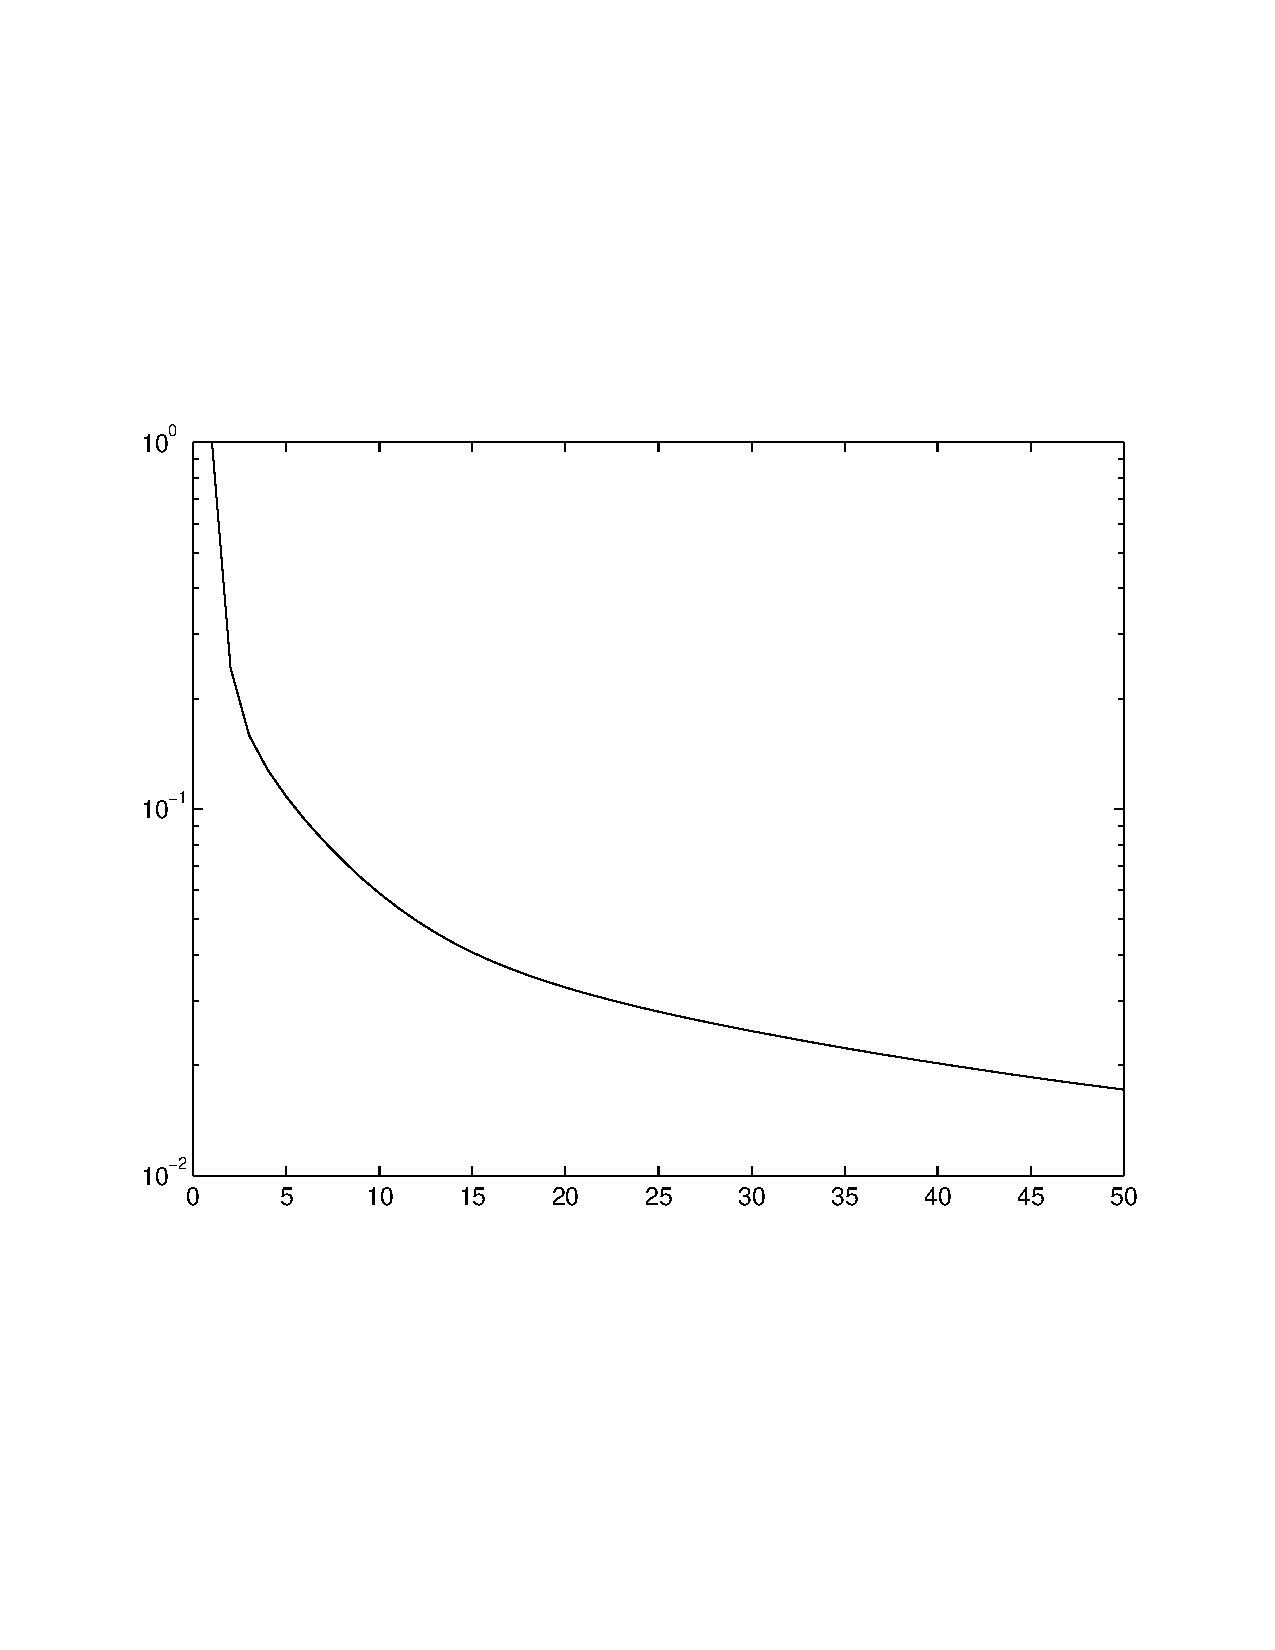
\includegraphics[height=5cm,width=3in]{pictures/richardson.pdf}
\end{center}
\caption{A picture on the GD method convergence history
\label{fig:richardson}}
\end{figure}

Our main goal is to find a way to speed up such kind of rather slowly
convergent iterative scheme.  To do that, we need to study its
convergent property in more microscopic level.  First of all, let us
now take a careful look at the convergence history picture and make
the following observation:
\begin{quote}
\underbar{\it Observation 1.}  The scheme converges rather fast in the
very beginning but then slows down after a few steps. Overall, the method 
converges very slowly. 
\end{quote}
To further understand this phenomenon, let us plot the detailed
pictures of the error functions in the first few iterations.
After a careful look at these pictures, we have the following 
observation:
\begin{quote}
\underbar{\it Observation 2.} The scheme not only converges fast in the
first few steps, but also smooth out the error function very quickly.
\end{quote}

\begin{figure}[!htb]
\begin{center}
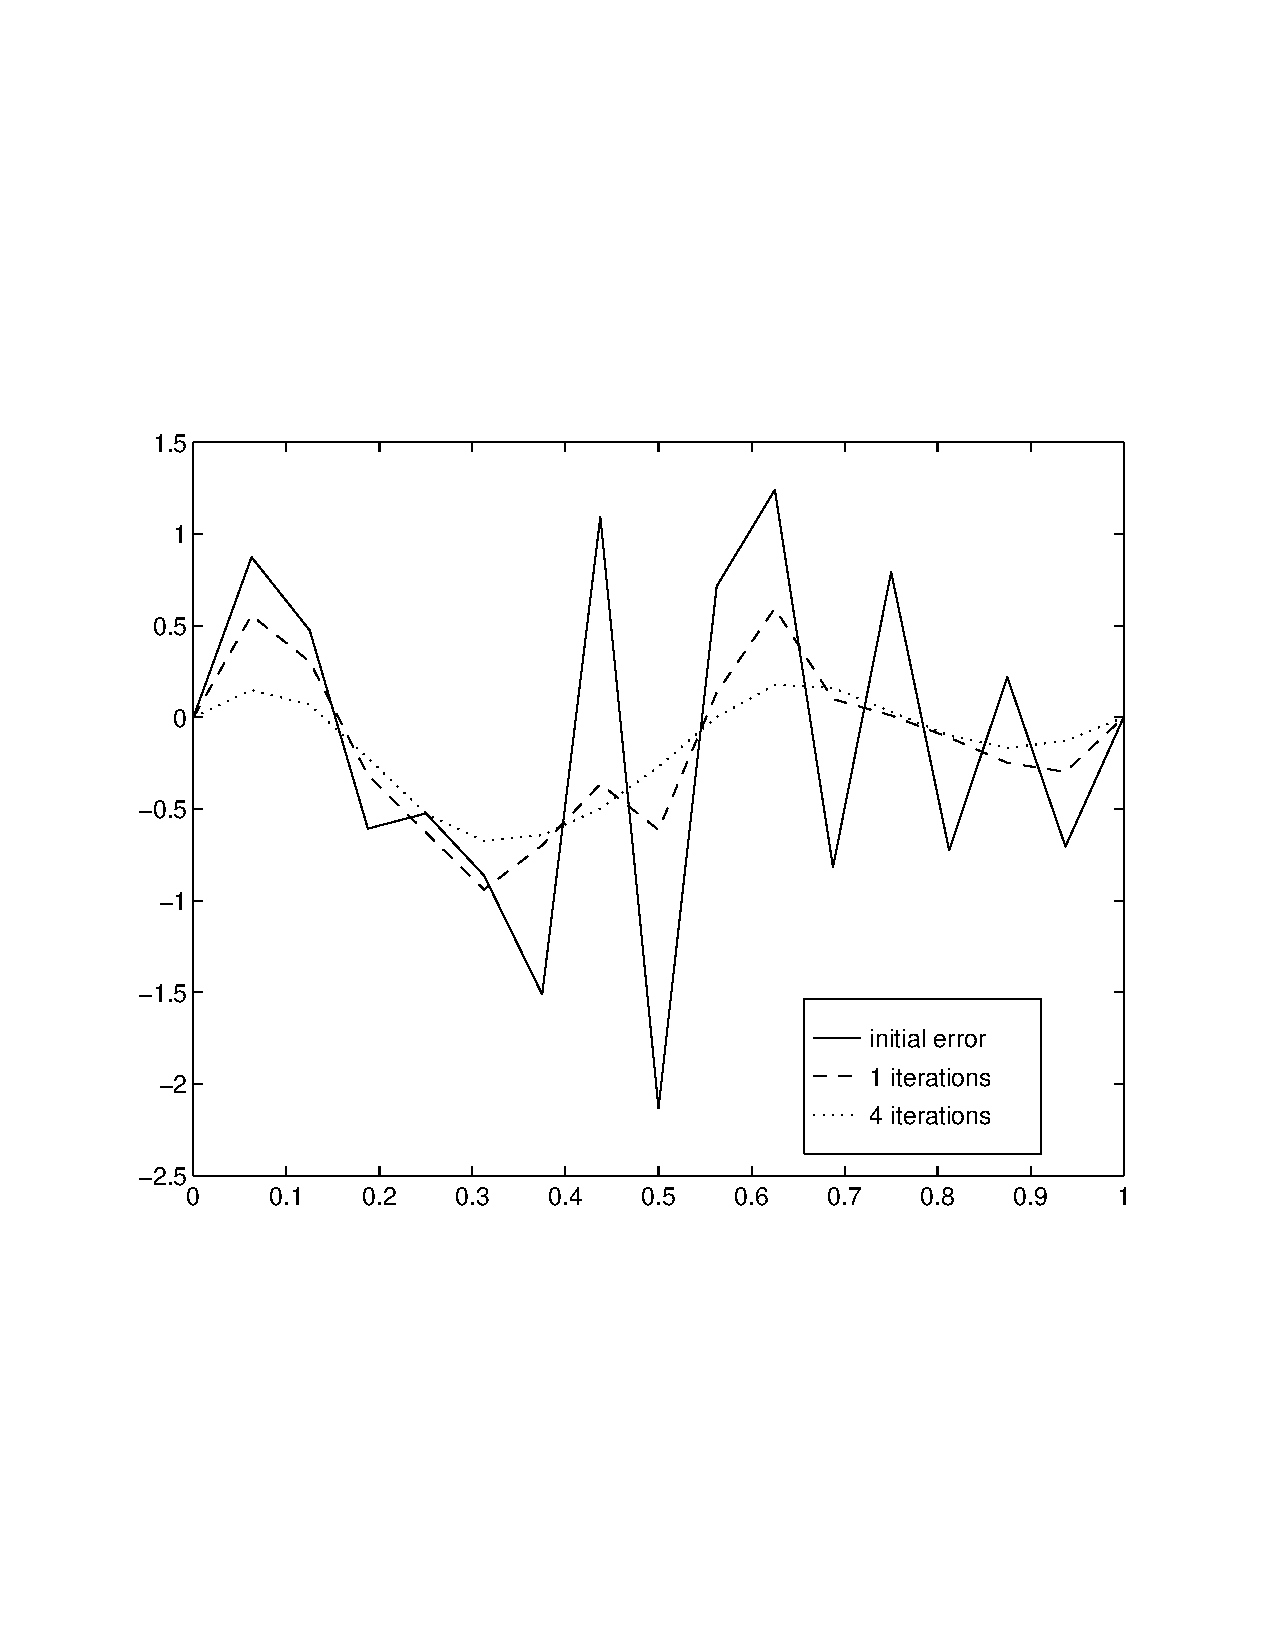
\includegraphics[height=5cm,width=3in]{pictures/smoothing.pdf}
\end{center}
\caption{The smoothing effect of the gradient descent method
\label{fig:smoothing}}
\end{figure}


In other words, the error function becomes a much smoother function
after a few such simple iterations.  This property of the iterative
scheme is naturally called {\it a smoothing property} and an iterative
scheme having this smoothing property is called a {\it smoother}.

The above two observations, especially the second one, concern the
most important property of the simple gradient descent method that we can
take advantage to get a much faster algorithm.


The gradient descent method can be written in terms of $S_{0}:\mathbb R^{N}\rightarrow \mathbb R^{N}$ satisfying
\begin{equation}
\label{jacobi1d}
\mu^{(1)}=(S_{0}b)={h\over 4} b,
\end{equation}
for equation \eqref{min} with initial guess zero.
If we apply this method twice, then
$$
\mu^{(2)}=S_1(b) = S_{0} b + S_0(b - A\ast(S_{0}b)),
$$
with element-wise form
\begin{equation} 
\begin{aligned}
\mu^{(2)}_{i} &={h\over 16}(b_{i-1}+6b_i+b_{i+1}).
\end{aligned}
\end{equation}
Then by the definition of convolution \eqref{con010}, we have
 \begin{equation}\label{eq:convS}
\mu^{(1)}= S_{0}\ast b \quad \mu^{(2)} = S_1 \ast b.
\end{equation}
with
\begin{equation}\label{eq:kernel-S1d}
S_{0} = {h\over 4},
\end{equation}
and 
\begin{equation}\label{eq:kernel-S2}
S_1={h\over 16}[1,6,1].
\end{equation} 

Hence we denote $S_0$ or $S_1$ as $S$.

Now for any given $\mu^{(0)}=\tilde{\mu}^{(0)}$, 
\begin{equation}
\begin{aligned}
&m=1,2,\cdots,2\nu\\
&\mu^{(m)}=\mu^{(m-1)}+S_0\ast(b-A\ast\mu^{(m-1)})
\end{aligned}
\end{equation}
$$\Leftrightarrow$$
\begin{equation}
\begin{aligned}
&m=1,2,\cdots,\nu\\
&\tilde{\mu}^{(m)}=\tilde{\mu}^{(m-1)}+S_1\ast(b-A\ast\tilde{\mu}^{(m-1)})
\end{aligned}
\end{equation}
we obtain $\mu^{(2\nu)}=\tilde{\mu}^{(\nu)}$ which means one step $S_1$ is equivalent to two steps of $S_0$.

\paragraph{Convergence and smoothing properties of GD}
Because of the extraordinary importance of this smoothing property, we
shall now try to give some simple theoretical analysis.  To do this,
we make use of the eigenvalues and eigenvectors of the matrix $A$.
\paragraph{Fourier analysis for the gradient descent method}
Our earlier numerical experiments indicate that the gradient descent
method has a smoothing property.  Based on our understanding of the
relation between the smoothness and the size of Fourier coefficients,
we can imagine that this smoothing property can be analyzed using the
discrete Fourier expansion.

Let $\mu$ be the exact solution of \eqref{min} and $\mu^{(m)}$ the result of
$m-th$ iteration from the gradient descent method \rf{1dRichardson}.  Then
$$
\mu-\mu^{(m)}=(1-\eta A\ast)(\mu-\mu^{(m-1)})=\ldots=(1-\eta A\ast)^m(\mu-\mu^{(0)}).
$$
Consider the Fourier expansion of the initial error:
$$
        \mu-\mu^{(0)}=\sum_{k=1}^N\alpha_k\xi^k.
$$
Then 
$$
        \mu-\mu^{(m)}=\sum_{k=1}^N\alpha_k(I-\eta A\ast)^m\xi^k.
$$
Note that $\eta=h/4$ and for any polynomial $p$
$$
p(A\ast)\xi^k=p(\lambda_k)\xi^k,
$$
we get
$$
        \mu-\mu^{(m)}=\sum_{k=1}^N\alpha_k(1-\eta\lambda_k)^m\xi^k
        =\sum_{k=1}^N\alpha_k^{(m)}\xi^k
$$
where 
$$
\alpha_k^{(m)}=\bigg(1-\sin^2{{k\pi}\over {2(N+1)}}\bigg)^m\alpha_k.
$$
For $k$ close to $N$, for example $k=N$,
note that 
$$
1-\sin^2{{N\pi}\over {2(N+1)}}=\cos^2{{N\pi}\over {2(N+1)}}
=\sin^2({\pi\over2}-{{N\pi}\over {2(N+1)}})
$$
implies
$$
|\alpha_N^{(m)}|=|\alpha_N|\sin^{2m}{{N+1-N}\over{N+1}}{\pi\over 2}
\le |\alpha_k|\bigg({{1}\over{N+1}}{\pi\over 2}\bigg)^{2m}
$$
which approaches to $0$ very rapidly when
$m\rightarrow\infty$. This means that high frequency components get
damped very quickly. 

However, for $k$ far away from $N$, for example $k=1$, note that
$$
\sin^2{{\pi}\over {2(N+1)}}\le \left({{\pi}\over {2(N+1)}}\right)^2
$$
implies
$$
|\alpha_1^{(m)}|= |\alpha_1| \bigg(1-\sin^2{{\pi}\over {2(N+1)}}\bigg)^m\ge  |\alpha_1|  \left(1-\left({{\pi}\over {2(N+1)}}\right)^2\right)^m
$$
which approaches to $0$ very slowly when
$m\rightarrow\infty$. 

This simple analysis clearly justifies the smoothing property that has
been observed by numerical experiments.

%\newpage

\begin{figure}[!ht]
\setlength{\abovecaptionskip}{0pt}
\setlength{\belowcaptionskip}{0pt}
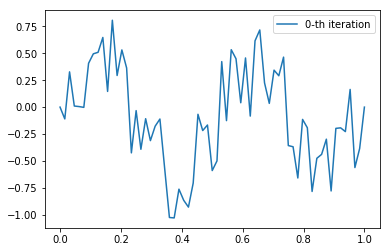
\includegraphics[width=5cm]{figures/jianhongu0.png}\qquad
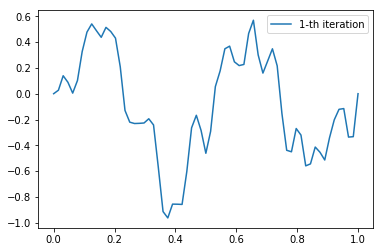
\includegraphics[width=5cm]{figures/jianhongu1.png}\qquad
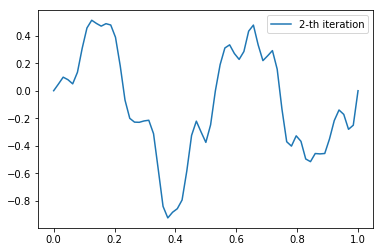
\includegraphics[width=5cm]{figures/jianhongu2.png}\qquad
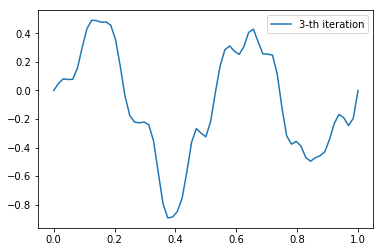
\includegraphics[width=5cm]{figures/jianhongu3.png}\qquad
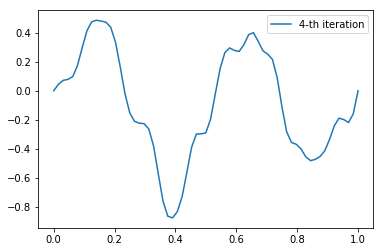
\includegraphics[width=5cm]{figures/jianhongu4.png}\qquad
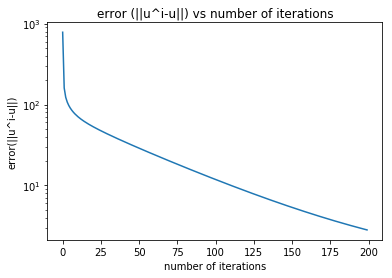
\includegraphics[width=5cm]{figures/jianhongGDerror.png}
\caption{\footnotesize{ $u-u^0$, $u-u^1$, $u-u^2$, $u-u^3$, $u-u^4$}}
\label{fig:Hmesh}
\end{figure}

%\begin{figure}[!ht] 
%\centering
%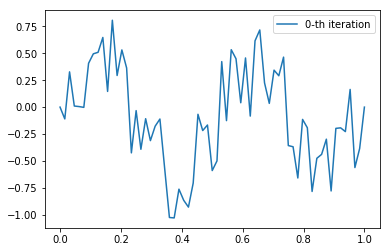
\includegraphics[width=5cm,height=4cm]{figures/jianhongu0.png}
%\caption{ $u^0$}
%\label{fig:u0j}
%\end{figure}
%\begin{figure}[!ht] 
%\centering
%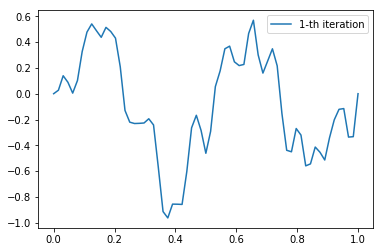
\includegraphics[width=5cm,height=4cm]{figures/jianhongu1.png}
%\caption{ $u^1$}
%\label{fig:u1j}
%\end{figure}
%\begin{figure}[!ht] 
%\centering
%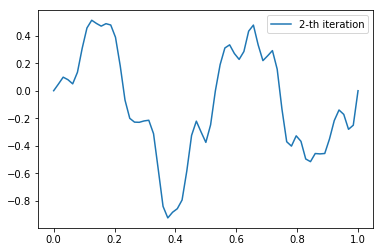
\includegraphics[width=10cm,height=8cm]{figures/jianhongu2.png}
%\caption{ $u^2$}
%\label{fig:u2j}
%\end{figure}
%\begin{figure}[!ht] 
%\centering
%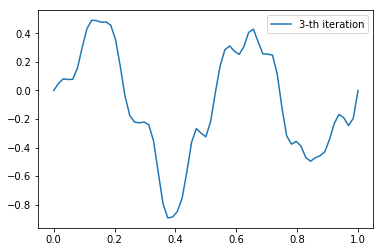
\includegraphics[width=10cm,height=8cm]{figures/jianhongu3.png}
%\caption{ $u^3$}
%\label{fig:u3j}
%\end{figure}
%\begin{figure}[!ht] 
%\centering
%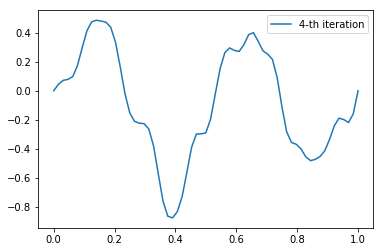
\includegraphics[width=10cm,height=8cm]{figures/jianhongu4.png}
%\caption{ $u^4$}
%\label{fig:u4j}
%\end{figure} 

\paragraph{An intuitive discussion} 
The gradient descent method is oftentimes called {\it local relaxation}
methods. This name refers to the fact that what that
algorithm does is just trying to correct the residual vector locally
at one nodal point at a time (recall that $\mu_j\approx u(x_j)$).
This local relaxation procedure is then effective to the error
components that are local in nature.  Incidentally, the nonsmooth or
high frequency component which oscillates across one or few grid
points have a strong local feature.  Therefore, it is not surprising the
 gradient descent  iteration can damp out these
nonsmooth components more easily.  This method is very inefficient
for relatively smoother components in the error since a smoother
function is more globally related in nature.


\subsection{Coarse grid correction and two grid method}
%\vspace{-1.8cm}
\begin{figure}[hpt]
\begin{center}
\includegraphics*[width=3in]{figures/twogrid.pdf}
%\vspace{-1.5cm}
\caption{Two level grids.} 
\label{Interpolation}
\end{center}
\end{figure} 

\begin{figure}[!htb]
\begin{center}
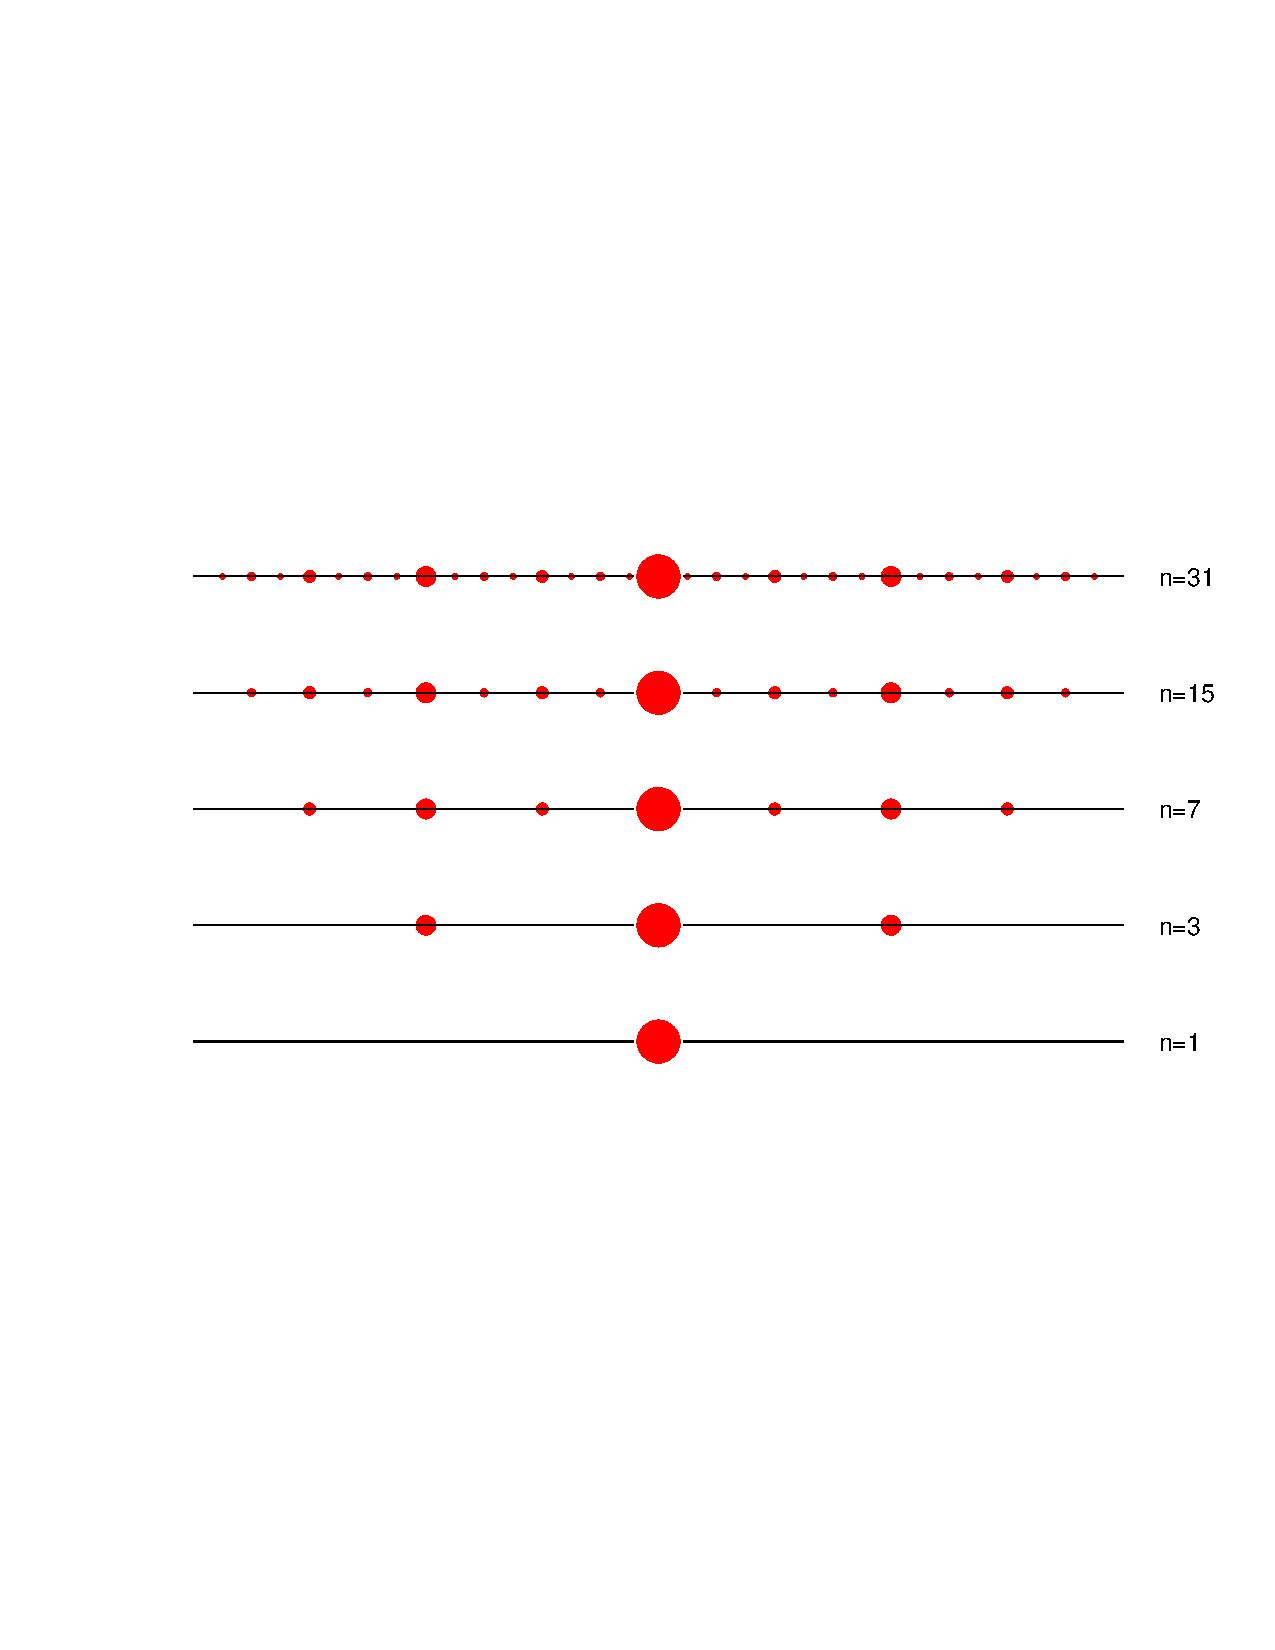
\includegraphics[width=3in]{pictures/manygr.pdf}
\end{center}
\caption{Multiple grids in one dimension
\label{fig:manygrids}}
\end{figure}

%\vspace{-0.2cm}
As we discussed earlier, although gradient descent iteration usually
converges very slowly, it does quickly smooth out the rough 
component in the error. In other words, the error becomes smooth 
after a few gradient descent iterations on a fine grid, but looks 
rough when viewed on a coarser grid. Hence, a few gradient descent
iterations can further reduce the error on the coarse grid. 
The main idea of two grid method or multigrid method is 
to use the fact that a smooth function can be well 
approximated on a coarser grid.  

In summery, we can write the two grid method in terms of finite element (FE) functions as follows:
\begin{algorithm}\caption{A two grid method (in terms of FE functions)}\Label{alg:2grid:opezero}
Input $u^0$.
\begin{enumerate}
\item [{\bf Step 1:}] Apply $\nu_1$-times gradient descent iterations for 
$$
\min_{v^1\in V_1} J(v^1)
$$
with initial guess $u^0$ to obtain $u^1\in V_1$.
\item [{\bf Step 2:}]  Apply $\nu_2$-times gradient descent iterations for 
$$
\min_{v^2\in V_2} J(u^1+v^2)
$$
with zero initial guess to obtain $u^2\in V_2$.
\item [{\bf Step 3:}]  Update: $u=u^1+u^2$.
%\item [{\bf Step 4:}]  Stop if converge or $u^0\update u$ and continue from step 1.
\end{enumerate}
\end{algorithm}
 
\newpage

\subsubsection{Realization of step 1:} 
\smallskip\hrule \smallskip 

Step 1: Given $u^{1,0}\in V_1$, apply $\nu_1$-times gradient descent method for 
$$
\min_{v^1\in V_1} J(v^1)
$$
with initial guess $u^{1,0}$ to obtain $u^1\in V_1$.
\smallskip\hrule \smallskip 


Let $\displaystyle u^{1,0}=\sum_{i=1}^{n_1}\mu^0_i\phi_i^1,\quad v^1=\sum_{i=1}^{n_1}\nu^1_i\phi_i^1,\quad  \mu^0=\{\mu^0_i\}^{n_1}_{i=1},\quad  \nu^1=\{\nu^1_i\}^{n_1}_{i=1}$,

where $\phi^1=(\phi^1_1,\phi^1_2,\cdots,\phi^1_{n_1})$
is the nodal basis of $V_1$. 

Namely, $b^1=b, \mu^1\leftarrow \mu^0$,  for $i=1:\nu_2$ 
$$
\mu^1\leftarrow  \mu^1-\eta_1 (A_1\ast \mu^1-b^1).
$$
After $\nu_1$ iterations, we obtain updated $\mu^1$ and $\displaystyle  u^1=\sum_{i=1}^{n_1}\mu^1_i\phi_i^1$.

\subsubsection{Realization of step 2:} 
\smallskip\hrule \smallskip 
{\bf Step 2:}   Apply $\nu_2$-times gradient descent iterations for 
$$
\min_{v^2\in V_2} J(u^1+v^2)
$$
with zero initial guess to obtain $u^2\in V_2$. 
\smallskip\hrule \smallskip  
Let 
$$
u^1=\sum_{i=1}^{n_1}\mu^1_i\phi_i^1,~v^2=\sum_{i}^{n_2}\nu^2_{i}\phi^{2}_i,~\mu^1=\{\mu^1_i\}^{n_1}_{i=1}, ~ \nu^2=\{\nu^2_{i}\}^{n_2}_{i=1}.$$
We have
\begin{equation}\label{min2h} 
\begin{aligned}
J(u^1+v^2)&=\frac12\int_0^1|(u^1+v^2)'|^2dx-\int_0^1f(u^1+v^2)dx\\
&=J(u^1)+J(v^2)+\int_0^1(u^1)'(v^2)'dx\\
&=\frac12 (\mu^1)^TA_1\ast \mu^1+\frac12 (\nu^2)^TA_2\ast\nu^2-(\nu^2)^Tr^2
\end{aligned}
\end{equation}
where 
\begin{equation}
r_i^2=\int_0^1 f\phi^2_i -(u^1)'(\phi^2_i)'dx=(f,\phi^2_i)-a(u^1,\phi^2_i).
\end{equation}

Now noting that 
\begin{equation}\label{prolongation}
\phi^2_i=\frac12 \phi^1_{2i-1}+ \phi^1_{2i} +\frac12 \phi^1_{2i+1},
\end{equation}
Let $\phi^2=\{\phi^2_i\}_{i=1}^{n_2}, \phi^1=\{\phi^1_i\}_{i=1}^{n_1}$. 
Using the convolution with stride notation,  we obtain 
\begin{equation}\label{rescon}
\phi^2=R\ast_2\phi^1
\end{equation}
with $R=[\frac12,1,\frac12]$.
Furthermore, 
\begin{equation}
\begin{aligned}
r^2_i&=(f, \frac12 \phi^1_{2i-1}+ \phi^1_{2i} +\frac12 \phi^1_{2i+1})-a(u^1,  \frac12 \phi^1_{2i-1}+ \phi^1_{2i} +\frac12 \phi^1_{2i+1})\\
&\displaystyle= \frac12 b^1_{2i-1}+ b^1_{2i} +\frac12 b^1_{2i+1}- \Big(\frac12 (A_1\ast\mu^1)_{2i-1}+   (A_1\ast\mu^1)_{2i}+ \frac12(A_1\ast\mu^1)_{2i+1}\Big)\\
&\displaystyle= \frac12 (b^1-A_1\ast\mu^1)_{2i-1}+ (b^1-A_1\ast\mu^1)_{2i}+\frac12 (b^1-A_1\ast\mu^1)_{2i+1}\\
&\displaystyle= \frac12 r^1_{2i-1}+ r^1_{2i} +\frac12 r^1_{2i+1},
\end{aligned}
\end{equation}
where $r^1=b^1-A_1\ast\mu^1$.
\begin{lemma}
Using the convolution with stride notation, we have $$r^2=R\ast_2r^1$$ with $R=[\frac12,1,\frac12]$.
\end{lemma}
Therefore applying gradient descent method $\nu_2$-times for \eqref{min2h} reads: 

$r^1=b^1-A_1\ast\mu^1, r^2=R\ast_2r^1, \mu^2\leftarrow 0$,
for $i=1:\nu_2 $ 
\begin{equation}
\mu^2\leftarrow \mu^2-\eta_2(A_2\ast \mu^2-r^2). 
\end{equation}
After $\nu_2$ iterations, we obtain updated $\mu^2$ and $\displaystyle  u^2=\sum_{i=1}^{n_2}\mu^2_{i}\phi_i^2$.

\subsubsection{Realization of step 3:} 
\smallskip\hrule \smallskip 
{\bf Step 3:}  $u=u^1+u^2$. 
\smallskip\hrule \smallskip 

Let $\displaystyle  \mu^2=\{\mu^2_{i}\}^{n_2}_{i=1}, \phi^{2}=\{\phi^2_i\}^{n_2}_{i=1}$.
Therefore  $u^2=\sum\limits_{i=1}^{n_2}\mu^2_{i}\phi^2_i
=(\mu^2, \phi^2)_{l^2}$ and by \eqref{rescon} we have
\begin{equation}
\begin{split}
u^2&=(\mu^2, \phi^2)_{l^2}=(\mu^2, R\ast_2\phi^1)_{l^2}=(R\ast_2^{\top}  \mu^2,  \phi^1)_{l^2}\\
&=\sum_{i=1}^{n_1}\left(R\ast_2^{\top} \mu^2\right)_i \phi^1_i
\end{split}
\end{equation}
with $R=[\frac 12,1,\frac12]$.
\begin{lemma}
The prolongation can be written as 
$R\ast_2^T: \mathbb R^{n_2}\rightarrow \mathbb R^{n_1}$, for $\mu^2\in \mathbb R^{n_2}, (R\ast_2^T \mu^2)\in R^{n_1}$ with
$$
(R\ast_2^T \mu^2)_{2i}=\mu^2_i\quad (R\ast_2^T \mu^2)_{2i+1}=\frac 12 (\mu^2_{i+1} +\mu^2_{i}).
$$
\end{lemma}
Noting that $\displaystyle u^1=\sum_{i=1}^{n_1}\mu^1_i\phi_i^1,~\mu^1=\{\mu^1_i\}^{n_1}_{i=1}$, we obtain 
$$
\mu=\mu^1+R\ast_2^T \mu^2\quad\hbox{and}\quad u=u^1+u^2.
$$
%\newpage
Next we show how to realize the Algorithm \ref{alg:2grid:opezero} in vector and convolution form.
%\begin{algorithm}\caption{A two grid method
%$\mu = {\text{2G1}}(b; \mu^0; 2,\nu_1, \nu_2)$}
%\Label{alg:2grid:opecoze}
%Given $\mu^0$.
%\begin{enumerate}
%\item[{\bf Step1:}] 
%
%Set $b^1=b, \mu^1\leftarrow\mu^0$. 
%
%{\bf For} $i=1:\nu_1$ 
%$$
%\mu^1\leftarrow  \mu^1-\eta_1 (A_1\ast \mu^1-b^1).
%$$
%{\bf end for}
%\item [\bf{Step 2:}] Set $r^1=b^1-A_1\ast\mu^1, r^2=R\ast_2r^1,
%  \mu^2\leftarrow 0$. 
%
%{\bf For} $i=1:\nu_2 $ 
%\begin{equation}
%\mu^2\leftarrow \mu^2-\eta_2(A_2\ast \mu^2-r^2). 
%\end{equation}
%{\bf end for}
%\item [{\bf Step 3:}] Update: $\mu=\mu^1+R\ast_2^T \mu^2$.
%\end{enumerate}
%\end{algorithm}

\begin{breakablealgorithm}%[!htb]
	\caption{A two grid algorithm $\mu = {\text{2G1}}(b; \mu^0; 2,\nu_1, \nu_2)$}
\label{alg:L-Slash11d}
\begin{algorithmic}
%	 \State 
%		$$
%		u \leftarrow u^0.
%		$$
	\State Set up
		$$
		b^1 = b, \quad \mu^{1}=\mu^0. 
		$$
		\State Step 1: Smoothing and restriction from fine to coarse level (nested)
		\For{$i = 1:\nu_1$}
		\State
		\begin{equation}\label{eq:smoothing}
		\mu^{1} \leftarrow \mu^{1} + S^1 \ast (b^1 - A_1 \ast \mu^1).
		\end{equation}
		\EndFor
		\State Step 2: Form restricted residual and set initial guess:
		$$
		\mu^{2} \leftarrow 0, \quad b^{2} \leftarrow R \ast_2
                (b^1-  A_1\ast \mu^{1}), 
%A_{2} = R\ast_2 A_1 \ast (R\ast_2^\top).
		$$
		\For{$i = 1:\nu_2$}
		\State
		\begin{equation}\label{eq:smoothing}
		\mu^2 \leftarrow \mu^2+ S^2 \ast (b^2- A_2\ast \mu^2).
		\end{equation}
		\EndFor
		\State Step 3: Prolongation and restriction from coarse to fine level
		\State
		$$
		\mu^{1} \leftarrow \mu^{1} + R  \ast_2^{\top} \mu^{2}.
		$$
		\State
		$$
		\mu \leftarrow \mu^{1}.
		$$
	\end{algorithmic}
\end{breakablealgorithm}






\subsection{Multilevel coarse grid corrections and a multigrid method}
\Label{sc:mg-fd}
To describe a multigrid algorithm, we first need to have a multiple
level of grids, say $\mathcal T_\ell$ with $\ell=1:J$ and $\mathcal T_1=\mathcal T_h$ being the
finest mesh.  There are many ways to obtain multiple level of grids
and one simple definition of the grid points in $\mathcal T_\ell$ is as follows:
$$
        x_i^\ell=\frac{i}{2^{J+1-\ell}},\quad i=1,2,\cdots, N_\ell, \ell=1,2,\cdots,J,
$$
where $N_\ell=2^{J+1-\ell}-1$.  Note that $\mathcal T_{\ell-1}$ can be viewed as being obtained
by adding midpoints of the subintervals in ${\mathcal T}_{\ell}$.  For each $\ell$
the set of above nodes will be denoted by $\mathcal N_\ell$.

\begin{figure}[!htb]
\begin{center}
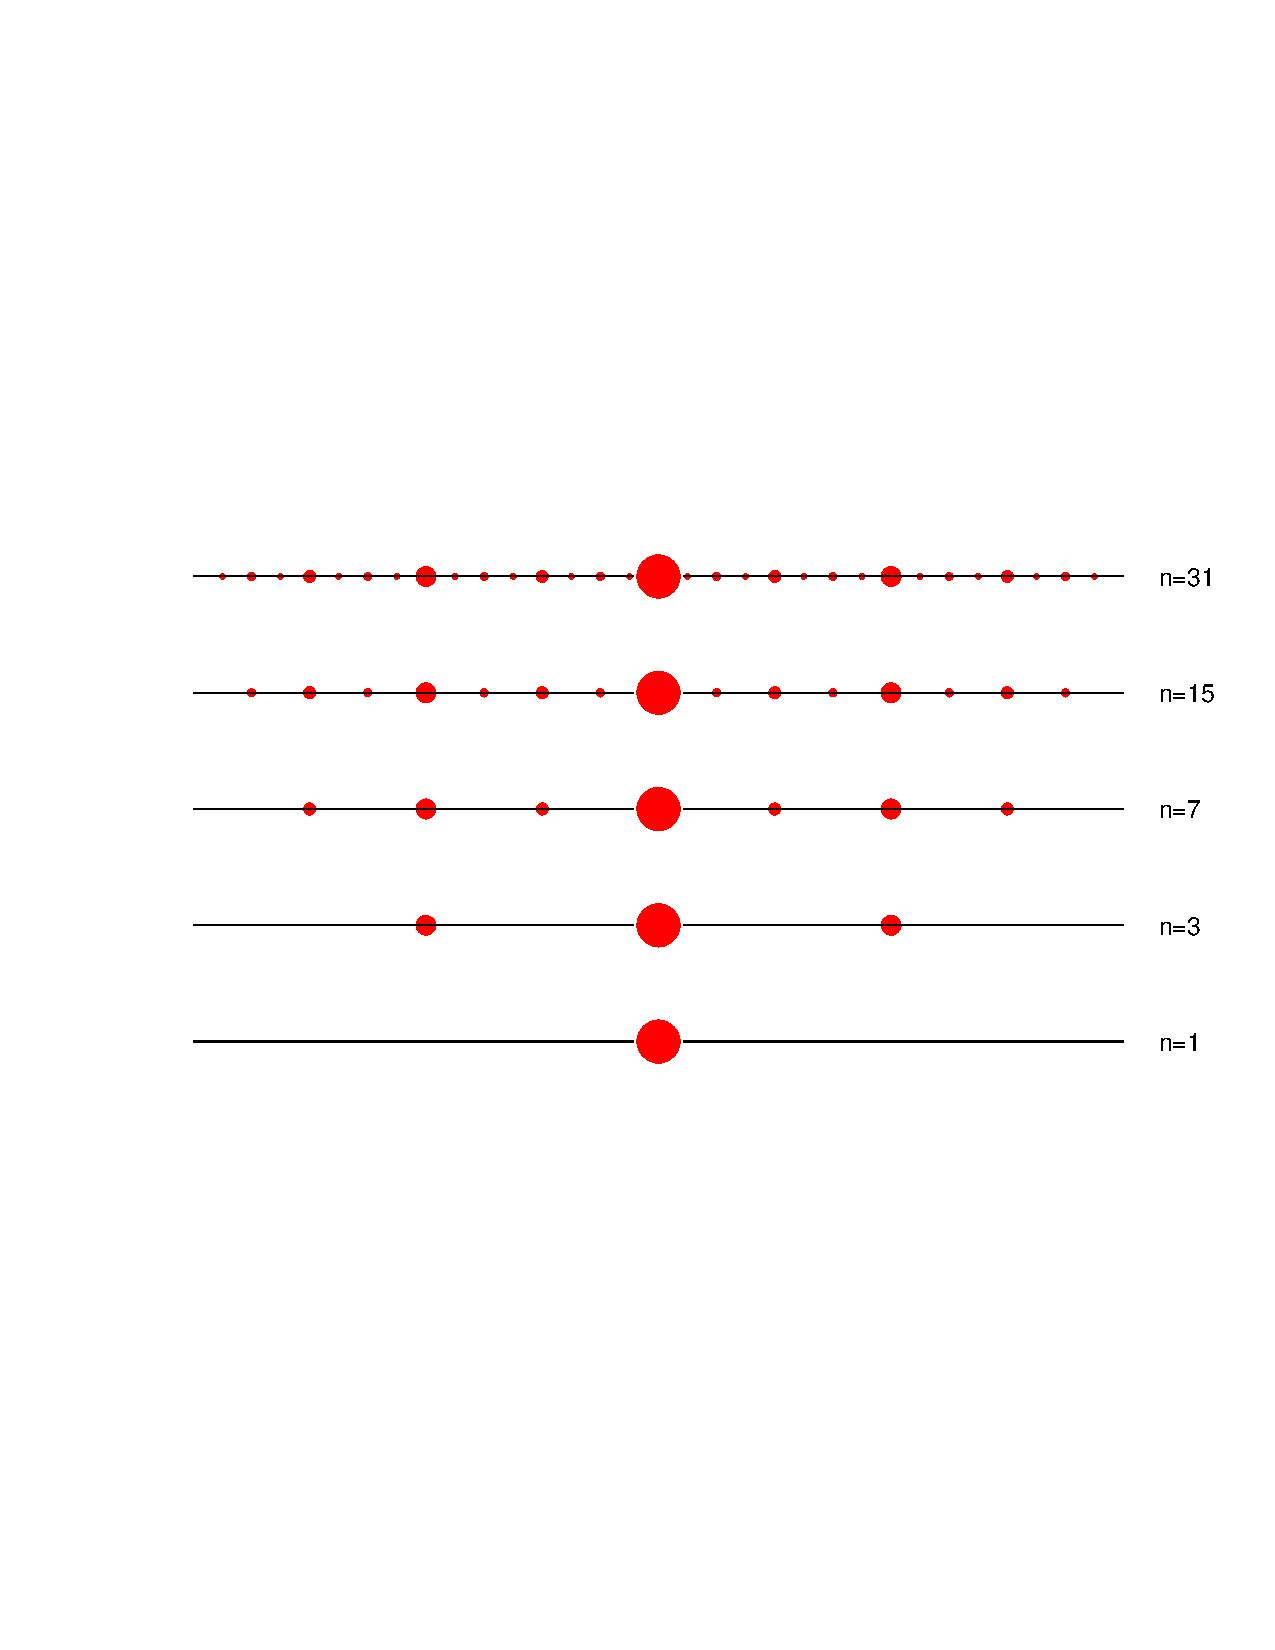
\includegraphics[width=3in]{pictures/manygr.pdf}
\end{center}
\caption{Multiple grids in one dimension
\label{fig:manygrids}}
\end{figure}


With our previous experiences in two-grid method, the description of a
multigrid method is not very difficult.  In fact, the multiple level
grids are treated by treating each two consecutive grids, say $\mathcal T_{\ell-1}$
versus $\mathcal T_{\ell}$.  If we think $\mathcal T_{\ell-1}$ versus $\mathcal T_{\ell}$ like
$\mathcal T_h$ and $\mathcal T_{2h}$, then there is not much new in the multigrid
setting.


Let us give some on details the definition of the restriction and
prolongation matrices.  The restriction matrix $R_{\ell-1}^\ell: R^{N_{\ell-1}}
\mapsto R^{N_{\ell}}$ can be defined by
\begin{equation}\Label{restrictk}
\gamma^{\ell}=R_{\ell-1}^\ell\gamma^{\ell-1}: \;
\gamma^{\ell}_i={1\over2}\gamma^{\ell-1}_{2i-1}+\gamma^{\ell-1}_{2i}+{1\over2}\gamma^{\ell-1}_{2i+1}.
\end{equation}
In matrix form 
\begin{equation}
\label{1drestriction}
R_{\ell-1}^\ell=\left(
\begin{array}{ccccccccc}
\frac{1}{2}& 1&\frac{1}{2}&&&&&&\\
&&\frac{1}{2}&1&\frac{1}{2}&&&&\\
&&&&\frac{1}{2}&1&\frac{1}{2}&&\\
&&&&&&\ddots&&\\
&&&&&&\frac{1}{2}&1&\frac{1}{2}\\
\end{array}
\right)
\end{equation}
For a special case, when $N_1=7, N_2=3$, we have 
\begin{equation}
\label{1drestriction3}
R_1^2=\left(
\begin{array}{ccccccc}
\frac{1}{2}& 1&\frac{1}{2}&0&0&0&0\\
0&0&\frac{1}{2}&1&\frac{1}{2}&0&0\\
0&0&0&0&\frac{1}{2}&1&\frac{1}{2}\\
\end{array}
\right).
\end{equation}




The prolongation matrix
$P_{\ell}^{\ell-1}: R^{N_{\ell}}
\mapsto R^{N_{\ell-1}}$ can be defined as 
\begin{equation}\Label{prolongk}
~~\epsilon^{\ell-1}=P^{\ell-1}_{\ell}\epsilon^{\ell}: \; \epsilon^{\ell-1}_{2i}=\epsilon^{\ell}_i, \epsilon^{\ell-1}_{2i+1}
= {1\over~2}(\epsilon^{\ell}_i+\epsilon^{\ell}_{i+1}), \; i=1:N_{\ell}.
\end{equation}

With the restriction and prolongation matrices in hands, we can now
present a multilevel version of the earlier two-grid algorithm.  As
mentioned before, the idea is to repeat this two grid process for the
coarse grid by using an even coarser grid.  The resulting algorithm is
just a desired multigrid algorithm. 


Using the convolution with stride notation, the restriction subprocess can also be written as 
$R\ast_2: \mathbb R^{N_\ell}\rightarrow  \mathbb R^{N_{\ell+1}}$, for any $v\in \mathbb R^{N_\ell}, u=(R\ast_2 v)\in R^{N_{\ell+1}}$ with
$$
 (R\ast_2 v)_i=\frac 12 v_{2i-1} +v_{2i}+\frac 12 v_{2i+1},\quad  \mbox{namely}\quad R\ast_2v=R_{\ell-1}^\ell v
$$
where $R=[\frac 12,1,\frac12]$ and $R_{\ell-1}^\ell $ is defined by \eqref{1drestriction}.

Next 
let $u^{\ell+1}=\sum\limits_{j=1}^{n_{\ell+1}}\mu_{j}^{\ell+1}\phi^{\ell+1}_{j}
=(  \mu^{\ell+1}, \phi^{\ell+1})_{l^2}$, then we have
\begin{equation}
\begin{split}
u^{\ell+1}&=( \mu^{\ell+1}, \phi^{\ell+1})_{l^2}
=( \mu^{\ell+1}, R\ast_2\phi^{\ell})_{l^2}=(R\ast_2^{\top} \mu^{\ell+1}, \phi^{\ell})_{l^2}\\
&=\sum\limits_{j=1}^{n_{\ell}}\left(R\ast_2^{\top} \mu^{\ell+1}\right)_{j}\phi^{\ell}_{j}.
\end{split}
\end{equation}
The prolongation subprocess can be written as 
$R\ast_2^T: \mathbb R^{N_{\ell+1}}\rightarrow \mathbb R^{N_\ell}$, for any $v\in \mathbb R^{N_{\ell+1}}, u=(R\ast_2^T v)\in R^{N_\ell}$ with
$$
(R\ast_2^T v)_{2i}=v_i,\quad (R\ast_2^T v)_{2i+1}=\frac 12 (v_{i+1} +v_i),\quad  \mbox{namely}\quad R\ast_2^Tv=P^{\ell-1}_\ell v
$$
where $R=[\frac 12,1,\frac12]$.

Using the convolution notation, the subprocess to apply $A_\ell$ to 
a vector $v\in \mathbb R^{N_\ell}$ can be written as
$A_\ell\ast: \mathbb R^{N_\ell}\rightarrow \mathbb R^{N_\ell}$, for any $v\in \mathbb R^{N_\ell}, r=(A_\ell\ast v)\in R^{N_\ell}$ with
$$
(A_\ell\ast v)_{i}=\frac{1}{h_\ell}( -v_{i-1}+2v_i-v_{i+1})
$$
where $A_\ell=\frac{1}{h_\ell}[-1,2,-1]$.

\newpage

\begin{breakablealgorithm}%[!htb]
	\caption{A multigrid algorithm $\mu = {\text{MG1}}(b; \mu^0; J,\nu_1, \cdots, \nu_J)$}
\label{alg:L-Slash11dm}
\begin{algorithmic}
%	 \State 
%		$$
%		u \leftarrow u^0.
%		$$
	\State Set up
		$$
		b^1 = b, \quad \mu^{1}=\mu^0. 
		$$
		\State Smoothing and restriction from fine to coarse level (nested)
		\For{$\ell = 1:J$}
		\For{$i = 1:\nu_\ell$}
		\State
		\begin{equation}\label{eq:smoothing}
		\mu^{\ell} \leftarrow \mu^{\ell} + S^\ell \ast (b^\ell - A_\ell \ast \mu^{\ell}).
		\end{equation}
		\EndFor
		\State Form restricted residual and set initial guess:
		$$
		\mu^{\ell+1} \leftarrow 0, \quad b^{\ell+1} \leftarrow R \ast_2 (b^\ell -  A_\ell \ast \mu^{\ell}), A_{\ell+1} = R       \ast_2 A_\ell \ast (R\ast_2^\top).
		$$
		\EndFor
		\State Prolongation and restriction from coarse to fine level
		\For{$\ell = J-1:1$}
		\State
		$$
		\mu^{\ell} \leftarrow \mu^{\ell} + R  \ast_2^{\top} \mu^{\ell+1}.
		$$
%		%		\IF{V-cycle}
%		\For{$i = 1:\nu_\ell$}
%		\State
%		$$
%		u^{\ell,i} \leftarrow u^{\ell,i-1} + [B^{\ell,i}]^T (f^\ell - A^{\ell} u^{\ell,i-1})
%		$$
%		\EndFor
%		%		\ENDIF
		\EndFor
		\State
		$$
		\mu \leftarrow \mu^{1}.
		$$
	\end{algorithmic}
\end{breakablealgorithm}


Application of Multigrid:
		Given $\mu^{(0)}$, for $m=1,2,\cdots$ till convergence
		$$
		\mu^{(m)}= {\text{MG1}}(b; \mu^{{(m-1)}}; J,\nu_1, \cdots, \nu_J).
		$$
		
\example Let $f(x)=1$. Consider 
\begin{equation}\label{1Dposi}
\left\{
\begin{aligned}
-u''&= f, \,\, 0<x<1, \\
 u(0)&=u(1)=0.
\end{aligned}
\right.
\end{equation}
The true solution $u=\frac12 x(1-x)$. Given the partition with the grid points 
$x_i=\frac{i}{n+1}, i=0,1,\cdots,n+1$, then by finite element discretization, 
we obtain 
\begin{equation}\label{matrix}
A\ast \mu =b, A=\frac{1}{h}[-1,2,-1].
\end{equation}
Use gradient descent method and multigrid to solve \eqref{matrix} with random initial guess $\mu^0$.



\begin{figure}[!ht]
\centering
\setlength{\abovecaptionskip}{0pt}
\setlength{\belowcaptionskip}{0pt}
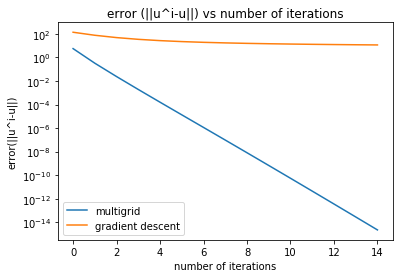
\includegraphics[width=8.3cm]{figures/mgcompare.png}
\caption{Comparison GD with Multigrid}
\label{fig:Hmesh}
\end{figure}






%\input{3FEM/1DMGvector}
\clearpage
\subsection{Comparison between 1D and 2D finite element discretization}
\begin{table}[]
\centerline{\bf 1D and 2D Comparison for Finite Element and Multigrid }\medskip
\centering
\begin{tabular}{ p{7cm}<{\centering}|p{7cm}<{\centering}}
\hline
%\smallskip 
   $1D: \Omega=(0, 1)$      \smallskip &    $2D: \Omega=(0, 1)\times (0, 1)$     
%\smallskip 
  \\\hline
 $\begin{cases}
 -u''=f&x\in \Omega\\
 u(0)=u(1)=0&
 \end{cases}$        &     
 $\begin{cases}
 -\triangle u=f&x\in \Omega\\
 u=0&x\in \partial \Omega
 \end{cases}$       
 \\\hline
  \multicolumn{2}{c}{$\displaystyle u=\argmin_{v\in V}   J(v)$}   
 \\\hline
  $\displaystyle J(v)={1\over 2}\int_0^1  |v'|^2dx - \int_0^1  fv dx $
  &     $\displaystyle J(v)={1\over 2}\int_\Omega  |\nabla v|^2dx - \int_\Omega fv
  dx $      
 \\\hline
 \multicolumn{2}{c}{$V=\{v: \Omega\rightarrow \mathbb{R} \mbox{ is continuous and piecewise smooth, } v|_{\partial \Omega}=0\}$}
 \\\hline 
  \multicolumn{2}{c}{FE space: $V_h=\{v_h\in V, v_h \mbox{ is piecewise linear w.r.t. } \mathcal{T}_h\}$}  
\\\hline
\begin{minipage}{0.5\textwidth}\centering
      	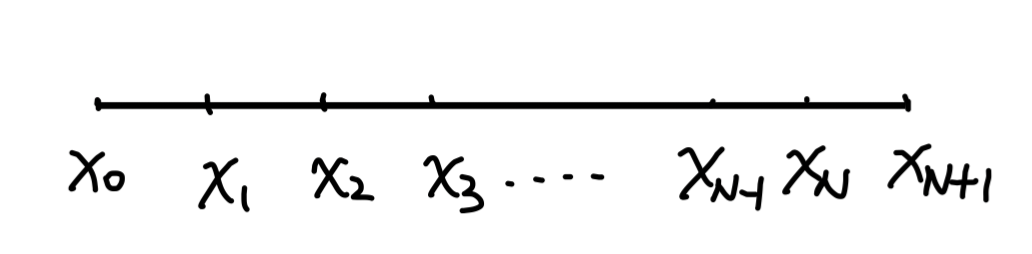
\includegraphics[width=4cm]{figures/grid1d.png}
   	 \end{minipage}  
    	&  
	\begin{minipage}{0.2\textwidth}\centering
      	\includegraphics[width=2cm]{figures/grid1.png}
   	 \end{minipage} 
\\\hline
 $\phi_i(x)$   & $\phi_{ij}(x, y)$ 
 \\\hline
 \begin{minipage}{0.4\textwidth}\centering
      	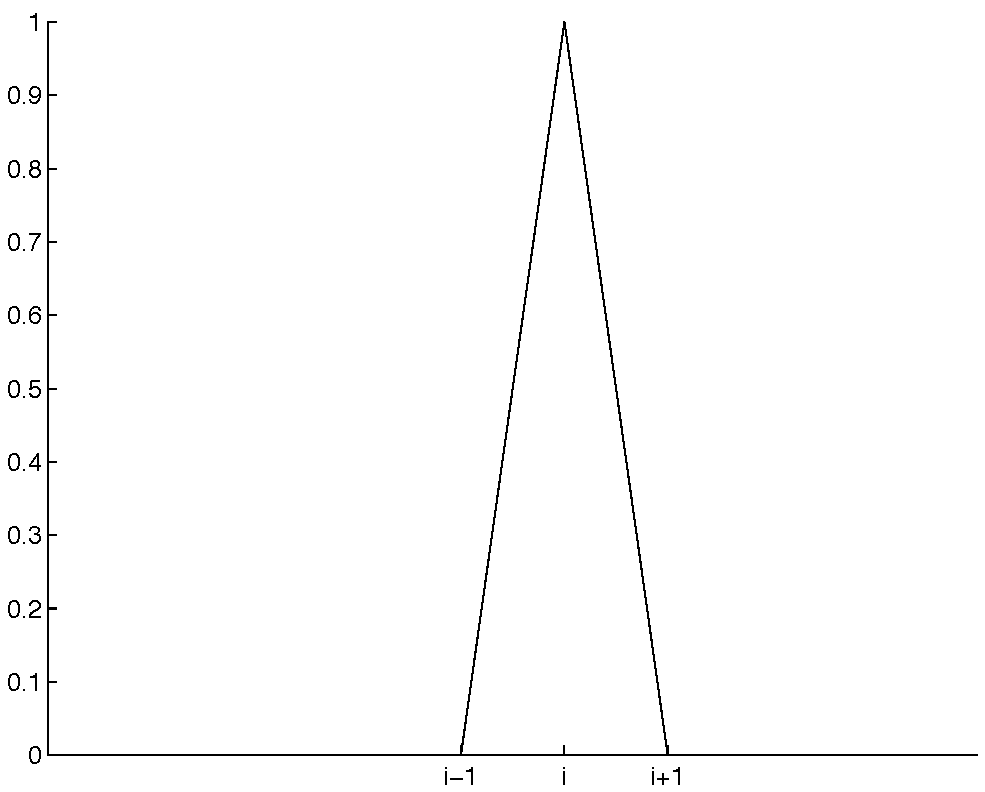
\includegraphics[height=2cm]{figures/basisfunction.pdf}
   	 \end{minipage}
    & \begin{minipage}{0.5\textwidth}\centering
      	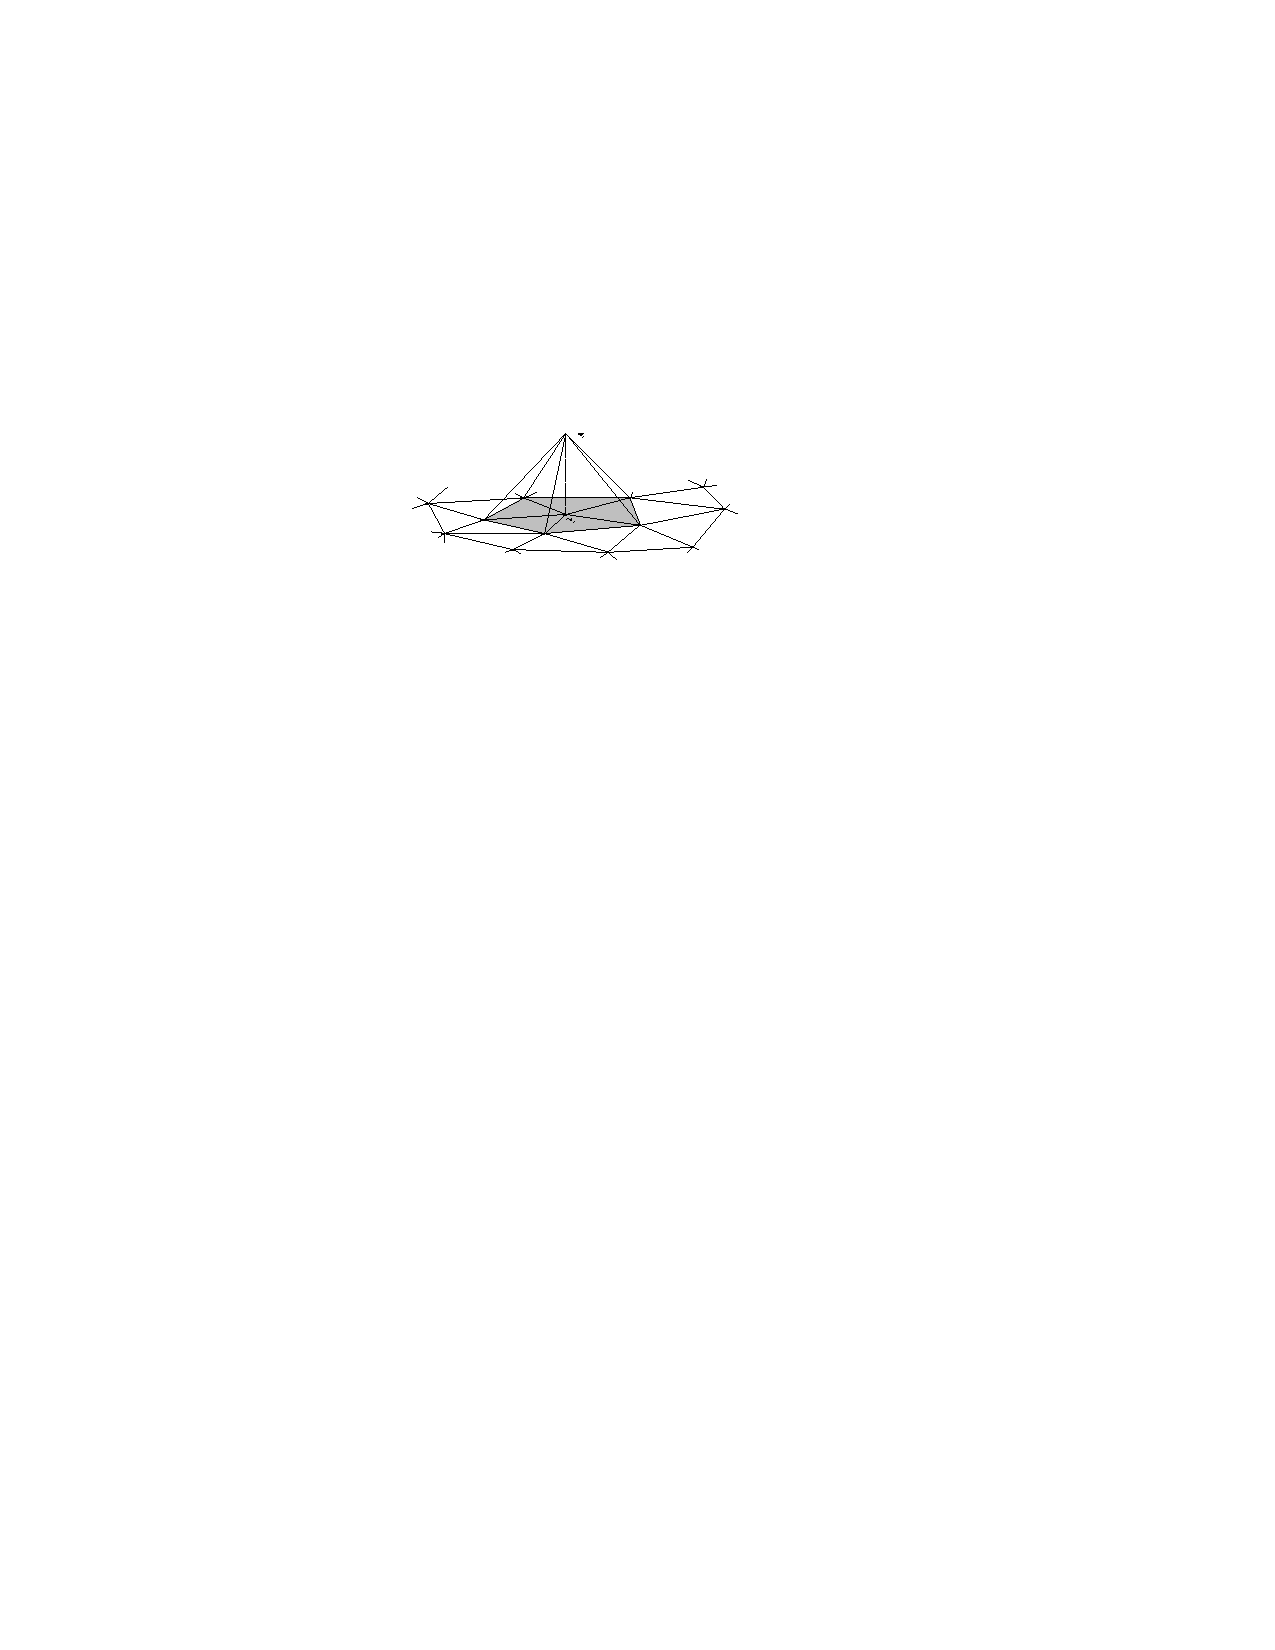
\includegraphics[height=2cm]{figures/nodalbasis.pdf}
   	 \end{minipage} 
\\\hline
 \multicolumn{2}{c}{Find $u_h\in V_h$ s.t. $\displaystyle J(u_h)=\min_{v_h\in V_h} J(v_h)$}    
 \\\hline
 $\displaystyle u_h=\sum_{i=1}^n \mu_i\phi_i(x)$         &    $\displaystyle u_h=\sum_{i, j=1}^n \mu_{ij}\phi_{ij}(x, y)$      
  \\\hline
 Find $\mu\in \mathbb{R}^n$ s.t. $\displaystyle  I(\mu)=\min_{\nu\in \mathbb{R}^n} I(\nu)$
 &   Find $\mu\in \mathbb{R}^{n\times n}$ s.t. $\displaystyle  I(\mu)=\min_{\nu\in \mathbb{R}^{n\times n}} I(\nu)$  
 \\\hline
 \multicolumn{2}{c}{$I(\nu)={1\over 2}(A\ast \nu, \nu)_{l^2} - (b, v)_{l^2} $}  
 \\\hline
 $A={1\over h}(-1, 2, -1)$        &   
$\scriptsize
 A=\begin{pmatrix}
 0&-1&0\\
 -1&4&-1\\
 0&-1&0
 \end{pmatrix}
$     
 \\\hline
  \multicolumn{2}{c}{$\mu=\argmin I(\nu) \Longleftrightarrow \nabla J(\mu)=A\ast \mu -b=0$}    \\\hline
\multicolumn{2}{c}{ GD Method:   $ \mu^{(m+1)}=\mu^{(m)} -\eta(A\ast \mu^{(m)}-b)$}       
 \\\hline
$\eta={h\over 4}$       &    $\eta={1\over 8}$      \\\hline
\end{tabular}
\end{table}

\renewcommand\arraystretch{2}
\begin{table}[]
\centerline{\bf Basic multigrid components}
\medskip 
\centering
\begin{tabular}{ p{7cm}<{\centering}|p{7cm}<{\centering}}
\hline 
 \begin{minipage}{0.5\textwidth}
      	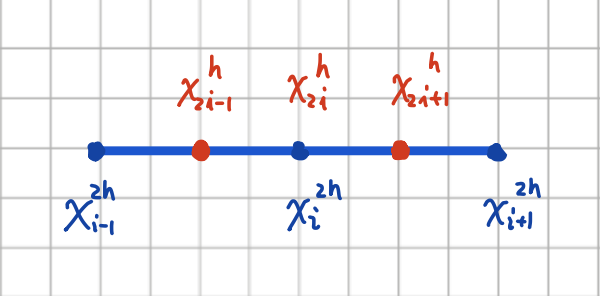
\includegraphics[width=7cm,height=3.5cm]{figures/two-grids1.png}
   	 \end{minipage}
    & \begin{minipage}{0.5\textwidth}
      	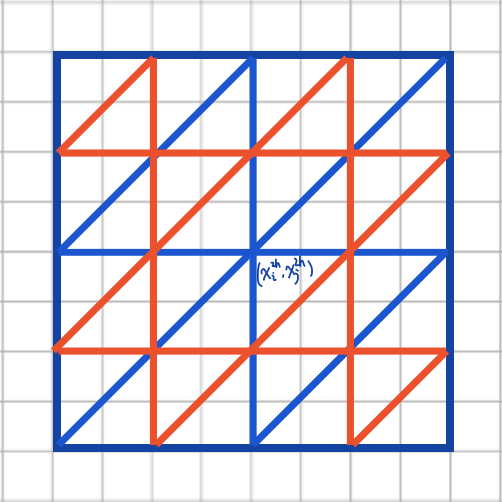
\includegraphics[width=7cm,height=7cm]{figures/two-grids2.png}
   	 \end{minipage} 
\\\hline
  $\phi_{i}^{2h}={1\over 2} \phi_{2i-1}^{h} + \phi_{2i}^{h} + {1\over 2} \phi_{2i+1}^{h}$        &     { \small$ \phi_{i,j}^{2h} =\phi_{2i,2j}^{h} 
+\frac{1}{2}\left(\phi_{2i-1,2j-1}^{h} +\phi_{2i+1,2j+1}^{h} \right)
+\frac{1}{2}\left(\phi_{2i-1,2j}^{h} +\phi_{2i,2j-1}^{h} 
+\phi_{2i+1,2j}^{h} +\phi_{2i,2j+1}^{2h} \right)$}
      \\\hline
  \multicolumn{2}{c}{ $\Phi^{2h}=R\ast_2 \Phi^h$  }    \\\hline
 $R=({1\over 2}, 1, {1\over 2})$      &   $R=\begin{pmatrix}
0&{1\over 2}&{1\over 2}\\
{1\over 2}&1&{1\over 2}\\
{1\over 2}&{1\over 2}&0
\end{pmatrix}$       \\\hline
\end{tabular}
\end{table}

\clearpage




%%%%%%%%%%%%%%%%%%%%%%%%%%%%%%%%%%

\section{Finite element method and convolution}\label{sec:mg}
Let us first briefly describe finite
element methods for the numerical solution of the following boundary
value problem
\begin{equation}
\label{laplace}
-\Delta u = f,  \mbox{ in } \Omega,\quad
u=0  \mbox{ on } \partial\Omega,\quad
\Omega=(0,1)^2.
\end{equation}
For the $x$ direction and the $y$ direction, we consider the partition:
\begin{equation}\label{partitionyx}
 0=x_0<x_1<\cdots<x_{n+1}=1, \quad x_i=\frac{i}{m+1},\quad (i=0,\cdots,m+1);
 \end{equation}
 \begin{equation}\label{partitiony}
 0=y_0<y_1<\cdots<y_{n+1}=1, \quad y_j=\frac{j}{n+1},\quad (j=0,\cdots,n+1).
\end{equation}
For $\Omega=(0,1)^2$, we just choose $m=n$. Such a uniform partition in the $x$ and $y$ directions leads us to a special example in two dimensions, a uniform square mesh $\R_h^2 = \big\{(ih,jh); i, j \in \Z\big\}$ (Figure \ref{fig:2dpartition}). 


\begin{figure}
\begin{center}
\setlength{\unitlength}{0.5mm}
\begin{picture}(45,45)(50,0)
\linethickness{0.25mm}
\multiput(0,0)(10,0){6}{\line(0,1){50}}
\multiput(0,0)(0,10){6}{\line(1,0){50}}
\put(0,0){\line(1,1){50}}
\put(10,0){\line(1,1){40}}
\put(20,0){\line(1,1){30}}
\put(30,0){\line(1,1){20}}
\put(40,0){\line(1,1){10}}
\put(0,10){\line(1,1){40}}
\put(0,20){\line(1,1){30}}
\put(0,30){\line(1,1){20}}
\put(0,40){\line(1,1){10}}
\put(47,34){$\displaystyle \left. \begin{array}{l}~ \\ ~\end{array}
\right\} h={1\over n+1}$}
\put(54,14){$\displaystyle N = n^2$}
\multiput(100,0)(10,0){6}{\line(0,1){50}}
\multiput(100,0)(0,10){6}{\line(1,0){50}}
\put(147,34){$\displaystyle \left. \begin{array}{l}~ \\ ~\end{array}
\right\} h={1\over n+1}$}
\put(154,14){$\displaystyle N = n^2$}
\end{picture}
\setlength{\unitlength}{0.5mm}
\end{center}
\label{fig:2dpartition}
\caption{Two-dimensional uniform grids for finite element}
\end{figure}

We consider two finite elements: continuous linear element and
bilinear element. These two finite element methods find $u_h\in V_h$
such that
\begin{equation}\label{Discrete:2d}
(\nabla u_h, \nabla v_h)=(f, v_h),\ \forall v_h\in V_h.
\end{equation}


Basis functions $\phi_{ij}$ satisfy 
\begin{equation}
  \label{NodalBasis}
\phi_{ij}(x_k,y_l)=\delta_{(i,j),(k,l)}.  
\end{equation}

Consider continuous linear finite element discretization of \eqref{laplace} on
the left triangulation in Fig \ref{fig:2dpartition}. The discrete
space for linear finite element is
$$
\mathcal V_h=\{v_h: v_h|_K\in P_1(K) \text{ and } v_h \text{ is globally continuous}\}.
$$ 

By simple computation, we have
\begin{equation}
(\nabla \phi_{i,j} , \nabla \phi_{k,l})=
\left\{
		\begin{array}{ll}
		-1 & \mbox{ if } |k-i|+|j-l|= 1,\\     
		4 & \mbox{ if } (k,l)=(i,j),\\
		0& \mbox{ elsewhere}.
		\end{array}
		\right.
\end{equation}
It is easy to verify that the formulation for the linear element method is 
\begin{equation}
  \label{2d-fe0}
A\ast u=4u_{i,j}-(u_{i+1,j}+u_{i-1,j}+u_{i,j+1}+u_{i,j-1})=f_{i,j},~~u_{i,j}=0~~\hbox{if}~~i ~~\hbox{or}~~ j\in \{0, n+1\},
\end{equation}
where 
\begin{equation}\label{fij_fe}
f_{i,j} = \int_{\Omega} f(x,y)\phi_{i,j}(x,y) {\rm d}x {\rm d}y \approx h^2 f(x_i, y_j).
\end{equation} 

\begin{definition}\label{def:convolution}
A convolution defined on $\mathbb{R}^{m\times n}$ is a linear mapping 
$K\ast: \mathbb{R}^{m\times n}\mapsto \mathbb{R}^{m\times n}$ defined with padding,  
for any $g \in \mathbb{R}^{m\times n}$ by:
%We first consider $\theta$ a convolution operator (with stride $1$) 
%and padding:
\begin{equation}\label{con010}
[K \ast g]_{i,j} = \sum_{p,q=-k}^k K_{p, q} g_{i + p, j + q}, \quad i=1:m, j = 1:n.
\end{equation}
\end{definition}
The coefficients in \eqref{con010} constitute  a kernel matrix
\begin{equation}
K \in \mathbb{R}^{(2k+1) \times (2k+1)},
\end{equation}
where $k$ is often taken as a small integer. 
Here we note that the indices for the entries in $K$ are given in a special way. 
For example, if $k=1, K\in \mathbb R^{3\times 3}$, and 
$$
K=\begin{pmatrix}
	K_{-1,-1} &K_{-1,0} &K_{-1,1} \\
	K_{0,-1} &K_{0,0} &K_{0,1} \\
	K_{1,-1} &K_{1,0} &K_{1,1} \\
	\end{pmatrix},
$$
for we may have the following 2D Laplacian kernel
\begin{equation}\label{key}
K=\begin{pmatrix}
0 &-1 &0\\
-1 &4&-1 \\
0 &-1 &0 \\
\end{pmatrix}.
\end{equation}  
Here padding means how $ g_{i+ p, j + q}$ is defined
when $(i+ p, j + q)$ is out of $1:m$ or $1:n$. 
The following three choices are often used
\begin{equation}\label{eq:padding}
g_{i + p, j + q} = \begin{cases}
0,  \quad &\text{zero padding}, \\
f_{(i + p)\pmod{m}, (s + q)\pmod{n}},  \quad &\text{periodic padding}, \\
f_{|i-1 +p|, |j -1  +q|},  \quad &\text{reflected padding}, \\
\end{cases}
\end{equation}
if 
\begin{equation}
i + p \notin \{1, 2, \dots, m\} ~\text{or} ~  j+ q \notin \{1, 2, \dots, n\}.
\end{equation}
Here $ d \pmod{m} \in \{1, \cdots, m\} $  means the remainder when $d$ is divided by $m$.

\begin{definition}\label{def:convolution2}
For $g \in \mathbb{R}^{m\times n}$, convolution with stride $2$ is defined as 
\begin{equation}\label{stride_2}
[K \ast_2 g]_{i,j} = \sum_{p,q=-k}^k K_{p,q} g_{2i + p-1, 2j + q-1},  
\quad i = 1: \lfloor \frac{m+1}{2}\rfloor , j = 1: \lfloor \frac{n+1}{2} \rfloor.
\end{equation}
\end{definition}

Using the convolutional notation \eqref{con010}, \eqref{2d-fe0} can be written as 
\begin{equation}
  \label{eq:Ac}
A\ast u=f
\end{equation}
with 
\begin{equation}
  \label{Ac}
A=
\begin{pmatrix}
0&-1&0\\
-1&4&-1\\
0&-1&0
\end{pmatrix}
.
\end{equation}

\begin{proposition}\label{prop:A}
The mapping $A\ast$ has following properties
\begin{enumerate}
\item $A$ is symmetric, namely 
$$
(A\ast u, v)_{l^2}=(u,A\ast v)_{l^2}.
$$
\item  $(A\ast v, v)_F>0, ~~~\hbox{if}~~~v\neq 0.$
\item $A\ast u=f$ if and only if 
\begin{equation}\label{minProblem}
u\in \argmin_{v\in \mathcal V_h} J(v)={1\over 2}(A\ast v,v)-(f,v).
\end{equation}
\item The eigenvalues $\lambda_{kl}$ and eigenvectors $u^{kl}$ of $A$ are given by
$$
\lambda_{kl}=4(\sin^2\frac{k\pi}{2(n+1)}+ \sin^2\frac{l\pi}{2(n+1)}),
$$
$$
u_{ij}^{kl}=\sin \frac{ki\pi}{n+1}\sin \frac{lj\pi}{n+1},\ 1\leq i\leq n,\ 1\leq j\leq n,
$$
and  $\rho(A)<8$. Furthermore,
\begin{equation*}
\lambda_{n,n}=8\cos^2\frac{\pi}{2(n+1)}\approx 8(1- ({\pi\over 2(n+1)})^2) \approx 8-{2\pi^2\over (n+1)^2}
\end{equation*}
\end{enumerate}
\end{proposition}


  





%\subsection{Bilinear element}

%\noindent\textbf{Bilinear element}

Continuous bilinear finite element discretization of
\eqref{laplace} on the right mesh in 
Fig. \ref{fig:2dpartition}. The discrete space for linear finite element is 
$$
\mathcal V_h=\{v_h: v_h|_K\in \{1,\ x,\ y,\ xy \} \text{ and } v_h \text{ is globally continuous}\}.
$$ 
%It is easy to see that on the element $K$ with four vertice $(x_i, y_j)$, $(x_i,y_{j+1})$, $(x_{i+1},y_j)$ and $(x_{i+1},y_{j+1})$, the nodal basis functions 
%%associate with each $(x_i,y_j)$   
%(satisfying \eqref{NodalBasis}) are given by 
%\begin{equation}
%  \label{BilinearNodalBasis}
%  \begin{array}{llll}
%\phi_{i,j}(x,y)&=  \frac{(x_{i+1}-x)(y_{j+1}-y)}{h^2}, 
%&\phi_{i, j+1}(x,y)&= \frac{(x_{i+1}-x)(y-y_j)}{h^2}, \\
%\phi_{i+1,j}(x,y)&=  \frac{(x-x_i)(y_{j+1}-y)}{h^2}, 
%& \phi_{i+1,j+1}(x,y)&= \frac{(x-x_i)(y-y_j)}{h^2}.
%\end{array}
%\end{equation}
For bilinear element case, we have 
\begin{equation}
\begin{split}
(\nabla \mathbf u_h, \nabla \mathbf v_h)&=\sum\limits_{i,j=1}^{n}\int_{E_{i,j}}\nabla \mathbf u_h, \nabla \mathbf v_h dxdy\\
&=\sum\limits_{i,j=1}^{n}\int_{E_{i,j}} \left(\frac{(u_{i+1,j}-u_{i,j})(y_{j+1}-y)}{h^2}
+\frac{(u_{i,j+1}-u_{i+1,j+1})(y-y_j)}{h^2}\right)\\
&~\qquad\qquad\left(\frac{(v_{i+1,j}-v_{i,j})(y_{j+1}-y)}{h^2}
+\frac{(v_{i,j+1}-v_{i+1,j+1})(y-y_j)}{h^2}\right)\\
&~~\quad\qquad+\left(\frac{(u_{i,j+1}-u_{i,j})(x_{i+1}-x)}{h^2}
+\frac{(u_{i+1,j}-u_{i+1,j+1})(x-x_i)}{h^2}\right)\\
&~\qquad\qquad \left(\frac{(v_{i,j+1}-v_{i,j})(x_{i+1}-x)}{h^2}
+\frac{(v_{i+1,j}-v_{i+1,j+1})(x-x_i)}{h^2}\right)dxdy\\
&=(A\ast u, v)_{l^2}.
\end{split}
\end{equation}
where $A=\left(
\begin{matrix}
-1&-1&-1\\
-1&8&-1\\
-1&-1&-1\\
\end{matrix}
\right)$ 
and $A\ast u$ is given by \eqref{2d-fe1}.

And we have
\begin{equation}
  \label{2d-fe1}
A\ast u=8u_{ij}-(u_{i+1,j}+u_{i-1,j}+u_{i,j+1}+u_{i,j-1}+u_{i+1,j+1}+u_{i-1,j-1}+u_{i-1,j+1}+u_{i+1,j-1})=f_{i,j},
\end{equation}
and 
$
u_{i,j}=0~~\hbox{if}~~i ~~\hbox{or}~~ j\in \{0, n+1\}.
$

\section{Piecewise linear functions on multilevel
  grids in 2D}\label{sec:functions}
An image can be viewed as a function on a grid.  Images with different
resolutions can then be viewed as functions on grids of different
sizes.  The use of such multiple-grids is a main technique used in the
standard multigrid method for solving discretized partial differential
equations, and it can also be interpreted as a main ingredient used in
convolutional neural networks (CNN) for image calssification.

An image can be viewed as a function on a grid \cite{krizhevsky2012imagenet} on 
a rectangle  domain $\Omega\in \mathcal R^2$.  Without loss of generality,
 we assume that the grid, $\mathcal T$, is of size
$$
m=2^{s}+1~~~n=2^{t}+1 
$$
for some integers $s, t\ge 1$.
Starting from $\mathcal T_1=\mathcal T$,  we consider a sequence of
coarse grids with $J=\min (s,t)$ (as depicted in Fig.~\ref{mgrid} with $J=4$):
\begin{equation}
\label{grids}
\mathcal T_1, \mathcal T_2, \ldots, \mathcal T_J
\end{equation}
such that ${\cal T}_\ell$ consist of $m_\ell\times n_\ell$ grid
points, with 
\begin{equation}
\label{mn-ell}
 m_\ell=2^{s-\ell+1}+1,~~ n_\ell=2^{t-\ell+1}+1.   
\end{equation}
\begin{figure}[!htbp]\label{mgrid}
	\begin{center}
		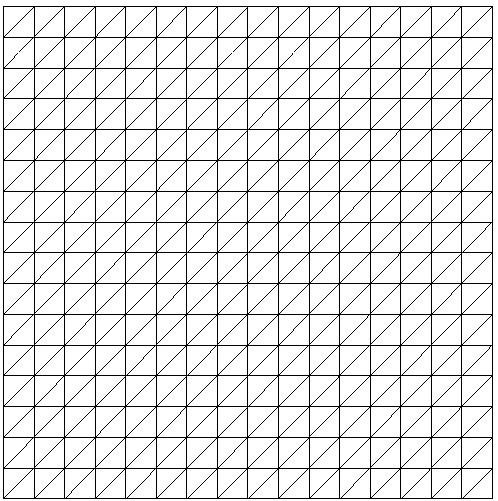
\includegraphics[width=0.15\textwidth]{grid2.png} \quad 
		\includegraphics[width=0.15\textwidth]{grid1.png} \quad 
		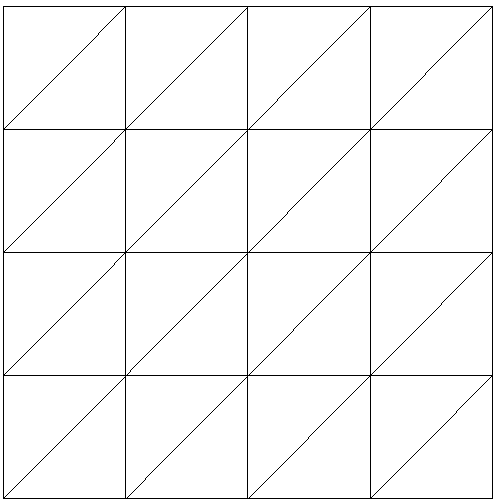
\includegraphics[width=0.15\textwidth]{grid0.png} \quad 
		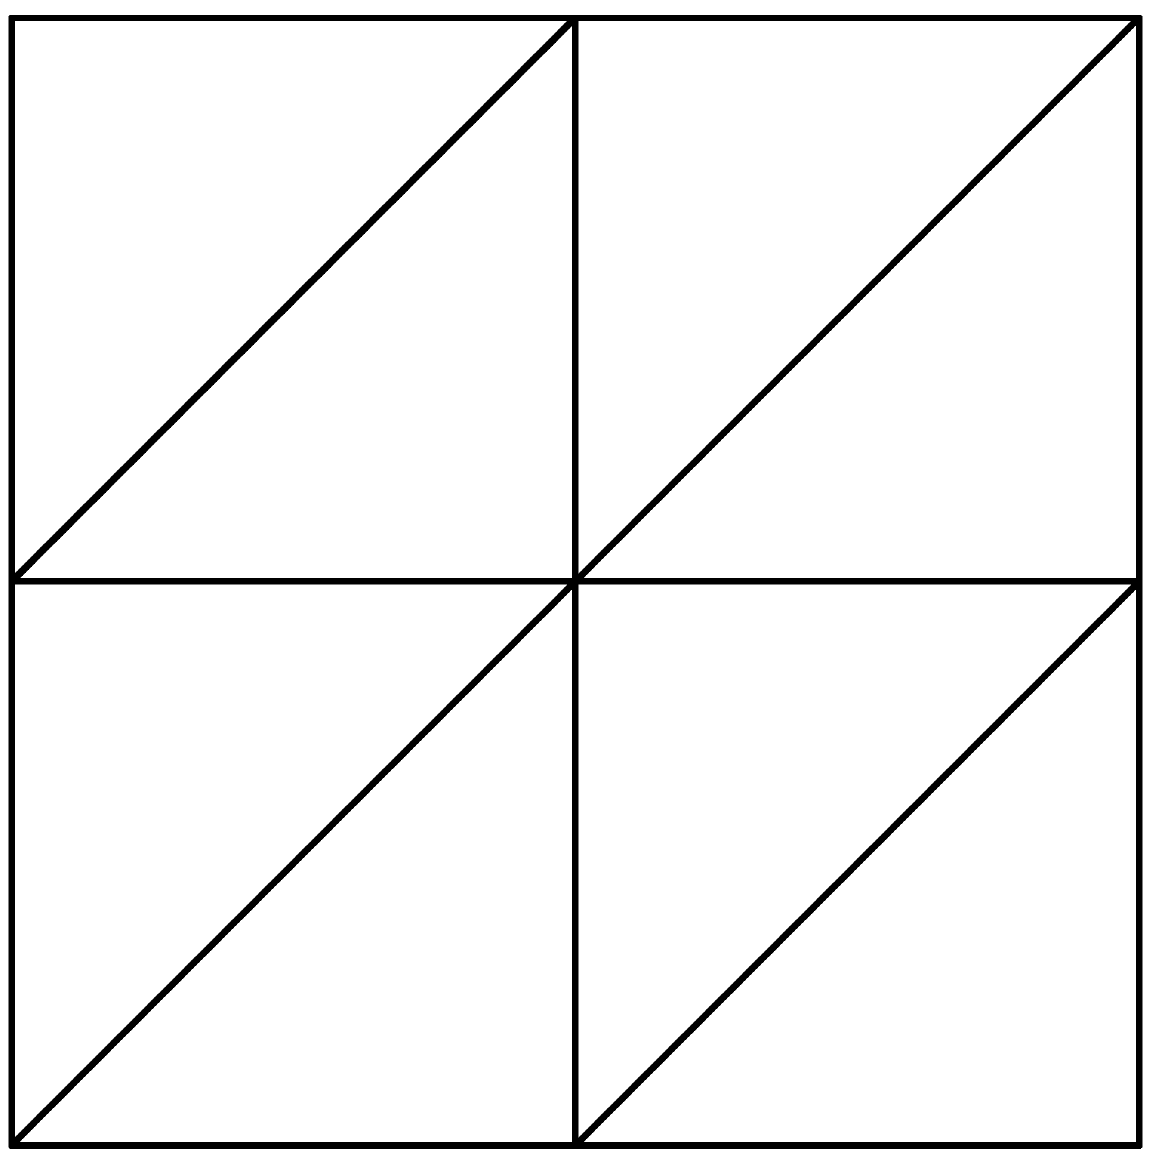
\includegraphics[width=0.15\textwidth]{grid.png} 
	\end{center}
	$$ 
\hskip0.05 in \mathcal T_1\hskip 0.7in \mathcal T_2\hskip 0.7in  \mathcal T_3\hskip 0.7in \mathcal T_4
	$$
	\caption{multilevel grids for piecewise linear functions}
\end{figure}




The grid points of these grids can be given by
$$
x_i^{\ell}=i h_{\ell}, y_j^{\ell}=j h_{\ell},  i=0, \ldots, m_\ell-1,
j=0, \ldots, n_\ell-1.
$$
Here $h_{\ell} = 2^{-s + \ell -1}a$ for some $a >0$. The above geometric coordinates $(x_i^\ell, y_j^\ell)$
are usually not used in image precess literatures, but they are relevant
in the context of multigrid method for numerical solution of PDEs.
We now consider piecewise bilinear (or linear) functions on the sequence of grids
\eqref{grids} and we obtain a nested sequence of linear vector spaces
\begin{equation}
\label{Vk}
\mathcal V_1\supset\mathcal V_2\supset\ldots\supset \mathcal
V_J.
\end{equation}





\begin{figure} \label{mugrid-bi}
\begin{center}
\setlength{\unitlength}{0.445mm}
\begin{picture}(45,45)(50,0)
\linethickness{0.1mm}
\multiput(-20,0)(2.5,0){17}{\line(0,1){40}}
\multiput(-20,0)(0,2.5){17}{\line(1,0){40}}
\multiput(28,0)(5,0){9}{\line(0,1){40}}
\multiput(28,0)(0,5){9}{\line(1,0){40}}
\multiput(77,0)(10,0){5}{\line(0,1){40}}
\multiput(77,0)(0,10){5}{\line(1,0){40}}
\multiput(126,0)(20,0){3}{\line(0,1){40}}
\multiput(126,0)(0,20){3}{\line(1,0){40}}
\end{picture}
\setlength{\unitlength}{0.5mm}
\end{center}
$$ 
\hskip0.05 in \mathcal T_1\hskip 0.7in \mathcal T_2\hskip 0.7in  \mathcal T_3\hskip 0.7in \mathcal T_4
$$
\caption{multilevel grids for piecewise bilinear functions}
\end{figure}
%\subsection{Nodal bases and dual bases on multilevel spaces}
%\noindent\textbf{Nodal bases and dual bases on multilevel spaces}

Here each $\mathcal V_\ell$ consists of all piecewise linear (or bilinear)
functions with respect to the grid \eqref{grids} and \eqref{mn-ell}.
Each $\mathcal V_\ell $ has a set of basis functions:
$\phi_{i,j}^\ell\in \mathcal V_\ell$ satisfying:
\begin{equation}
\label{NodalBases-mul}
\mathbf\phi_{i,j}^\ell(x_p^\ell,y_q^\ell)=\delta_{(i,j), (p,q)} = 
\begin{cases}
1 \quad &\text{if} \quad (p,q) = (i,j), \\
0 \quad &{\text{if}} \quad (p,q)\neq (i,j).
\end{cases}
\end{equation}
\begin{figure}[!ht]
\begin{center}
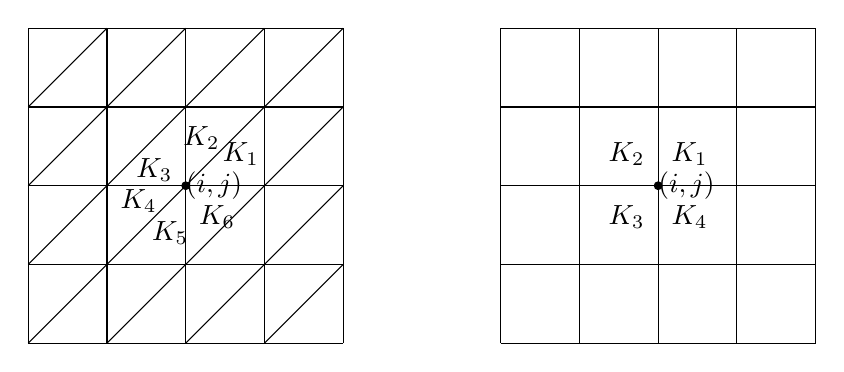
\begin{tikzpicture}[xscale=2,yscale=2]
%\tikzstyle{every node}=[font=\Large,scale=0.9]
\draw[-] (0,0) -- (2,0);
\draw[-] (0,0.5) -- (2,0.5);
\draw[-] (0,1) -- (2,1);
\draw[-] (0,1.5) -- (2,1.5);
\draw[-] (0,2) -- (2,2);

\draw[-] (0,0) -- (0,2);
\draw[-] (0.5,0) -- (0.5,2);
\draw[-] (1,0) -- (1,2);
\draw[-] (1.5,0) -- (1.5,2);
\draw[-] (2,0) -- (2,2);

\draw[-] (0,0) -- (2,2);
\draw[-] (0,0.5) -- (1.5,2);
\draw[-] (0,1) -- (1,2);
\draw[-] (0,1.5) -- (0.5,2);
\draw[-] (0.5,0) -- (2,1.5);
\draw[-] (1,0) -- (2,1);
\draw[-] (1.5,0) -- (2,0.5);

\node at (1.35,1.2) {$K_1$};
\node at (1.1,1.3) {$K_2$};
\node at (0.8,1.1) {$K_3$};
\node at (0.7,0.9) {$K_4$};
\node at (0.9,0.7) {$K_5$};
\node at (1.2,0.8) {$K_6$};

\node at (1.18, 1) {$(i,j)$};

\fill(1,1) circle(0.8pt);

\draw[-] (3,0) -- (5,0);
\draw[-] (3,0.5) -- (5,0.5);
\draw[-] (3,1) -- (5,1);
\draw[-] (3,1.5) -- (5,1.5);
\draw[-] (3,2) -- (5,2);

\draw[-] (3,0) -- (3,2);
\draw[-] (3.5,0) -- (3.5,2);
\draw[-] (4,0) -- (4,2);
\draw[-] (4.5,0) -- (4.5,2);
\draw[-] (5,0) -- (5,2);

\node at (4.2,1.2) {$K_1$};
\node at (3.8,1.2) {$K_2$};
\node at (3.8,0.8) {$K_3$};
\node at (4.2,0.8) {$K_4$};
\node at (4.18,1) {$(i,j)$};
\fill(4,1) circle(0.8pt);
\end{tikzpicture}
\end{center}
\end{figure}

For the piecewise linear finite element space, the nodal basis function $\phi^\ell_{i,j}$  associate with each $(x_i^\ell,y_j^\ell)$   
(satisfying \eqref{NodalBases-mul}) is given by 
\begin{equation}
  \label{LinearNodalBasis}
  \phi_{i,j}^\ell(x,y)=\left\{
  \begin{array}{ll}
\frac{x^\ell_{i+1}-x}{h}, & (x,y)\in K_1, \\
\frac{y^\ell_{j+1}-y}{h}, &(x,y)\in K_2,\\
\frac{x-x^\ell_{i-1}-(y-y^\ell_j)}{h}, &(x,y)\in K_3,\\
\frac{x-x^\ell_{i-1}}{h}, &(x,y)\in K_4,\\
\frac{y-y^\ell_{j-1}}{h}, &(x,y)\in K_5,\\
\frac{x^\ell_{i+1}-x+y-y^\ell_j}{h}, &(x,y)\in K_6\\
0, & \mbox{ elsewhere.} 
\end{array}
\right.
\end{equation}
shown in Fig. \ref{fig:nodallinear}.
\begin{figure}
\centering
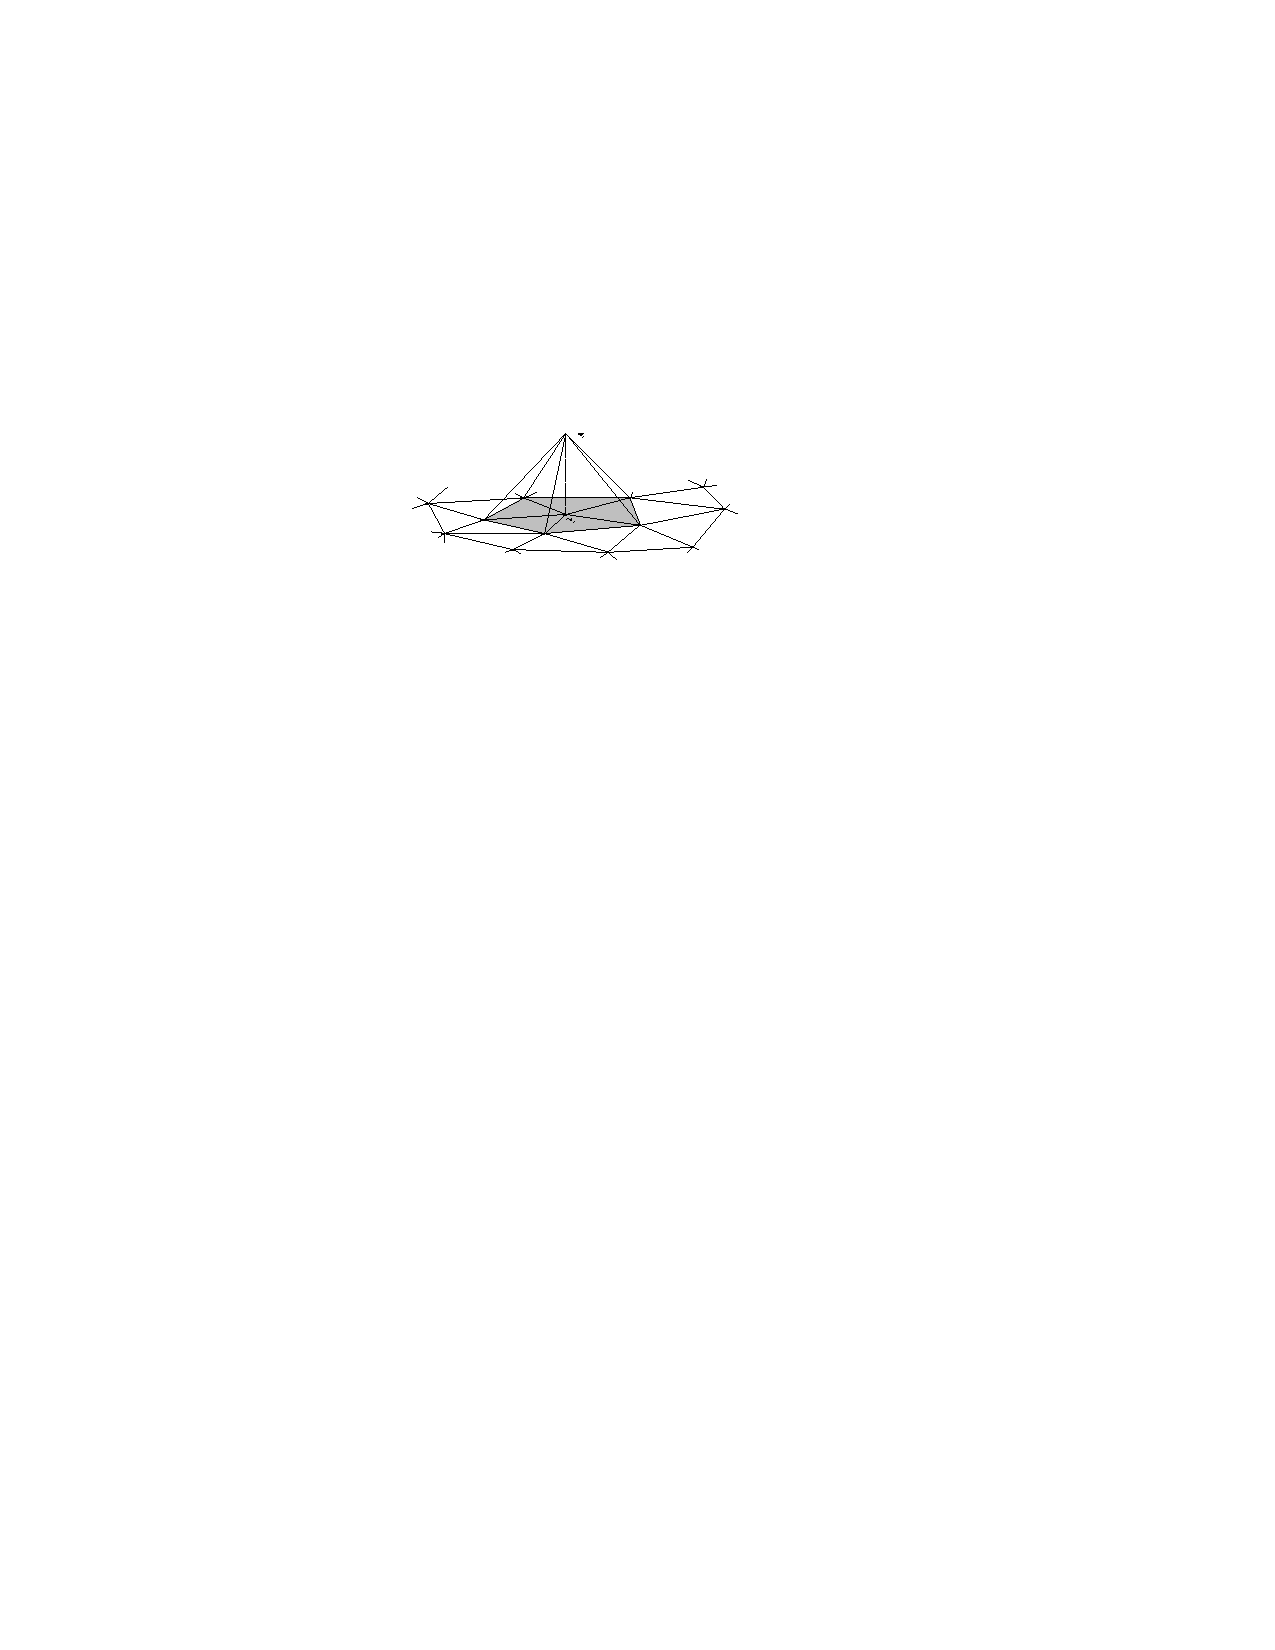
\includegraphics[width=5.5cm,height=5cm]{figures/nodalbasis.pdf} 
\caption{\footnotesize{Nodal basis for linear element.}}
\label{fig:nodallinear}
\end{figure}

For bilinear element, it is easy to see that the nodal basis function $\phi^\ell_{i,j}$  associated with each $(x^\ell_i,y^\ell_j)$   
(satisfying \eqref{NodalBases-mul}) is given by 
\begin{equation}
  \label{BilinearNodalBasis}
  \phi^\ell_{i,j}(x,y)=\left\{
  \begin{array}{ll}
\frac{(x^\ell_{i+1}-x)(y^\ell_{j+1}-y)}{h^2}, \quad& (x,y)\in K_1, \\
\frac{(x-x^\ell_{i-1})(y^\ell_{j+1}-y)}{h^2}, \quad &(x,y)\in K_2,\\
\frac{(x-x^\ell_{i-1})(y-y^\ell_{j-1})}{h^2},\quad &(x,y)\in K_3,\\
\frac{(x^\ell_{i+1}-x)(y-y^\ell_{j-1})}{h^2},\quad &(x,y)\in K_4,\\
0 \quad & \mbox{ elsewhere.} 
\end{array}
\right.
\end{equation}


Associated with the above nodal basis functions $\phi^{\ell}_{i,j}(x,y)\subset \mathcal V_{\ell}$, 
we define the corresponding dual basis functions $\psi^{\ell}_{i,j}(x,y)\subset \mathcal V_{\ell}$ 
satisfying 
\begin{equation}
  \label{dual-basis}
(\psi^{\ell}_{i,j}(x,y), \phi^{\ell}_{p,q}(x,y))_{L^2(\Omega)}=\delta_{(i,j), (p,q)}.
\end{equation}
The existence of dual basis functions is obvious, but the exact expression of the dual basis functions are  
in general difficult to obtain. In fact, \eqref{dual-basis} is the only property that is needed in the application 
of dual basis. 

We write $\mathbf u_h(x,y)=\sum\limits_{i,j=1}^{n} u_{i,j}\phi_{i,j}(x,y), \mathbf v_h(x,y)=\sum\limits_{i,j=1}^{n} v_{i,j}\phi_{i,j}(x,y)$. 

\begin{lemma}
For bilinear functions, we have  
\begin{equation}\label{basis:plongation}
\begin{split}
\phi_{i,j}^{\ell+1}(x,y)&=\phi_{2i,2j}^{\ell}(x,y)+\frac{1}{2}\left(\phi_{2i-1,2j}^{\ell}(x,y)+\phi_{2i,2j-1}^{\ell}(x,y)
+\phi_{2i+1,2j}^{\ell}(x,y)+\phi_{2i,2j+1}^{\ell}(x,y)\right)\\
&+\frac{1}{4}\left(\phi_{2i-1,2j-1}^{\ell}(x,y)+\phi_{2i+1,2j-1}^{\ell}(x,y)
+\phi_{2i+1,2j+1}^{\ell}(x,y)+\phi_{2i-1,2j+1}^{\ell}(x,y)\right).
\end{split}
\end{equation}
For linear functions, we have  
\begin{equation}\label{basis:plongation2}
\begin{split}
\phi_{i,j}^{\ell+1}(x,y)&=\phi_{2i,2j}^{\ell}(x,y)
+\frac{1}{2}\left(\phi_{2i-1,2j-1}^{\ell}(x,y)+\phi_{2i+1,2j+1}^{\ell}(x,y)\right)\\
&+\frac{1}{2}\left(\phi_{2i-1,2j}^{\ell}(x,y)+\phi_{2i,2j-1}^{\ell}(x,y)
+\phi_{2i+1,2j}^{\ell}(x,y)+\phi_{2i,2j+1}^{\ell}(x,y)\right).
\end{split}
\end{equation}
\end{lemma}
Thus, for each $\mathbf v^{\boldsymbol {\ell}} \in \mathcal V_{\ell}, \mathbf f^{\boldsymbol {\ell}} \in \mathcal V'_{\ell}=\mathcal V_{\ell}$, we have 
\begin{equation}\label{expand}
\mathbf v^{\boldsymbol \ell}(x,y)=\sum_{i=1}^{m_\ell}\sum_{j=1}^{n_\ell}v^\ell_{i,j}\phi_{i,j}^\ell(x,y), 
~~ \mathbf f^{\boldsymbol \ell}(x,y)=\sum_{i=1}^{m_\ell}\sum_{j=1}^{n_\ell}f^\ell_{i,j}\psi_{i,j}^\ell(x,y),
\end{equation}
where
\begin{equation}
  \label{vf}
  v^\ell_{i,j}=\mathbf v^\ell(x_i^\ell,y_j^\ell),~~ f_{i,j}^\ell= (\mathbf f^\ell, \phi^\ell_{i,j})_{L^2(\Omega)}.
\end{equation}
Let us introduce the following tensors: 
\begin{equation}
  \label{v}
  v^\ell=(v^\ell_{i,j}),~~f^\ell=(f^\ell_{i,j}),~~\phi^\ell=(\phi^\ell_{i,j}),~~\psi^\ell=(\psi^\ell_{i,j}).
\end{equation}
The following identities obviously hold: 
$$
\mathbf v^\ell=(v^\ell, \phi^\ell)_{l^2},~~\mathbf f^\ell=(f^\ell, \psi^\ell)_{l^2},~~(\mathbf f^\ell,\mathbf v^\ell)_{L^2(\Omega)}=(f^\ell, v^\ell)_{l^2}.
$$


%\newcommand{\fix}{\marginpar{FIX}}
%\newcommand{\new}{\marginpar{NEW}}
%\newcommand{\classmap}{H}
%\newcommand{\linearize}{H_0}
%\newcommand{\linear}{L}
%\newcommand{\FC}{{\mathcal D}}
%\example
Denote $\phi^{\ell}=(\phi^{\ell}_{i,j})\in \mathbb R^{m_{\ell}\times n_{\ell}}$, 
by the definitions of convolution \eqref{con1} and stride \eqref{stride}, \eqref{basis:plongation} means that
$$
 \phi^{\ell+1}=R\ast_2 \phi^{{\ell}},
$$
where 
\begin{equation}\label{bi-restrict}
R=
%\left\{
\begin{cases}
	\begin{pmatrix}
	\frac{1}{4} &\frac{1}{2}&\frac{1}{4}\\
	\frac{1}{2}& 1&\frac{1}{2}\\
	\frac{1}{4}&\frac{1}{2}&  \frac{1}{4} 
	\end{pmatrix}
	\hbox{~~for bilinear functions};\\
	\begin{pmatrix}
	0 &\frac{1}{2}&\frac{1}{2}\\
	\frac{1}{2}& 1&\frac{1}{2}\\
	\frac{1}{2}&\frac{1}{2}&  0
	\end{pmatrix}
	\hbox{~~for linear functions}.
	\end{cases}
	%\right.
	\end{equation}		
\section{Deconvolution}
For any linear mapping $\mathcal C: \mathbb{R}^{m\times n} \mapsto \mathbb{R}^{m'\times n'}$, 
its transpose is the unique linear mapping $\mathcal C^\top: \mathbb{R}^{m'\times n'} \mapsto \mathbb{R}^{m\times n}$
satisfying 
$$
(\mathcal C^\top u, v)_{l^2}=(u, \mathcal C v)_{l^2}~~~\forall~u\in \mathbb{R}^{m'\times n'} , v\in \mathbb{R}^{m\times n}
$$
Associated with any kernel $K$, a deconvolution is defined as the transpose of convolution 
with stride $2$ with respect to the $l^2$-inner product as:
\begin{equation}\label{eq:def_deconv}
 (u, K \ast_2^\top v)_{l^2}=(K \ast_2 u, v)_{l^2},
\end{equation}
with
\begin{equation}
u \in \mathbb{R}^{m \times n} \quad \text{and} \quad v \in \mathbb{R}^{\frac{m+1}{2} \times \frac{m+1}{2}}.
\end{equation}

\begin{lemma}\label{lemm:tilde-K}
For any $K \in \mathbb{R}^{(2k+1) \times (2k+1)}$,
\begin{equation}\label{eq:}
K\ast_2^\top = {\tilde K}\ast \mathcal S^\top,
\end{equation}
where $\tilde K$ is defined as
\begin{equation}\label{eq:def_tildeK}
\tilde K_{p,q} = K_{-p, -q}, \quad p,q = -k:k.
\end{equation}
Intuitively, if we take $K_{0,0}$ as the center for the convolutional kernel $K$, 
then $\tilde K$ is the central symmetry of $K$. 
In 2D case, it can also be understood as the rotation of $\pi$ with respect to
the center $K_{0,0}$.
\end{lemma}

Recalling the definition of deconvolution in \eqref{eq:def_deconv}, we have
\begin{equation}\label{eq:op_deconv}
\begin{aligned}
(u,  K \ast_2^\top v)_{l^2} &= (K \ast_2 u, v)_{l^2} = (\mathcal S \mathcal C_K u, v)_{l^2} \\
&= (u,  \mathcal C^\top_K \mathcal S^\top v)_{l^2},
\end{aligned}
\end{equation}
with definition
\begin{equation}\label{eq:de_stride_dim}
\mathcal S^\top:   \mathbb{R}^{\frac{m+1}{2} \times\frac{n+1}{2}} \mapsto \mathbb{R}^{m\times n},
\end{equation}
and 
\begin{equation}\label{eq:de_stride}
[\mathcal S^\top (f)]_{i,j} = 
\begin{cases}
0 \quad &\text{if i or j is even}, \\
f_{i/2, j/2}, \quad &\text{else}.
\end{cases}
\end{equation}

Thus to say, we have the simple version of the deconvolution for $K \ast $ as
\begin{equation}\label{eq:simple_deconv}
K \ast_2^\top v = \mathcal C_K^\top \circ \mathcal S^\top (v) = \mathcal C_{\tilde K} \circ \mathcal S^\top (v) = \tilde K \ast \mathcal S^\top (v),
\end{equation}
thus to say
\begin{equation}\label{eq:final}
K \ast_2^\top  = \tilde K \ast \mathcal S^\top.
\end{equation}

In short, we have the next decomposition
\begin{itemize}
	\item convolution with stride = stride $ \circ$ convolution,
	\item deconvolution with stride  = transposed convolution $\circ$ transposed stride = convolution with the central symmetry of original kernel $\circ$ transposed stride.
\end{itemize}

\begin{theorem}\label{thm:deconv_op}

Let us consider 
\begin{equation}
K=(K_{p,q}),~~p,q = -1, 0, 1.
\end{equation}
Then we have 
$$
K \ast_2^\top v = \tilde K \ast \mathcal S^\top (v).
$$
As in \eqref{eq:de_stride} and the Lemma \ref{lemm:tilde-K}, we have the 
final version is 
\begin{equation}
\label{eq:7}
[K \ast_2^\top v ]_{2i,2j}=  K_{0,0}v_{i,j},
\end{equation}
with 
\begin{equation}
\label{eq:9}
[K \ast_2^\top v ]_{2i-1, 2j} = K_{0,1}v_{i-1,j} + K_{0,-1}v_{i,j}, \quad 
[K \ast_2^\top v ]_{2i, 2j-1} = K_{1,0}v_{i,j} + K_{-1,0}v_{i,j-1},
\end{equation}
and
\begin{equation}
%\begin{tiny}
%{\scriptsize 
[K \ast_2^\top v ]_{2i-1, 2j-1}  =  
K_{1,1}v_{i,j} + K_{-1,1}v_{i-1,j} + K_{1,-1}v_{i,j-1} + K_{-1,-1}v_{i-1,j-1}.
%\end{tiny}
%}
\end{equation}
\end{theorem}
\begin{remark}
Deconvolution can obviously be also defined for general stride $s$, but we believe it is sufficient to use $s=2$
in most applications. 
\end{remark}

 
\section{Linear feature mappings}
We consider the following linear mapping
\begin{equation}
  \label{feature-map}
\mathbf A\mathbf u=\mathbf  f  
\end{equation}
where 
\begin{equation}
  \label{map-A}
\mathbf A: \mathcal V\mapsto \mathcal V'.
\end{equation}
For example, for the elliptic problem \eqref{laplace}, $(\mathbf A \mathbf u, \mathbf v)=(\nabla u_h, \nabla v_h)$.
We consider the restriction of the mapping $\mathbf A_1\equiv \mathbf A$ on the coarser multilevel spaces:
\begin{equation}
  \label{map-A-ell}
\mathbf A_{\ell}: \mathcal V_\ell\mapsto \mathcal V'_\ell
\end{equation}
and the corresponding equation read as:
\begin{equation}
  \label{feature-map-ell}
\mathbf A_\ell \mathbf u^\ell=\mathbf f^\ell.
\end{equation}
In image process, we can view $\mathbf f$ as the input images and $\mathbf u$ as the extracted features of the original image $\mathbf f$.  We then view $\mathbf f^\ell$ as the projection of images on a coarser resolution and $\mathbf u^\ell$ as the extracted features of the coarsened image $\mathbf f^\ell$.

One main question is how to obtain coarser images and features defined by \eqref{feature-map-ell} from the original equation \eqref{feature-map}.  We now consider a special technique.

We define $\mathbf u^\ell\in \mathcal V_\ell$ by
\begin{equation}
  \label{u_ell}
(\mathbf A\mathbf u^\ell,\mathbf v^\ell)=  (\mathbf f,\mathbf v^\ell), \quad\forall \mathbf v^\ell\in\mathcal V_\ell
\end{equation}
\begin{lemma}
The restricted $\mathbf u^\ell\in\mathcal V_\ell$ defined by \eqref{u_ell} satisfies \eqref{feature-map-ell} if 
$\mathbf A_\ell: \mathcal V_\ell\mapsto \mathcal V_\ell'$ and $\mathbf f_\ell\in \mathcal V_\ell'$ are defined by
\begin{equation}
  \label{A-ell}
(\mathbf A_\ell \mathbf u^\ell,\mathbf v^\ell)=  (\mathbf A\mathbf u^\ell,\mathbf v^\ell), \quad\forall \mathbf v^\ell\in\mathcal V_\ell
\end{equation}
\begin{equation}
  \label{u-ell}
(\mathbf f^\ell,\mathbf v^\ell)=  (\mathbf f,\mathbf v^\ell), \quad\forall \mathbf v^\ell\in\mathcal V_\ell
\end{equation}
\end{lemma}


\section{Restriction and prolongation under the convolution notation}
Now we derive the restriction and prolongation as follows. We show the details for the case of bilinear functions here. The 
case of linear function can be shown similarly. 
Let $f_{i,j}^{\ell+1}=(\mathbf f^\ell,\phi^{\ell+1}_{i,j})_{L^2(\Omega)}$, then we have
\begin{equation}
\begin{split}
  f^{\ell+1}&=\int_{\Omega} \mathbf f^\ell \phi^{\ell+1}=\sum\limits_{i=1}^{m_\ell}\sum\limits_{j=1}^{n_\ell}
 \int_{\Omega}f_{i,j}^{\ell}\psi_{i,j}^\ell\left[(R\ast_2) \phi^\ell\right]
=\sum\limits_{i=1}^{m_\ell}\sum\limits_{j=1}^{n_\ell} f_{i,j}^{\ell}(R\ast_2)\int_{\Omega}\psi_{i,j}^\ell \phi^\ell\\
&=\sum\limits_{i=1}^{m_\ell}\sum\limits_{j=1}^{n_\ell}(R\ast_2)f_{i,j}^{\ell}e_ie_j^T=R\ast_2 f^{\ell}.
\end{split}
\end{equation}
Hence the restriction 
$$
R^{\ell+1}_\ell: \mathbb R^{m_{\ell}\times n_{\ell}}\mapsto  \mathbb R^{m_{\ell+1}\times n_{\ell+1}} 
$$
is obtain by $R^{\ell+1}_\ell  f^{\ell}= R\ast_2  f^{\ell}$ with $R\in \mathbb R^{3\times 3}$ given by  \eqref{bi-restrict}, namely
\begin{equation}\label{restriction:freedom}
\begin{split}
f_{i,j}^{\ell+1}&=f^{\ell}_{2i,2j}+\frac{1}{2}(f^{\ell}_{2i-1,2j}+f^{\ell}_{2i,2j-1}+f^{\ell}_{2i+1,2j}+f^{\ell}_{2i,2j+1})\\
&+\frac{1}{4}\left(f^{\ell}_{2i-1,2j-1}+f^{\ell}_{2i+1,2j-1}+f^{\ell}_{2i+1,2j+1}+f^{\ell}_{2i-1,2j+1}\right).
\end{split}
\end{equation}

Next 
let $\mathbf u^{\ell+1}=\sum\limits_{i=1}^{m_{\ell+1}}\sum\limits_{j=1}^{n_{\ell+1}}u_{i,j}^{\ell+1}\phi^{\ell+1}_{i,j}
=( \mathbf u^{\ell+1}, \phi^{\ell+1})_{l^2}$, then we have
\begin{equation}
\begin{split}
\mathbf u^{\ell+1}&=( u^{\ell+1}, \phi^{\ell+1})_{l^2}
=( u^{\ell+1}, R\ast_2\phi^{\ell})_{l^2}=(R\ast_2^{\top} u^{\ell+1}, \phi^{\ell})_{l^2}\\
&=\sum\limits_{i=1}^{m_{\ell}}\sum\limits_{j=1}^{n_{\ell}}\left(R\ast_2^{\top} u^{\ell+1}\right)_{i,j}\phi^{\ell}_{i,j}.
\end{split}
\end{equation}
Namely
$$
\mathbf u^{\ell+1}(x_i^\ell,y_j^\ell)=\left(R\ast_2^{\top} u^{\ell+1}\right)_{i,j}.
$$
And we obtain the prolongation 
$$
P_{\ell+1}^\ell=R\ast_2^{\top} : \mathbb R^{m_{\ell+1}\times n_{\ell+1}}\mapsto  \mathbb R^{m_{\ell}\times n_{\ell} }
$$
is defined by 
$$
u^\ell_{2i,2j}=u^{\ell+1}_{i,j},
$$
$$
u^\ell_{2i-1,2j}=\frac{1}{2}(u^\ell_{i,j}+u^\ell_{i-1,j}),~~~ u^\ell_{2i,2j-1}=\frac{1}{2}(u^{\ell+1}_{i,j}+u^{\ell+1}_{i,j-1})
$$
and 
$$
u^\ell_{2i-1,2j-1}=\frac{1}{4}(u^{\ell+1}_{i,j}+u^{\ell+1}_{i-1,j}+u^{\ell+1}_{i-1,j-1}+u^{\ell+1}_{i,j-1}).
$$
In summery, we have the restriction and prolongation as follows: 
\begin{lemma}\label{ris:plon}
The restriction 
$$
R^{\ell+1}_\ell: \mathbb R^{m_\ell\times n_\ell}\mapsto  \mathbb R^{m_{\ell+1}\times n_{\ell+1}}~~\hbox{is}~~ R^{\ell+1}_\ell = R\ast_2  
$$ 
and the prolongation
$$
P_{\ell+1}^{\ell}: \mathbb R^{m_{\ell+1}\times n_{\ell+1}}\mapsto  \mathbb R^{m_{\ell}\times n_{\ell} } ~~\hbox{is}~~ P^{\ell}_{\ell+1} =R\ast_2^{\top} 
$$
where 
\begin{equation}\label{bi-restrict1}
R=
%\left\{
\begin{cases}
	\begin{pmatrix}
	\frac{1}{4} &\frac{1}{2}&\frac{1}{4}\\
	\frac{1}{2}& 1&\frac{1}{2}\\
	\frac{1}{4}&\frac{1}{2}&  \frac{1}{4} 
	\end{pmatrix}
	\hbox{~~for bilinear functions};\\
	\begin{pmatrix}
	0 &\frac{1}{2}&\frac{1}{2}\\
	\frac{1}{2}& 1&\frac{1}{2}\\
	\frac{1}{2}&\frac{1}{2}&  0
	\end{pmatrix}
	\hbox{~~for linear functions}.
	\end{cases}
	%\right.
	\end{equation}	
\end{lemma}

Let $(\phi^{\ell}_{i,j})$ is a basis of $\mathcal V_\ell$, for any $\mathbf u^\ell \in \mathcal V_\ell$, then $\mathbf u^{\ell}=\sum\limits_{i=1}^{m_{\ell}}\sum\limits_{j=1}^{n_{\ell}}u_{i,j}^{\ell}\phi^{\ell}_{i,j}$, and we denote $u^\ell=(u_{i,j}^{\ell})\in  \mathbb R^{m_{\ell}\times n_{\ell} }$ the matrix representation of $\mathbf u^\ell$ under the basis $(\phi^{\ell}_{i,j})$.
Let $(\psi^{\ell}_{s,t})$ is a basis of $\mathcal V'_\ell$ which is dual to $(\phi^{\ell}_{i,j})$. Denote $A_\ell=(a_{stij}^{\ell})$ the tensor representation of $\mathbf A_\ell: \mathcal V_\ell\mapsto \mathcal V'_\ell $ and defined as 
$$
\mathbf A_\ell \phi^\ell_{i,j}=\sum\limits_{s=1}^{m_{\ell}}\sum\limits_{t=1}^{n_{\ell}}a_{stij}^{\ell}\psi^\ell_{s,t}.
$$
Hence $a_{stij}^{\ell}=(\mathbf A_\ell \phi^\ell_{i,j}, \phi^\ell_{s,t})$. From $(\mathbf A_{\ell+1}\phi^{\ell+1}_{i,j}, \phi^{\ell+1}_{s,t})=(\mathbf A_\ell\phi^{\ell+1}_{i,j}, \phi^{\ell+1}_{s,t})$, we have
$$
a_{stij}^{\ell+1}=\sum_{r=1}^{m_\ell}\sum_{q=1}^{n_\ell}\left(\sum_{k=1}^{m_\ell}\sum_{m=1}^{n_\ell} P_{kmij}^{\ell,{\ell+1}} a_{rqkm}^\ell\right)P_{rqst}^{\ell,{\ell+1}} 
$$ 
Where $P^{\ell,{\ell+1}}=(P_{rqst}^{\ell,{\ell+1}})$ is the tensor representation of the prolongation $P_{\ell+1}^{\ell}$.


Consider the finite element method on two different grids 
$\mathcal T_\ell,~\mathcal T_{\ell+1},~h_{\ell+1}=2h_\ell, \mathcal V_{\ell+1}\subset \mathcal V_{\ell}$. 
With the restriction $R_{\ell}^{\ell+1}$ and prolongation $P_{\ell+1}^\ell$ obtained in Lemma \ref{ris:plon}, we have the following relationship to define coarse operation
\begin{equation}\label{eq:def_coarse}
\begin{aligned}
 A_{\ell+1}&=R_{\ell}^{\ell+1}  A_{\ell}P_{\ell+1}^{\ell}.  \\
&= R \ast_2 A_\ell \ast (R\ast_2^\top),   \quad (\ell = 1:J-1),
\end{aligned}
\end{equation}
with $A_1 = A$. 
\begin{theorem}
If $R$ is consistent with $A_\ell$ which means that $R$ should be linear or bi-linear as $A_\ell$, then we have
the $A_{\ell+1}$ operation in coarse grid defined in \eqref{eq:def_coarse} is the same with $A_\ell$.
\end{theorem}
\begin{proof}
For any $u_{\ell+1}$ and $v_{\ell+1}$ in $\mathcal V_{\ell+1}$, it remains to prove that
$$
(A_\ell P_{\ell+1}^\ell u_{\ell+1},P_{\ell+1}^\ell v_{\ell+1}) = (A_{\ell+1}u_{\ell+1}, v_{\ell+1})
$$
where $A_\ell$ and $A_{\ell+1}$ are the tensor representation of $\mathbf A_\ell$ and $\mathbf A_{\ell+1}$.

We can also view them as convolutions. By the definition of operators $R_{\ell}^{\ell+1}$ and $P_{\ell+1}^\ell$, a direct computation gives the above result.
\end{proof}
\begin{proof}
By the definition above, we have that
\begin{equation}
A_{\ell+1} (v) = \mathcal S\left( (R\ast A_{\ell} \ast R )\ast \mathcal S^\top(v) \right),
\end{equation}
because of the properties of convolution we know that 
\begin{equation}\label{eq:K=RAR}
(R\ast A_{\ell} \ast R )\ast = K \ast,
\end{equation}
for some 
$$
K \in \mathbb{R}^{7\times 7}.
$$
Then we have the next computation for $A_{\ell+1}(v)$
\begin{equation}\label{eq:compute_A}
\begin{aligned}
[A_{\ell+1} (v)]_{i,j} &= [\mathcal S\left( (R\ast A_{\ell} \ast R )\ast \mathcal S^\top(v) \right)]_{i,j}, \\
&= [ K\ast  \mathcal S^\top(v)]_{2i,2j}, \\
&= \sum_{p,q=-3}^{3} [\mathcal S^\top (v)]_{2i+p, 2j+q} K_{p,q}, \\
&= \sum_{p,q=-1}^1  [\mathcal S^\top (v)]_{2(i+p), 2(j+q)} K_{2p,2q}, \\
&= \sum_{p,q=-1}^1  v_{i+p, j+q} \hat K_{p,q}, \\
\end{aligned}
\end{equation}
	
Thus to say, we have
\begin{equation}
A_{\ell+1}(v) =  \hat K \ast v,
\end{equation}
with 
$$
\hat K_{p,q} = K_{2p,2q}, \quad p,q = -1,0,1,
$$
with $K$ is defined in \eqref{eq:K=RAR}.

Then by the direct computation of \eqref{eq:K=RAR} as 
$$
(R\ast A_{\ell} \ast R )\ast = K \ast
$$
and take the even index we have that
\begin{equation}
A_{\ell+1} = \hat K = A_\ell,
\end{equation}
if $R$ is consistent with $A_\ell$ which means that $R$ should be linear or bi-linear as $A_\ell$.	
\end{proof}



\section{Multigrid for finite element methods}
By the definition of convolution \eqref{con1}, we can rewrite \eqref{2d-fe0} and \eqref{2d-fe1} as follows: 
\begin{equation}\label{conA}
A\ast:  \mathbb{R}^{m\times n}\rightarrow \mathbb{R}^{m\times n},~~~A\ast u=f,~~\Leftrightarrow~~ u=\argmin J(v)=\argmin \left(\frac{1}{2}(A\ast v,v)-(f,v)_{l^2}\right)
\end{equation}
where $u=(u_{ij})$, $f=(f_{ij})$, 
\begin{equation}\label{fe0_Ka}
A=\left\{
\begin{array}{ll}
	\begin{pmatrix}
	0 &-1&0\\
	-1& 4&-1\\
	0 &-1& 0
	\end{pmatrix}
&\text{for linear finite element,}	\\
%	\begin{equation}\label{fe1_Ka}
%	K_A=
	\begin{pmatrix}
	-1 &-1&-1\\
	-1& 8&-1\\
	-1 &-1& -1
	\end{pmatrix}
&\text{for bilinear finite element.}
\end{array}\right.
	\end{equation}

It is easy to see that 
$$
\nabla J(v)= A\ast v - f := - r,\quad r=f-A\ast v.
$$
Applying the gradient descent method to \eqref{minProblem}, we obtain the following iterative method: 
\begin{equation}\label{iterativeAst}
u^{k+1} = u^k + \eta r^k,\quad r^k = f-A\ast u^k.
\end{equation}
Here we can clearly see that gradient descent method is equivalent to
damped Jacobi method. Usually, we call this as smoother. 
\begin{lemma}
The gradient descent method \eqref{iterativeAst} for linear finite element converges if $\eta={1\over 8} %\in (0,1/4)
$, and the one for bilinear finite element converges  if $\eta={1\over 16}% \in (0,1/8)
$. Furthermore, the high frequence in $u-u^k$ are damped very rapidly. 
\end{lemma}
\begin{proof}
According to \eqref{iterativeAst} ,
$$
u^{k+1}-u=(I-\eta A)\ast (u^k-u).
$$
The gradient descent method \eqref{iterativeAst} converges if $\rho((I-\eta A)\ast)<1$, namely $\eta\rho(A\ast)<2$. For linear finite element, if $\eta= {1\over 8}$, $\rho(A\ast )<8$, thus the gradient descent method \eqref{iterativeAst} converges.
For bilinear finite element, if $\eta= {1\over 16}$, $\rho(A\ast )<16$, thus the gradient descent method \eqref{iterativeAst} converges.

For linear finite element, let $(\lambda_i, v_i)$ satisfy $A\ast v_i=\lambda_i v_i$ and $0<\lambda_1\leq \lambda_2\leq\cdots\lambda_{N}$ with $N=n^2$. Expand the error $u^k-u$ in terms of eigenvectors $v_i$, namely,
$$
u^k-u=\sum_{i=1}^{N} a_i^kv_i.
$$
Then
$$
u^{k}-u=\sum_{i=1}^{N} a_i^k(1-\eta \lambda_i)v_i=\sum_{i=1}^{N} a_i^0(1-\eta \lambda_i)^{k}v_i.
$$
According to Proposition \ref{prop:A}, it is easy to see that 
$$
1-{1\over 8}\lambda_N\approx {\pi^2\over 4(n+1)^2} \ll 1.
$$
For $\eta={1\over 8}$, the coefficient $a_N^0(1-{1\over 8} \lambda_N)^{k}$ of $v_N$ approximates to zero much faster. This means that high frequency in the error will damp rapidly.
\end{proof}

For an initial guess $u^0$, the left picture in Fig \ref{fig:smooth} plots the error $u-u^0$ and the the right one plots the error $u-u^1$. Fig \ref{fig:smooth} shows that the high frequency in the error of the initial guess $u^0$ is damped after one step of smoothing and results in a smoother error $u-u^1$.
\begin{figure}
\centering
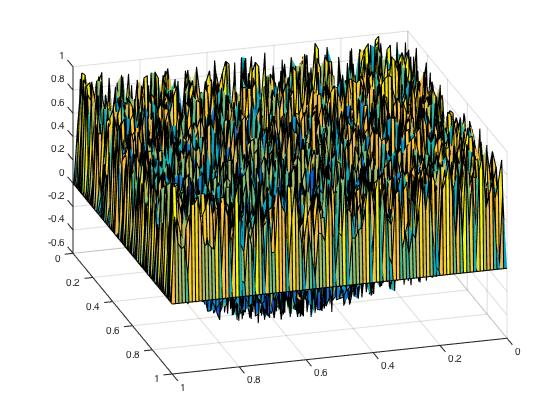
\includegraphics[width=5.5cm,height=5cm]{pictures/smooth0.jpg} \quad
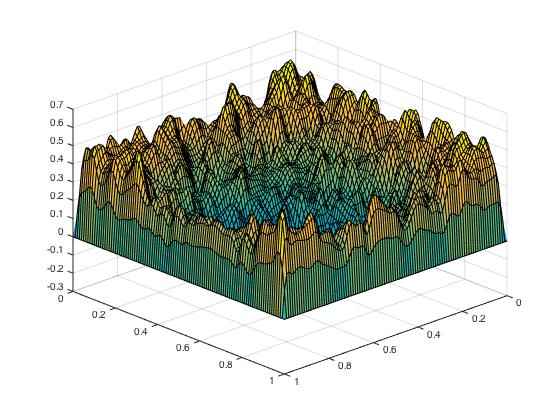
\includegraphics[width=5.5 cm,height=5cm]{pictures/smooth10.jpg}\quad
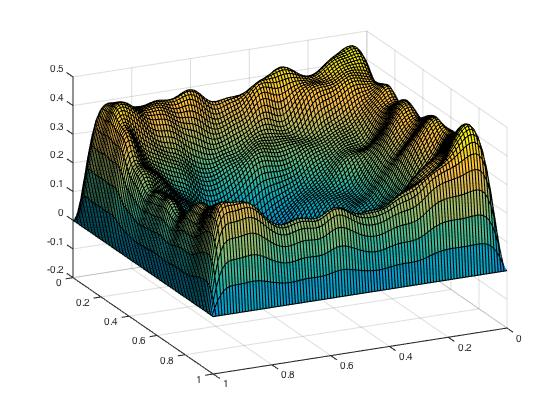
\includegraphics[width=5.5cm,height=5cm]{pictures/smooth50.jpg}\quad
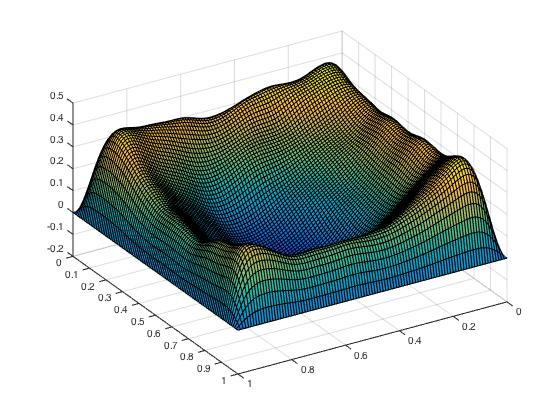
\includegraphics[width=5.5cm,height=5cm]{pictures/smooth100.jpg}
\caption{\footnotesize{The errors of an random initial guess $u^0$, $u^{10}$, $u^{50}$ and  $u^{100}$.}}
\label{fig:smooth}
\end{figure}
%\begin{figure}
%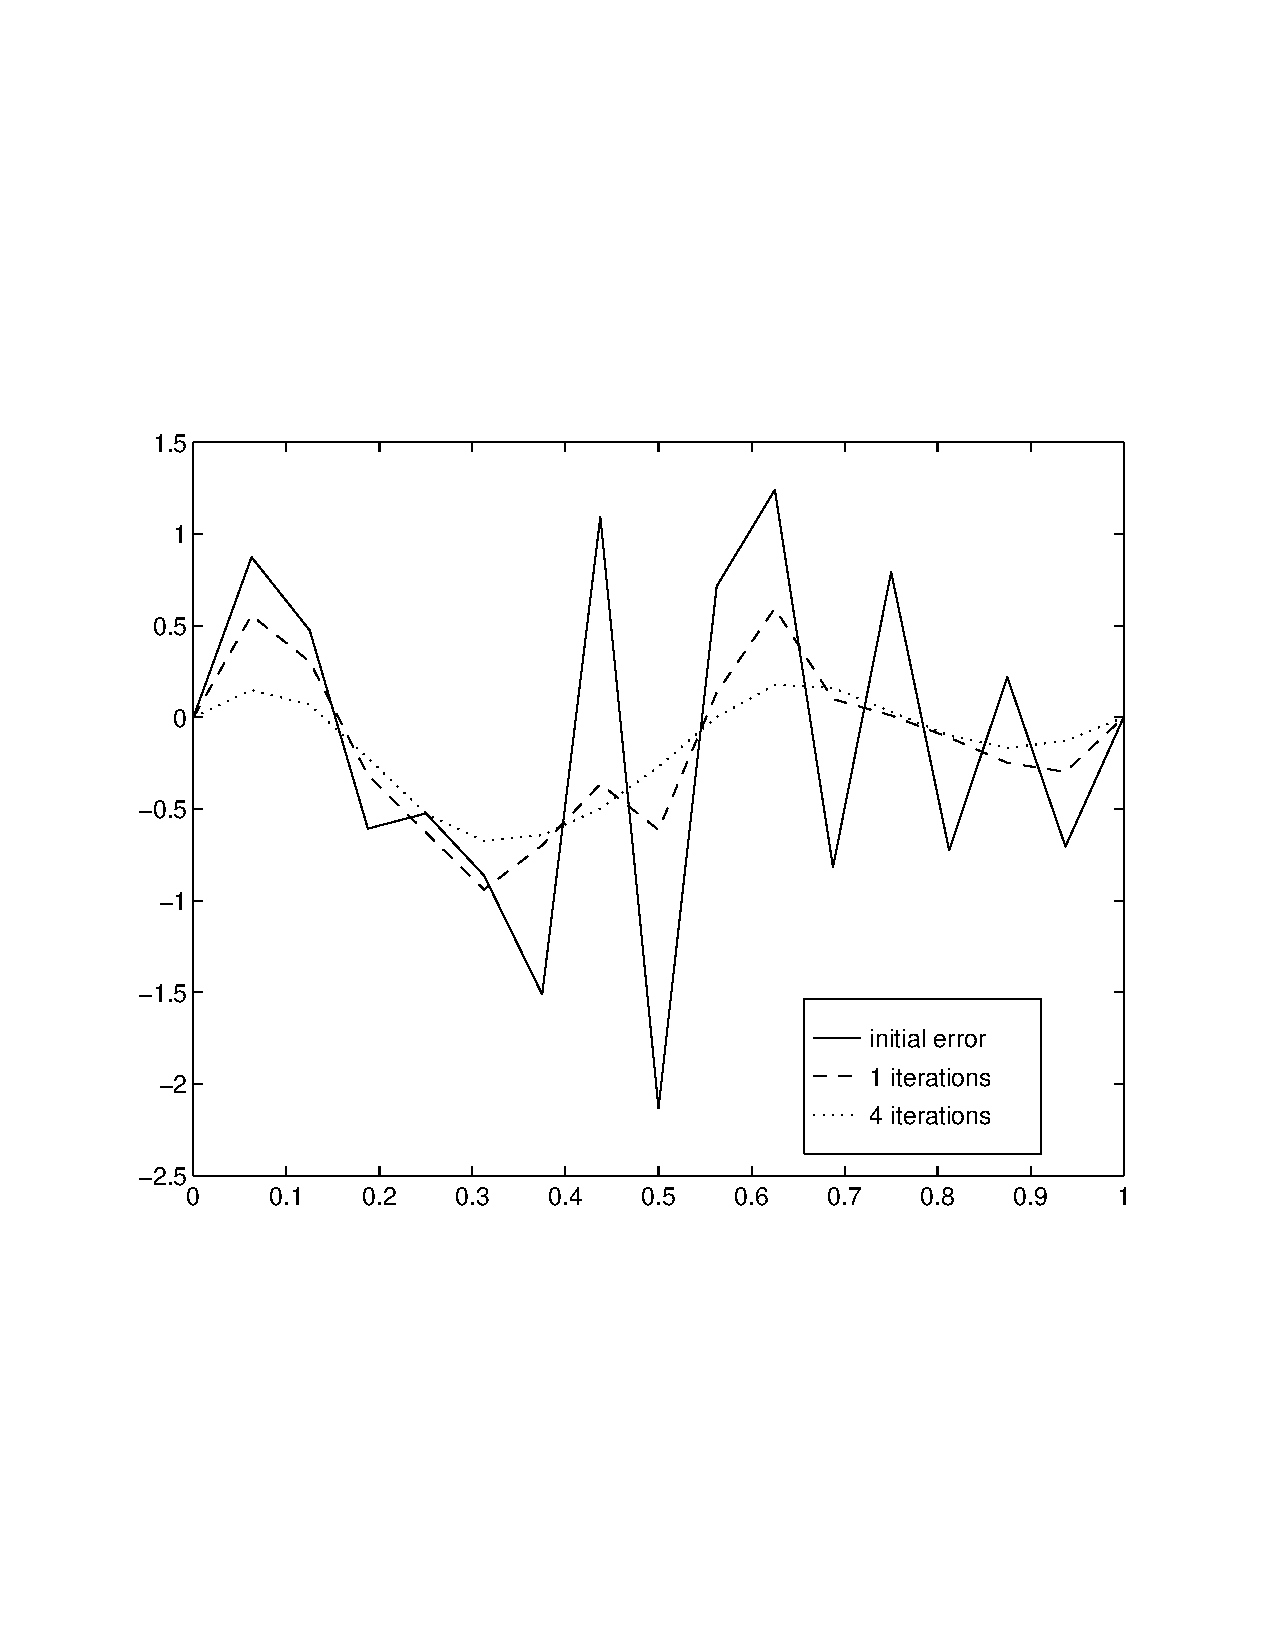
\includegraphics[width=12cm,height=8cm]{pictures/smoothing.pdf}
%\end{figure}
Next, we make the following particular choice:
\begin{equation}
  \label{eta}
\eta={1\over 8}.  
\end{equation}

The gradient descent method can be written in terms of $S_{0}:\mathbb
R^{m\times n}\mapsto \mathbb R^{m\times n}$ satisfying
\begin{equation}
\label{jacobi1}
u^1=(S_{0}f)={1\over 8} f,
\end{equation}
for equation \eqref{2d-fe0} with initial guess zero.
If we apply this method twice, then
$$
u^2=S_1(f) = S_{0} f + S_0(f - A\ast(S_{0}f)),
$$
with element-wise form
\begin{equation} 
\begin{aligned}
u^2_{i,j} &={3\over 16}f_{i,j} + {1\over 64}(f_{i+1,j}+f_{i-1,j}+f_{i,j+1}+f_{i,j-1}).
\end{aligned}
\end{equation}
Then by the definition of convolution \eqref{con1}, we have
 \begin{equation}\label{eq:convS}
u^1= S_{0}\ast f \quad u^2 = S_1 \ast f.
\end{equation}
with
\begin{equation}\label{eq:kernel-S}
S_{0} = {1 \over 8},
\end{equation}
and 
\begin{equation}\label{eq:kernel-S2}
S_1={1\over 64} \begin{pmatrix}
0 & 1 & 0 \\
1 & 12 & 1  \\
0 &1  & 0
\end{pmatrix}.
\end{equation}

Next, we make the following particular choice for the bilinear case:
\begin{equation}
  \label{eta}
\eta={1\over 16}.  
\end{equation}

The gradient descent method can be written in terms of $S_{0}:\mathbb
R^{m\times n}\mapsto \mathbb R^{m\times n}$ satisfying
\begin{equation}
\label{jacobi1}
u^1=(S_{0}f)_{i,j}={1\over 16} f_{i,j},
\end{equation}
for equation \eqref{2d-fe1} with initial guess zero.
If we apply this method twice, then
$$
u^2=S_1(f) = S_{0} f + S_0(f - A\ast(S_{0}f)),
$$
with element-wise form
\begin{equation} 
\begin{aligned}
u^2_{i,j} &={3\over 32}f_{i,j} + {1\over 256}(f_{i+1,j}+f_{i-1,j}+f_{i,j+1}+f_{i,j-1}+f_{i+1,j+1}+f_{i-1,j-1}+f_{i-1,j+1}+f_{i+1,j-1}).
\end{aligned}
\end{equation}
Then by the definition of convolution \eqref{con1}, we have
 \begin{equation}\label{eq:convS}
u^1= S_{0}\ast f \quad u^2 = S_1 \ast f.
\end{equation}
with
\begin{equation}\label{eq:kernel-S}
S_{0} = {1 \over 16},
\end{equation}
and 
\begin{equation}\label{eq:kernel-S2}
S_1={1\over 256} \begin{pmatrix}
1 & 1 & 1 \\
1 & 24 & 1  \\
1 &1  & 1
\end{pmatrix}.
\end{equation}




We note the gradient descent method \eqref{iterativeAst} can be written as
\begin{equation}\label{GD0}
u^k=u^{k-1} + S_0\ast (f-A\ast u^{k-1}).
\end{equation}
\begin{equation}\label{GD1}
u^{2k}=u^{2(k-1)} + S_1\ast (f-A\ast u^{2(k-1)}).
\end{equation}
We can sometimes use $S_1$ and the above identity to define a smoother
directly, namely 
\begin{equation}\label{GD2}
u^{k}=u^{k-1} + S_1\ast (f-A\ast u^{k-1}).
\end{equation}


Similarly, with the smoother obtained by \eqref{eq:convS}, we can define 
$S^{\ell}: \mathbb{R}^{m_\ell \times n_\ell} \mapsto \mathbb{R}^{m_\ell \times n_\ell}$.


First solve the problem on the fine grid $\mathcal T_{\ell}$, denote the solution by $u^{\ell}$, 
\begin{equation}\label{eq:smoothing0}
u^{\ell} \leftarrow u^{\ell} + S^\ell \ast (f^\ell - A_\ell \ast u^{\ell}).
\end{equation}
Denote the error by $e^\ell=u-u^{\ell}$ and the residual
\begin{equation}\label{eq:formresidual}
r^{\ell}=f-A_{\ell}\ast u^{\ell}.
\end{equation}
It is obvious that $A_{\ell}\ast e^\ell=r^{\ell}.$
We need to solve the residual equation
\begin{equation}\label{erreq}
A_{\ell}\ast e^\ell=r^{\ell}.
\end{equation}
The idea of multigrid method is to solve this residual equation on the coarse grid space $\mathcal V_{\ell+1}$ 
and repeat the process until coarsest grid. 

We note that the restriction of \eqref{erreq} to the coarse level $\ell+1$ is
\begin{equation}\label{coarse:correc}
A_{\ell+1}\ast e^{\ell+1}=r^{\ell+1}
\end{equation}
with $r^{\ell+1}=R_\ell^{\ell+1}r^\ell=R\ast r^\ell$.

Denote the finite element approximation to $e_\ell$ on the coarse grid $\mathcal T_{\ell+1}$ by $e_{\ell+1}$. Interpolate the error $e_{\ell+1}$ back to the fine space $\mathcal V_{\ell}$ and add the resulting residual to $u_{\ell+1}$, that is 
\begin{equation}\label{eq:prolongation00}
u^\ell \leftarrow u^{\ell}+P^{\ell}_{\ell+1}e^{\ell+1}
\end{equation}
%as defined in \eqref{mg-prolong} and restriction $R_{\ell}^{\ell+1} = (P_{\ell+1}^{\ell})^T$. 


Now using the smoother $S^\ell$, prolongation $P^{\ell}_{\ell+1}$, restriction $R_{\ell}^{\ell+1}$ and mapping
$A^\ell$ as given in \eqref{eq:def_coarse}, we can formulate the following algorithm
 as a major component of a multigrid algorithm.
\begin{breakablealgorithm}%[!htb]
	\caption{$(u^{1}, u^2, \cdots, u^J) = {\text{MG0}}(f; u^0; J,\nu_1, \cdots, \nu_J)$}
	\label{alg:L-Slash0}
	\begin{algorithmic}
		\State Set up
		$$
		f^1 = f, \quad u^{1}=u^0.
		$$
		\State Smoothing and restriction from fine to coarse level (nested)
		\For{$\ell = 1:J$}
		\For{$i = 1:\nu_\ell$}
		\State
		\begin{equation}\label{eq:smoothing}
		u^{\ell} \leftarrow u^{\ell} + S^\ell \ast (f^\ell - A_\ell \ast u^{\ell}).
		\end{equation}
		\EndFor
		\State Form restricted residual and set initial guess:
		$$
		u^{\ell+1,0} \leftarrow 0, \quad f^{\ell+1} \leftarrow R \ast_2 (f^\ell -  A_\ell \ast u^{\ell}), A_{\ell+1} = R \ast_2 A_\ell \ast (R\ast_2^\top).
		$$
		\EndFor
	\end{algorithmic}
\end{breakablealgorithm}
Here $S^\ell$ can be chosen as $S_0$ or $S_1$ as definition in \eqref{eq:kernel-S} and \eqref{eq:kernel-S2}.

Using the above algorithm, there are different multigrid algorithms such as: $\backslash$-cycle, V-cycle and W-cycle.
Let us now only give one special form of multigrid algorithm for solving \eqref{laplace} as follows.
\begin{breakablealgorithm}%[!htb]
	\caption{$u = {\text{MG1}}(f; u^0; J,\nu_1, \cdots, \nu_J)$}
	\label{alg:L-Slash1}
	\begin{algorithmic}
		\State 
		$$
		u \leftarrow u^0.
		$$
		\State
		$$
		(u^{1}, u^2, \cdots, u^J) = {\text{MG0}}(f; u; J,\nu_1, \cdots, \nu_J).
		$$
		\State Prolongation and restriction from coarse to fine level
		\For{$\ell = J-1:1$}
		\State
		$$
		u^{\ell} \leftarrow u^{\ell} + R  \ast_2^{\top} u^{\ell+1}.
		$$
%		%		\IF{V-cycle}
%		\For{$i = 1:\nu_\ell$}
%		\State
%		$$
%		u^{\ell,i} \leftarrow u^{\ell,i-1} + [B^{\ell,i}]^T (f^\ell - A^{\ell} u^{\ell,i-1})
%		$$
%		\EndFor
%		%		\ENDIF
		\EndFor
		\State
		$$
		u \leftarrow u^{1}.
		$$
	\end{algorithmic}
\end{breakablealgorithm}

If we add the post-smoothing with a symmetric form which means we 
use $[S^\ell \ast ]^\top$ as the smoother, then we can get the V-cycle
version multigrid algorithm.

\begin{breakablealgorithm}%[!htb]
	\caption{$u = {\text{MG2}}(f; u^0; J,\nu_1, \cdots, \nu_J; \nu'_1, \cdots, \nu'_J )$}
	\label{alg:V-cycle}
	\begin{algorithmic}
		\State 
		$$
		(u^{1}, u^2, \cdots, u^J) = {\text{MG0}}(f; u^0; J,\nu_1, \cdots, \nu_J).
		$$
		\State Prolongation and restriction from coarse to fine level
		\For{$\ell = J-1:1$}
		\State
		$$
		u^{\ell} \leftarrow u^{\ell} + R  \ast_2^{\top} u^{\ell+1}.
		$$
		\For{$i = 1:\nu'_\ell$}
		\State
		$$
		u^{\ell} \leftarrow u^{\ell} + S^\ell \ast (f^\ell - A_\ell \ast u^{\ell})
		$$
		\EndFor
				%		\ENDIF
		\EndFor
		\State 
		$$
		u = u^{1}.
		$$
	\end{algorithmic}
\end{breakablealgorithm}
Here $S^\ell $ means the central symmetry of kernel for smoother $S^\ell$ as in the 
definition of \eqref{eq:def_tildeK} in Lemma \ref{lemm:tilde-K}. 

We note that 
$$
\text{MG1}(f; u^0; J,\nu_1, \cdots, \nu_J) = {\text{MG2}}(f; u^0; J,\nu_1, \cdots, \nu_J; 0, \cdots, 0).
$$

Either MG1 or MG2 only represents one cycle in a multigrid process. There many  different ways
to use this basis multigrid cycle. For a given iterate $u$, we need to define a metric to measure the
accuracy of $u$. One way to define it is:
$$
\text{error}(u) = \|f - A\ast u\|  \big/ \|f - A\ast u^0\|.
$$
Sometimes, when we debug a code, we can first try to find the exact solution. $u_{\text{exact}}$, and
then define 
$$
\text{error}(u) = \| u_{\text{exact}} - u\|_A.
$$
Below is one example fo algorithm for application of the basic multigrid cycle, say MG1:
\begin{breakablealgorithm}%[!htb]
	\caption{$u = {\text{multigrid1}}(f; u^0; J,\nu_1, \cdots, \nu_J;  \text{tol})$;}
	\label{alg:multigrid-1}
	\begin{algorithmic}
		\State 
		$$
		u \leftarrow u^0.
		$$
		\While{$\text{error}(u) \ge tol $}
		\State
		$$
		u \leftarrow u + \text{MG1}(f-Au;0;\nu_1, \cdots, \nu_J).
		$$
		\EndWhile
	\end{algorithmic}
\end{breakablealgorithm}

A slightly more general multigrid method. 

\begin{breakablealgorithm}\label{alg:multigrid-Pi}
\begin{enumerate}
\item Initialization of inputs
		$$
		g_1 \leftarrow g, \quad
                u_{1}\leftarrow {\rm random}.
		$$
	\vspace{-.6mm}
\item Smoothing and restriction
  \begin{itemize}
  \item  For $\ell = 1:J$
    \begin{itemize}%3
    \item For $i = 1:\nu_\ell$
		\begin{equation}\label{eq:smoothing}
		u_{\ell} \leftarrow u_{\ell} + S_\ell \ast (g_\ell - A_\ell \ast u_{\ell}).
		\end{equation}
\item  Form restricted residual and set initial guess:
\begin{equation*}
u_{\ell+1,0} \leftarrow\Pi_\ell^{\ell+1}u_{\ell},  \quad g_{\ell+1} \leftarrow R_\ell \ast_2 (g_\ell -  A_\ell \ast u_{\ell}) + A_{\ell+1} \ast u_{\ell+1}^0,
\end{equation*}
    \end{itemize} %3
  \end{itemize}
\item  Prolongation with post-smoothing
  \begin{itemize} %4
  \item For {$\ell = J-1:1$}
		$$
		u_{\ell} \leftarrow u_{\ell} + R_\ell  \ast_2^{\top} (u_{\ell+1}-u_{\ell+1}^0).
		$$
		
                \begin{itemize}
  \item For $i = 1:\nu'_\ell$
		$$
		u_{\ell} \leftarrow u_{\ell} + S_\ell' \ast (g_\ell - A_\ell \ast u_{\ell})
		$$
                \end{itemize}
                \end{itemize} %4
\item Output
		$$
u_1
		$$
\end{enumerate} %1
\end{breakablealgorithm}

\section{Numerical examples}
We consider to solve 
\begin{equation}
\label{laplacenu}
-\Delta u = f,  \mbox{ in } \Omega,\quad
u=0  \mbox{ on } \partial\Omega,\quad
\Omega=(0,1)^2.
\end{equation}
For the $x$ direction and the $y$ direction, we consider the partition:
\begin{equation}\label{partitionyx}
 0=x_0<x_1<\cdots<x_{n+1}=1, \quad x_i=\frac{i}{n+1},\quad (i=0,\cdots,n+1);
 \end{equation}
 \begin{equation}\label{partitiony}
 0=y_0<y_1<\cdots<y_{n+1}=1, \quad y_j=\frac{j}{n+1},\quad (j=0,\cdots,n+1).
\end{equation}
We use linear finite to discretize the 2D Laplacian equation \eqref{laplacenu}.  The size of 
unknowns is $n^2$. We use gradient descent method as smoother in the multigrid method. 
\begin{table}\label{table:multivsGS}%[htdp]
\begin{center}
\begin{tabular}{|c||c|c|}
\hline \hline
Size of Unkowns & Gauss-Seidel for $A$ & Multigrid for $A$ \\ \hline\hline %& V + PCG for $A$\\ \hline %\hline
225  &  226/0.04s     &    13/0.004s \\ \hline %&\onslide<3->{\brown{5/0.003s}}  \\ \hline
961   &  910/0.26s      & 13/0.007s
\\ \hline %& \onslide<5->{\brown{5/0.005s}} \\ \hline 
3969   &  3,044/2.40s   &13/0.021s  \\ \hline %&  \onslide<7->{\brown{5/0.016s}} \\ \hline 
16,129   & 9,869/31.45s    &13/0.08s \\ \hline %& \onslide<9->{\brown{5/0.06s}}  \\ \hline 
65,025   &  30,226/347.38s  &13/0.3s\\ \hline %& \onslide<11->{\brown{5/0.22s}} \\   \hline \hline
\end{tabular}
\caption{Number of iterations for $\| Ax - b \|/ \|b\| \leq 10^{-6}$.}
\end{center}
\end{table}
\vspace{-30pt}
\begin{figure}[!ht]
\centering
%\setlength{\abovecaptionskip}{0pt}
%\setlength{\belowcaptionskip}{0pt}
\includegraphics[width=10cm]{figures/mgcompare.png}
\caption{ Comparison GD with Multigrid.}
\label{fig:Hmesh}
\end{figure}

From the Table \ref{table:multivsGS} and Figure \ref{fig:Hmesh}, we can see that the multigrid method is much faster than Gauss-Seidel method and is uniform with respect to the size of unknowns. 







\section{ReLU multigrid method for nonnegative solution}
Considering $f = (1, 1, ..., 1)^\top$,
\begin{breakablealgorithm}%[!htb]
	\caption{$(u^{1}, u^2, \cdots, u^J) = {\text{MG0}}(f; u^0; J,\nu_1, \cdots, \nu_J)$}
	\label{alg:L-ReLUSlash0}
	\begin{algorithmic}
		\State Set up
		$$
		f^1 = f, \quad u^{1}=u^0.
		$$
		\State Smoothing and restriction from fine to coarse level (nested)
		\For{$\ell = 1:J$}
		\For{$i = 1:\nu_\ell$}
		\State
		\begin{equation}\label{eq:smoothing}
		u^{\ell} \leftarrow u^{\ell} + S^\ell \ast \text{Relu}( (f^\ell - A_\ell \ast u^{\ell})).
		\end{equation}
		\EndFor
		\State Form restricted residual and set initial guess:
		$$
		u^{\ell+1,0} \leftarrow 0, \quad f^{\ell+1} \leftarrow R \ast_2 (f^\ell -  A_\ell \ast u^{\ell}), A_{\ell+1} = R \ast_2 A_\ell \ast (R\ast_2^\top).
		$$
		\EndFor
	\end{algorithmic}
\end{breakablealgorithm}
Algorithm 5 is not convergent.

\newpage
\begin{breakablealgorithm}%[!htb]
	\caption{$(u^{1}, u^2, \cdots, u^J) = {\text{MG0}}(f; u^0; J,\nu_1, \cdots, \nu_J)$}
	\label{alg:L-ReLUSlash1}
	\begin{algorithmic}
		\State Set up
		$$
		f^1 = f, \quad u^{1}=u^0.
		$$
		\State Smoothing and restriction from fine to coarse level (nested)
		\For{$\ell = 1:J$}
		\For{$i = 1:\nu_\ell$}
		\State
		\begin{equation}\label{eq:smoothing}
		u^{\ell} \leftarrow u^{\ell} +\text{Relu}( S^\ell \ast  (f^\ell - A_\ell \ast u^{\ell})).
		\end{equation}
		\EndFor
		\State Form restricted residual and set initial guess:
		$$
		u^{\ell+1,0} \leftarrow 0, \quad f^{\ell+1} \leftarrow R \ast_2 (f^\ell -  A_\ell \ast u^{\ell}), A_{\ell+1} = R \ast_2 A_\ell \ast (R\ast_2^\top).
		$$
		\EndFor
	\end{algorithmic}
\end{breakablealgorithm}

Algorithm 6 is convergent, the iterative steps is list below. $l = 2$
\\
\begin{tabular}{c|c|c|}
	J &MG& Algorithm 6\\ \hline
	2 & 15 & 27 \\\hline
	3 & 16 & 35 \\\hline
	4 & 17 & 38 \\\hline
\end{tabular}


\subsection{$\Pi$ is interpolation}
\textbf{Not Convergent}
		\begin{equation}
		u^{\ell,i} \leftarrow u^{\ell,i-1} + \text{Relu}\circ B_{\ell,i}  ({f^\ell -  A^{\ell} (u^{\ell,i-1})}).
		\end{equation}
	 \begin{equation}
	 u^{\ell,i} \leftarrow u^{\ell,i-1} + B_{\ell,i}\circ\text{Relu}({f^\ell -  A^{\ell} (u^{\ell,i-1})}).
	 \end{equation}
\textbf{Almost the same as without Relu}
	 \begin{equation}
	 u^{\ell,i} \leftarrow u^{\ell,i-1} +B_{\ell,i}  ({f^\ell -   \text{Relu}\circ A^{\ell} (u^{\ell,i-1})}).
	 \end{equation}
	 \begin{equation}
	 u^{\ell,i} \leftarrow u^{\ell,i-1} + B_{\ell,i}  ({f^\ell -  A^{\ell} \circ\text{Relu}(u^{\ell,i-1})}).
	 \end{equation}
\section{Multigrid methods for nonlinear problem}
In classification, the key problem can be reduced to find the 
representation (feature) for high dimension image for classifying. 
Here we propose to solve the next unbalanced nonlinear system  
\begin{equation}\label{eq:rep}
L(u) = f,
\end{equation}
for finding the suitable feature representation $u \in \mathbb{R}^c$ for  
image $f\in \mathbb{R}^{n}$. The rationality of system can be traced back to 
the low-dimension assumption that natural image need to be concentrated 
on a low-dimension manifold with respect to the pixel space.

In order to motivate how to deal with the nonlinear system \eqref{eq:rep}, we 
consider a simple nonlinear model problem 
\begin{equation}\label{nonlinear:poisson}
\left\{
\begin{aligned}
-\nabla\cdot(a(u)\nabla u)+c(u)&=f, \quad x\in \Omega,\\
u&=0\quad\hbox{on}\quad\partial \Omega.
\end{aligned}
\right. 
\end{equation}
%\example $p$-Laplacian $\displaystyle \min_{u\in W^{1,p}()\Omega} \frac{1}{p} \int_\Omega |\nabla u|^p dx-\int_\Omega fudx$. 

The weak formulation of \eqref{nonlinear:poisson} reads: Find $u\in H^1_0(\Omega)$, such that 
$$
(a(u)\nabla u,\nabla v)+(c(u), v)=(f,v), \quad \forall v\in H^1_0(\Omega). 
$$
Define
\begin{equation}
(L(u), v)=(a(u)\nabla u,\nabla v)+(c(u), v).
\end{equation}
Then we have 
\begin{equation}
L(u)=f.
\end{equation}
Now the discretization problem reads: Find $u_h\in V_h$ such that
\begin{equation}
(a(u_h)\nabla u_h,\nabla v_h)+(c(u_h), v_h)=(f,v_h)\quad \forall v_h\in V_h. 
\end{equation}
Again define 
$$
(L_h(u_h), v_h)=(a(u_h)\nabla u_h,\nabla v_h)+(c(u_h), v_h).
$$
Then we obtain 
\begin{equation}\label{non:system}
L_h(u_h)=f_h. 
\end{equation}
If $a(u_h)$ is a constant, then \eqref{non:system} reduces to a linear system and we denote the 
linear system as $A_hu_h=f_h$. 

Recall the two grid method described in \eqref{eq:smoothing0}, \eqref{eq:formresidual}, \eqref{erreq}, \eqref{coarse:correc} and \eqref{eq:prolongation00}
for linear problem 
\begin{equation}\label{linearA}
A_hu_h=f_h,
\end{equation}
reads as following three steps:
\begin{enumerate}
\item Fine grid smoothing: 
%applying $m$ times gradient descent iterations to obtain $u^m$.
$$
u_h\update u_h+S_h(f_h-A_hu_h)
$$
such as gradient descent method. 
\item Coarse grid correction: solving the residual equation restricted
on the coarse grid $\ct_{2h}$ to obtain
$$
        A_{2h}e_{2h}=Q_{2h}r^h
$$
with $r^h=f_h-A_h u_h$. 
\item Update: $u_h\update u_h+e_{2h}$.
\end{enumerate}
Coarse grid correction for the linear case can be rewritten as: 
$$
 A_{2h}e_{2h}=Q_{2h}(f_h-A_h u_h).
 $$
 For any $u_h^0$, we write the above equation as  
 \begin{equation}\label{eq2}
Q_{2h}(A_{h}(u_h^0+e_{2h})-A_hu_h^0)=Q_{2h}(f_h-A_h u_h).
 \end{equation}
 Noting that $Q_{2h}A_{h}=A_{2h}P_{2h}$, where $P_{2h}$ is the energy projection 
%from $V_h$ 
 into $V_{2h}$. 
 Therefore \eqref{eq2} can be written as 
% $$
% A_{2h}(P_{2h} u_h^0)+ A_{2h} e_{2h})- A_{2h} (P_{2h} u_h^0)=Q_{2h}(f_h-A_h u_h).
% $$
% and further 
  \begin{equation}\label{eq4}
 A_{2h}(P_{2h} u_h^0+ e_{2h})=Q_{2h}(f_h-A_h u_h)+A_{2h} (P_{2h} u_h^0).
  \end{equation}
Now let 
$$
u_{2h,0}=P_{2h} u_h^0 \quad \hbox{and}\quad u_{2h}=P_{2h} u_h^0+ e_{2h},
$$
 then solving $e_{2h}$ in  \eqref{eq4} is equivalent to solve $u_{2h}$  in the following equation
\begin{equation}\label{eq5}
 A_{2h}u_{2h}=Q_{2h}(f_h-A_h u_h)+A_{2h} (u_{2h,0}).
 \end{equation}
 In this case, noting that $e_{2h}=u_{2h}-P_{2h} u_h^0=u_{2h}-u_{2h,0}$, hence the step 3 means 
 $$
\hbox{ Update:} \,\, u_h\update u_h+u_{2h}-u_{2h,0}.
 $$
 
 In summery, the two grid method for the linear system \eqref{linearA} can be rewritten as following three steps:
\begin{enumerate}
\item Fine grid smoothing: 
%applying $m$ times gradient descent iterations to obtain $u^m$.
$$
u_h\update u_h+S_h(f_h-A_hu_h)
$$
such as gradient descent method. 
\item Coarse grid correction: for any $u_h^0$, solving the residual equation restricted
on the coarse grid $\ct_{2h}$ to obtain
$$
   u_{2h,0}=P_{2h} u_h^0, \quad     A_{2h}u_{2h}=Q_{2h}(f_h-A_h u_h)+A_{2h} (u_{2h,0}).
$$
where $P_{2h}$ is the energy projection %from $V_h$ 
into $V_{2h}$. 
\item Update: $u_h\update u_h+u_{2h}-u_{2h,0}$.
\end{enumerate}
Usually, after the fine grid smoothing, we choose $u_h^0$ as the solution updated from the fine grid smoothing.  And for nonlinear problems, we replace $P_{2h}u_h^0$ by $\Pi_h^{2h}u_h^0$, where $\Pi_h^{2h}$ is an interpolation or projection from $V_h$ to $V_{2h}$. 
Now we apply the above two grid method to the nonlinear system \eqref{non:system}, 
namely $L_{h}(u_h)=f_h$, we obtain the two grid method for nonlinear system
 \begin{enumerate}
\item Fine grid smoothing: 
%applying $m$ times gradient descent iterations to obtain $u^m$.
$$
u_h\update u_h+S_h(f_h-L_h(u_h))
$$
such as gradient descent method. 
\item Coarse grid correction: solving the residual equation restricted
on the coarse grid $\ct_{2h}$ to obtain
$$
   u_{2h,0}=\Pi_h^{2h} u_h, \quad     L_{2h}(u_{2h})=Q_{2h}(f_h-L_h (u_h))+L_{2h} (u_{2h,0}).
$$
where $\Pi_h^{2h}$ is an interpolation or projection from $V_h$ to $V_{2h}$. 
\item Update: $u_h\update u_h+u_{2h}-u_{2h,0}$. 
\end{enumerate}

 
To solve the nonlinear system, we can try the multilevel ideas 
with smoothing in fine level, and truncated it into coarse level by recursion. 
One strategy to involve the multi-scale idea is to ``smoothing'' in the fine level, 
and restrict it as a good approximation in the coarse level, this idea can 
be found in many literatures especially for multigrid methods in optimization 
\cite{tai2002global, nash2000a}.  So, there is a more general nonlinear multigrid named 
scheme-fully approximation scheme (FAS) \cite{briggs2000a, trottenberg2000multigrid}, 
which can be considered as the generalization of linear multigrid Algorithm \ref{alg:L-Slash1}.  
Here we show a FAS algorithm with V-cycle as
\begin{breakablealgorithm}
	\caption{$u = {\text{ Bslash-FAS}}(u^{1,0},f,J,m_1, \cdots, m_J)$}
	\label{alg:Slash-FAS}
	\begin{algorithmic}
		\State Initialization 
		$$
		f^1 = f.
		$$
		\State Smoothing and restriction from fine to coarse level (nested)
		\For{$\ell = 1:J$}
		\State Nonlinear relaxation on level $\ell$:
		\For{$i = 1:m_j$}
		\State 
		$$
		u^{\ell,i} = u^{\ell,i-1} +S_\ell^i(f^\ell - L^{\ell}(u^{\ell,i-1})).
		$$
		\EndFor
		\State Form the initial guess and right side term for level $\ell+1$:
		$$
		u^{\ell+1,0} = \Pi_\ell^{\ell+1}u^{\ell,m_\ell}, \quad 
		f^{\ell+1} = R_\ell^{\ell+1} (f^\ell - L^{\ell}(u^{\ell,m_\ell})) + L^{\ell+1}( u^{\ell+1, 0}).
		$$
		\EndFor
		\State Prolongation and correction from coarse to fine level
		\For{$\ell = J-1:1$}
		
		\State Form error in coarse level 
		$$
		e^{\ell+1} = u^{\ell+1, m_{\ell+1}} - u^{\ell+1,0}.
		$$
		\State Correction by using error in coarse level
		$$
		u^{\ell,m_\ell} \leftarrow u^{\ell,m_\ell} + P_{\ell+1}^{\ell}e^{\ell+1}.
		$$
		\EndFor
	\end{algorithmic}
\end{breakablealgorithm}
%For some cases, we choose $S_\ell^i=[\nabla F^{\ell}(u^{\ell,i-1})]^{-1}$.
If the problem in \eqref{eq:rep} is linear, then we have the next theorem to show that 
this FAS scheme is consist with the classical multigrid methods for linear systems.
\begin{theorem}
	If $L(u)$  in \eqref{eq:rep}  is a linear operation. 
	Then Algorithm \ref{alg:Slash-FAS} is equivalent to Algorithm \ref{alg:L-Slash1} with any choice of $\Pi_\ell^{\ell+1}$.
\end{theorem}


\section{A nonlinear BVP example}
 Consider the following boundary value problem
$$
-u''+2u^3=0 \quad(0< x < 1), \quad u(0)=\frac{1}{3}\hbox{~and~}u(1)=\frac{1}{4}.
$$
The analytical solution is  $u=\frac{1}{x+3}$. The weak formulation becomes
\begin{equation}
(u',v')+(2u^3,v)=0.
\end{equation}
By choosing $u_h=\sum \alpha_i \phi_i$, we have
\begin{equation}\label{eq:nolinear}
L_h({\bm \alpha}):=A{\bm \alpha}+2h{\bm \alpha}^3-b,
\end{equation}
where
$A =\frac{1}{h}
\begin{pmatrix}
2 & -1 &  &&\\
-1 & 2 & -1&&\\
   &\vdots&\vdots&\vdots&\\
   &&-1&2&-1\\
   &&&-1&2
\end{pmatrix}$ and
$b =\frac{1}{h}
\begin{pmatrix}
\frac{1}{3}\\
\vdots\\
\frac{1}{4}\end{pmatrix}$.  
We use gradient descent method and nonlinear multigrid method to solve \eqref{eq:nolinear}. The smoother used in the 
nonlinear multigrid method is two steps of gradient descent method: 
$$
\bm \alpha^{n+1}=\bm \alpha^n-\eta L_h(\bm \alpha^n) -\eta L_h(\bm \alpha^n-\eta L_h(\bm \alpha^n))
$$
where $L_h$ is defined by \eqref{eq:nolinear} and $\eta$ is the learning rate. 

\begin{table}\label{Table:nonliear}%[htdp]
\begin{center}
\begin{tabular}{|c||c|c|}
\hline \hline
Size of Unkowns  & Nonlinear Multigrid  ethod  & Gradient Descent method \\ \hline\hline %& V + PCG for $A$\\ \hline %\hline
15       &   13 steps  &  61.6 k steps \\ \hline %&\onslide<3->{\brown{5/0.003s}}  \\ \hline
31      &   14 steps   &  976.6 k steps  \\ \hline %&\onslide<3->{\brown{5/0.003s}}  \\ \hline
63         &  15 steps & $>$ 1000 k steps\\ \hline %& \onslide<5->{\brown{5/0.005s}} \\ \hline 
127       & 16 steps & $>$ 1000 k steps \\ \hline %&  \onslide<7->{\brown{5/0.016s}} \\ \hline 
255        & 16 steps & $>$ 1000 k steps \\ \hline %& \onslide<9->{\brown{5/0.06s}}  \\ \hline 
511     &17 steps& $>$ 1000 k steps \\ \hline %& \onslide<11->{\brown{5/0.22s}} \\   \hline \hline
1023      &18 steps&$>$ 1000 k steps \\ \hline %& \onslide<11->{\brown{5/0.22s}} \\   \hline \hline
\end{tabular}
\caption{Number of iterations for $\| L_h({\bm \alpha}) \|/ \|b\| \leq 10^{-6}$}
\end{center}
\end{table}

From the above numerical results shown in Table \ref{Table:nonliear}, the nonlinear multigrid method is uniform with respect to the size of 
unknowns and much faster than the gradient descent method.  


\endinput
Following the FAS idea, we propose the next Algorithms \ref{alg:OD-FAS} to solve the \eqref{eq:rep}:
\begin{breakablealgorithm}
	\caption{$u = {\text{OD-FAS}}(f,J,m_1, \cdots, m_J)$}
	\label{alg:OD-FAS}
	\begin{algorithmic}
		\State Initialization
		$$
		u^{1,0} = f,
		$$
		\State Feature extraction between levels,
		\For{$\ell = 1:J$}
		\State Feature extraction during level $\ell$,
		\For{$i = 1:m_\ell$}
		\State 
		$$
		u^{\ell,i} = u^{\ell,i-1} +[\epsilon I + \nabla F^{\ell}(u^{\ell,i-1})]^{-1} (f^\ell - F^{\ell}(u^{\ell,i-1})).
		$$
		\EndFor
		\If{$\ell = J$}
		\State Return $u^{J,m_J}$.
		\EndIf
		\State Form initialization and right hand term in coarse level:
		$$
		u^{\ell+1,0}= R_\ell^{\ell+1} u^{\ell,m_\ell}, \quad 
		f^{\ell+1} = R_\ell^{\ell+1} (r^\ell - F^{\ell}(u^{\ell,m_\ell})) + F^{\ell+1}( u^{\ell+1, 0}).
		$$
		\EndFor
	\end{algorithmic}
\end{breakablealgorithm}



%%%%%%%%%%%%%%%%%%%%%%%%%%%%%%%%%%
